\thispagestyle{empty}
\addcontentsline{toc}{chapter}{EXAMEN GENERAL 2024-I}
\addcontentsline{toc}{section}{Primera Etapa}

\vspace*{\fill}
\begin{center}
	{\Huge\bfseries EXAMEN GENERAL 2024-I}\\[10pt]
	{\Large\bfseries Primera Etapa}
\end{center}
\vspace*{\fill}

\clearpage




\section*{Área: Ingenierías}


\subsection*{Aritmética}

\begin{enumerate}
	
	
	\item Si: 
	$A = \{ a \in \mathbb{Z} / a^5 - 5a^3 + 4a = 0 \}$ \\
	$B = \{ a \in A / \exists \, b \in \mathbb{Z}, a = b^2 \}$ \\
	Halle la suma de los elementos de $A - B$.
	
	\begin{enumerate}[label=\alph*)]
	\item 0
	\item 1
	\item -1
	\item -2
	\item 2
	\end{enumerate}
	
	\textbf{Respuesta correcta:} a)
	
	\vspace{2mm}
	\textbf{Solucionario:}\\[1mm]
	Con $A$: 
	\begin{align*}
		a^5 - 5a^3 + 4a = 0 &\Rightarrow a(a^4 - 5a^2 + 4) = 0 \\
		&\Rightarrow a(a^2 - 1)(a^2 - 4) = 0 \\
		&\Rightarrow a(a-1)(a+1)(a-2)(a+2) = 0
	\end{align*}
	Entonces: $A = \{ -2; -1; 0; 1; 2 \}$
	
	Con $B$: Para $a = -2 \vee a = -1$, no existe un $b \in \mathbb{Z} / a = b^2$. \\
	$a = 0 \Rightarrow \exists \, b \in \mathbb{Z} / 0 = b^2 \rightarrow b = 0$ \\
	$a = 1 \Rightarrow \exists \, b \in \mathbb{Z} / 1 = b^2 \rightarrow b = -1, 1$ \\
	$a = 2 \Rightarrow \nexists \, b \in \mathbb{Z} / 2 = b^2$
	
	Entonces: $B = \{ 0; 1; -1 \}$
	
	Luego: $A - B = \{ -2; 2 \}$
	
	Piden la suma de sus elementos de $A - B$: $-2 + 2 $\fbox{$= 0$}
	
	
	\vspace{6mm}
	

	\item Hallar el número de seis cifras cuya primera cifra a la izquierda es uno y tal que si esta cifra se traslada a la derecha de la cifra de las unidades, el número así formado es el triple del original.
	
	\begin{enumerate}[label=\alph*)]
		\item $181534$
		\item $121337$
		\item $112857$
		\item $142857$
		\item $135682$
	\end{enumerate}
	
	\textbf{Respuesta correcta:} d)
	
	\vspace{2mm}
	\textbf{Solucionario:}\\[1mm]
	Sea el número: $\overline{1abcde}$ \\
	Dato: $\overline{abcde1} = 3(\overline{1abcde})$
	
	Descomponiendo resulta:
	\begin{align*}
		10(\overline{abcde}) + 1 &= 3(10^5 + \overline{abcde}) \\
		10(\overline{abcde}) + 1 &= 300\,000 + 3(\overline{abcde}) \\
		7(\overline{abcde}) &= 300000 - 1 \\
		7(\overline{abcde}) &= 299999 \\
		\overline{abcde} &= 42857
	\end{align*}
	
	Piden $\overline{1abcde} $ \fbox{$= 142857$}
	
	\vspace{6mm}
	
	\item Si $N$ es un número que descompuesto en sus factores primos es igual a $N = 2^5 \cdot 3^4 \cdot x$ y además $N$ es igual a $\dfrac{24}{77}$ de la suma de sus divisores, halle  la suma de digitos de $x$.
	
	\begin{enumerate}[label=\alph*)]
		\item $3$
		\item $2$
		\item $8$
		\item $6$
		\item $10$
	\end{enumerate}
	
	\textbf{Respuesta correcta:} b)
	
	\vspace{2mm}
	\textbf{Solucionario:}\\[1mm]
	Usamos la fórmula para hallar $S.D_{(N)}$ (Suma de Divisores). \\
	Como $N = 2^5 \cdot 3^4 \cdot x^1$, entonces:
	
	$ N = \dfrac{24}{77} \cdot (S.D_{(N)}) $
	
	$N = \dfrac{24}{77} \left[ \left( \dfrac{2^6 - 1}{2 - 1} \right) \left( \dfrac{3^5 - 1}{3 - 1} \right) \left( \dfrac{x^2 - 1}{x - 1} \right) \right] $
	
		$2^5 \cdot 3^4 \cdot x = \dfrac{24}{77} \cdot \dfrac{63}{1} \cdot \dfrac{242}{2} \cdot (x + 1)$ \\
		
		$2^5 \cdot 3^4 \cdot x = 2^3 \cdot 3^3 \cdot 11 \cdot (x + 1)$ \\
		$2^2 \cdot 3 \cdot x = 11x + 11 $\\
		$12x = 11x + 11 \Rightarrow x = 11$

	
	Suma de cifras de $x$: $1 + 1 $\fbox{$= 2$}
	
	\vspace{6mm}
	
	
	
	\item Se tiene la siguiente distribución de frecuencias respecto al ingreso familiar de 200 familias.
	
	\begin{center}
		\begin{tabular}{|c|c|c|}
			\hline
			Ingreso & $f_i$ & $F_i$ \\ \hline
			$[ \quad ; \quad \rangle$ & 35 & \\ \hline
			$[ \quad ; 240 \rangle$ & & \\ \hline
			$[ \quad ; \quad \rangle$ & 45 & 120 \\ \hline
			$[ \quad ; \quad \rangle$ & & 157 \\ \hline
			$[ 280; \quad \rangle$ & & \\ \hline
			$[ \quad ; \quad ]$ & 20 & \\ \hline
		\end{tabular}
	\end{center}
	
	¿Cuántas familias tienen un ingreso entre S/. 230 y S/. 300?
	
	\begin{enumerate}[label=\alph*)]
		\item 125
		\item 120
		\item 68
		\item 124
		\item 86
	\end{enumerate}
	
	\textbf{Respuesta correcta:} a)
	
	\vspace{2mm}
	\textbf{Solucionario:}\\[1mm]
	Calculamos el ancho de clase ($w$):
	
	% Representación del gráfico de intervalos
	\begin{center}
		\setlength{\unitlength}{1mm}
		\begin{picture}(80,10)
			\put(0,5){\line(1,0){70}}
			\put(0,5){\circle*{1.5}} \put(14,5){\circle*{1.5}} \put(28,5){\circle*{1.5}} 
			\put(42,5){\circle*{1.5}} \put(56,5){\circle*{1.5}} \put(70,5){\circle*{1.5}}
			\put(6,7){\small $w=20$} \put(20,7){\small $w=20$} \put(34,7){\small $w=20$} \put(48,7){\small $w=20$} \put(62,7){\small $w=20$}
			\put(26,1){\small 240} \put(54,1){\small 280}
		\end{picture}
	\end{center}
	
	Se observa: $2w = 40 \Rightarrow w = 20$.
	
	Luego, distribuimos las frecuencias en los intervalos:
	\begin{itemize}
		\item $[200; 220\rangle \rightarrow f_1 = 35$
		\item $[220; 240\rangle \rightarrow f_2 = 120 - 35 - 45 = 40$
		\item $[240; 260\rangle \rightarrow f_3 = 45$
		\item $[260; 280\rangle \rightarrow f_4 = 157 - 120 = 37$
		\item $[280; 300\rangle \rightarrow f_5 = 200 - 157 - 20 = 23$
		\item $[300; 320] \rightarrow f_6 = 20$
	\end{itemize}
	
	Para el rango entre S/. 230 y S/. 300:
	\begin{itemize}
		\item Del intervalo $[220; 240\rangle$, tomamos la mitad (de 230 a 240): $40 / 2 = 20$ familias.
		\item Del intervalo $[240; 260\rangle$: 45 familias.
		\item Del intervalo $[260; 280\rangle$: 37 familias.
		\item Del intervalo $[280; 300\rangle$: 23 familias.
	\end{itemize}
	
	Suma total: $20 + 45 + 37 + 23 $\fbox{$ = 125$}.
	
	Por lo tanto, hay 125 familias que tienen ingresos entre S/. 230 y S/. 300.
	
	

	
	\vspace{6mm}

\end{enumerate}




\subsection*{Álgebra}


\begin{enumerate}[resume]
	
	
	\item Sabiendo que $f(x) = 6x + k$ y $g(x) = 4x - k$, halle el valor de $k$ si se cumple $(f \circ g)(x) + 4 = (g \circ f)(x) - (f - g)(k)$.
	
	\begin{enumerate}[label=\alph*)]
		\item 1
		\item -1
		\item 2
		\item -2
		\item 0
	\end{enumerate}
	
	\textbf{Respuesta correcta:} a)
	
	\vspace{2mm}
	\textbf{Solucionario:}\\[1mm]
	Calculamos las composiciones y la resta:
	\begin{itemize}
		\item $(f \circ g)(x) = f(4x - k) = 6(4x - k) + k = 24x - 5k$
		\item $(g \circ f)(x) = g(6x + k) = 4(6x + k) - k = 24x + 3k$
		\item $(f - g)(k) = f(k) - g(k) = (6k + k) - (4k - k) = 7k - 3k = 4k$
	\end{itemize}
	Reemplazamos en la ecuación original:
	\begin{align*}
		(24x - 5k) + 4 &= (24x + 3k) - 4k \\
		24x - 5k + 4 &= 24x - k \\
		-4k + 4 &= 0 \\
		4 &= 4k \Rightarrow \fbox{k = 1}
	\end{align*}
	
	
	
	
	
	\vspace{6mm}
	
	
	
	
	\item Sean $A$ y $B$ matrices cuadradas del mismo orden. Establezca el valor de verdad de las siguientes proposiciones:
	\begin{enumerate}[label=\Roman*.]
		\item $(A + B)^2 = A^2 + 2AB + B^2$
		\item $|A + B| = |B + A|$
		\item $|A \cdot B| = |A| |B|$
		\item $|A \cdot B^{-1}| =\displaystyle \dfrac{|A|}{|B|}, \text{ donde } |B| \neq 0$
	\end{enumerate}
	
	\begin{enumerate}[label=\alph*)]
		\item FVVV
		\item VFVV
		\item VVVF
		\item VVFF
		\item FFVF
	\end{enumerate}
	
	\textbf{Respuesta correcta:} a)
	
	\vspace{2mm}
	\textbf{Solucionario:}\\[1mm]
	\begin{itemize}
		\item \textbf{I. (F)} Pues $(A + B)^2 = A^2 + AB + BA + B^2$. 
		\item \textbf{II. (V)} La suma de matrices es conmutativa, 
		\item \textbf{III. (V)} Propiedad de los determinantes: el determinante del producto es el producto de los determinantes.
		\item \textbf{IV. (V)} Propiedad de los determinantes: $|B^{-1}| = \displaystyle\dfrac{1}{|B|}$.
	\end{itemize}
	
	
	
	\vspace{6mm}
	
	
	\item Al descomponer $\displaystyle\dfrac{x+1}{(x-1)^3}$ en una suma de fracciones parciales, se encontró que uno de sus sumandos es $\displaystyle\dfrac{A_2}{(x-1)^2}$. ¿Cuál es el valor de $A_2$?
	
	\begin{enumerate}[label=\alph*)]
		\item 1
		\item -1
		\item 2
		\item -2
		\item 3
	\end{enumerate}
	
	\textbf{Respuesta correcta:} a)
	
	\vspace{2mm}
	\textbf{Solucionario:}\\[1mm]
	Planteamos la descomposición:
	\[ \dfrac{x+1}{(x-1)^3} = \dfrac{A_1}{(x-1)} + \dfrac{A_2}{(x-1)^2} + \dfrac{A_3}{(x-1)^3} \]
	Multiplicando todo por $(x-1)^3$:
	\[ x + 1 = A_1(x-1)^2 + A_2(x-1) + A_3 \]
	\[ x + 1 = A_1(x^2 - 2x + 1) + A_2x - A_2 + A_3 \]
	
	Comparando coeficientes:
	\begin{itemize}
		\item Para $x^2$: $A_1 = 0$
		\item Para $x$: $A_2 - 2A_1 = 1 \Rightarrow A_2 - 0 = 1 \Rightarrow A_2 = 1$
		\item Término independiente: $A_1 - A_2 + A_3 = 1 \Rightarrow 0 - 1 + A_3 = 1 \Rightarrow A_3 = 2$
	\end{itemize}
	Por lo tanto, \fbox{$A_2 = 1$}.
	
	
	
	
	\item Halle el volumen máximo de un cilindro, cuya área total es igual a $S$.
	
	\begin{enumerate}[label=\alph*)]
		\item $\displaystyle\dfrac{\pi s^{\dfrac{3}{2}}}{2}$
		\item $\pi$
		\item $\displaystyle\dfrac{s^{\dfrac{3}{2}}}{3\sqrt{6\pi}}$
		\item $\displaystyle\dfrac{\pi}{2} S^3$
		\item $\pi S^{\dfrac{3}{2}}$
	\end{enumerate}
	
	\textbf{Respuesta correcta:} a)
	
	\vspace{2mm}
	\textbf{Solucionario:}\\[1mm]
	$V = \pi r^2 h$ y $S = 2\pi r^2 + 2\pi r h$ \\
	
	Despejamos $h$: $h = \dfrac{S - 2\pi r^2}{2\pi r}$ \\
	
	Luego reemplazamos en $V$:
	
	$V = \pi r^2 \left( \dfrac{S - 2\pi r^2}{2\pi r} \right) = \dfrac{r}{2}(S - 2\pi r^2) = \dfrac{rS}{2} - \pi r^3 $\\
	
	Derivamos para maximizar:\\
	$V' = \dfrac{S}{2} - 3\pi r^2 = 0 \Rightarrow r^2 = \dfrac{S}{6\pi} \Rightarrow r = \sqrt{\dfrac{S}{6\pi}}\\ $
	 $V'' = -6\pi r < 0$ (es un máximo). \\
	 $V = \dfrac{rS}{2} - \dfrac{rS}{6} = \dfrac{rS}{3}\\$ 
	\fbox{$V = \displaystyle\dfrac{s^{\dfrac{3}{2}}}{3\sqrt{6\pi}}$} \\
	
	
	\vspace{6mm}
	
\end{enumerate}


\subsection*{Geometría}

\begin{enumerate}[resume]
	
	\item En la figura, P=(6$\sqrt{3};8$). Halle la distancia del baricentro de la región triángular UNO al punto P.
	
	
	\begin{center}
		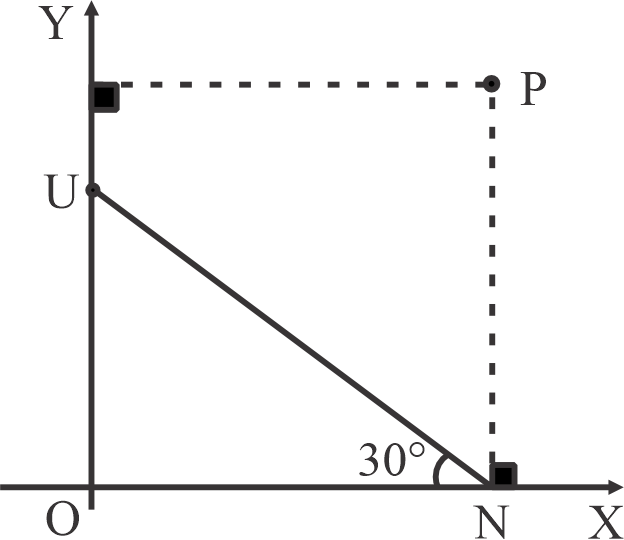
\includegraphics[width=3.5cm]{imagenes/general2024-I/etapa1/ing/geo1g24-I.png}
	\end{center}
	
	\begin{enumerate}[label=\alph*)]
		\item 21
		\item $\sqrt{21}$
		\item $2\sqrt{21}$
		\item $4\sqrt{21}$
		\item $2\sqrt{42}$
	\end{enumerate}
	
	\textbf{Respuesta correcta:} c)
	
	\vspace{2mm}
	\textbf{Solucionario:}\\[1mm]
		
		
	\begin{center}
		\begin{minipage}{0.45\textwidth}
			De la figura:\\
			$x=\dfrac{0+0+6\sqrt{3}}{3}=2\sqrt{3}$\\
			
			$y=\dfrac{0+6+0}{3}=2$\\
			
			$G=(2\sqrt{3},2)$\\
			$d(G,p)=\sqrt{(6\sqrt{3}-2\sqrt{3})^2+(8-2)^2}$\\
			$=\sqrt{16(3)+36}$\\
			$=\sqrt{84}$\\
			\fbox{$=2\sqrt{21}$}
			\vspace{6mm}
		\end{minipage}
		\hfill
		\begin{minipage}{0.45\textwidth}
			\centering
			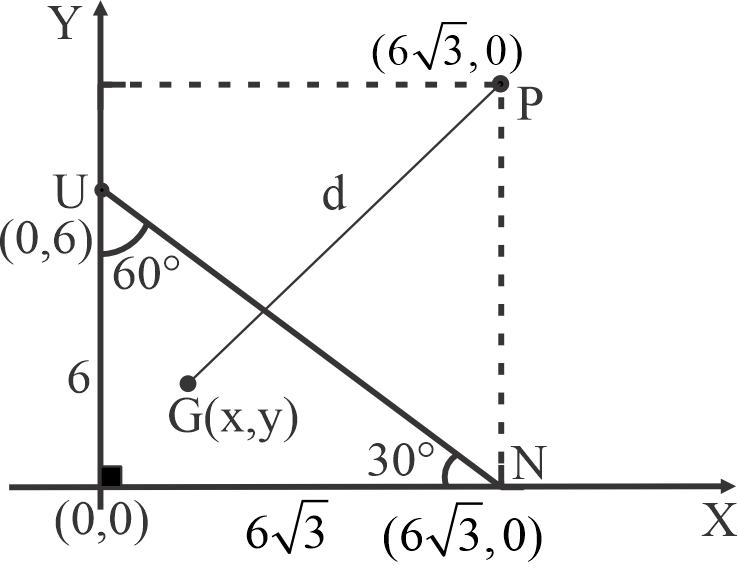
\includegraphics[width=4.5cm]{imagenes/general2024-I/etapa1/ing/geo1g24r-I.png}
		\end{minipage}
	\end{center}
	

	
		\vspace{6mm}
	
	
	
	
	
	\item En un hexágono regular ABCDEF,cuyo apotema mide $3\sqrt{3}$, calcule la medida del apotema del triángulo ACE.
	\begin{enumerate}[label=\alph*)]
		\item 3
		\item 4
		\item 6
		\item 3$\sqrt{2}$
		\item $3\sqrt{3}$
	\end{enumerate}
	
	\textbf{Respuesta correcta:} a)
	
	\vspace{2mm}
	\textbf{Solucionario:}\\[1mm]
	\begin{center}
		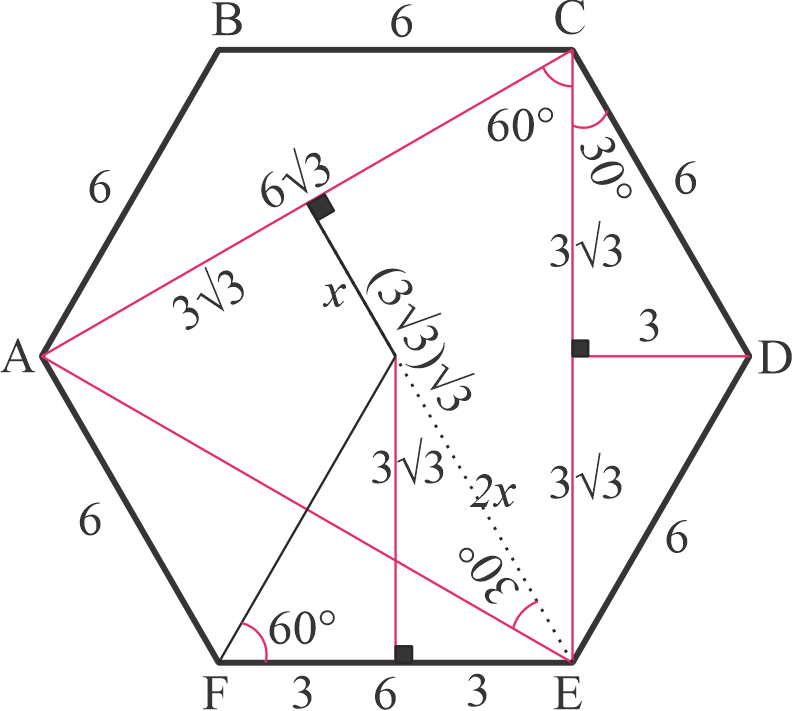
\includegraphics[width=4cm]{imagenes/general2024-I/etapa1/ing/geo2g24-I.png}
	\end{center}
	
	
	
	De la figura se tiene: $3x=9 \Rightarrow $\fbox{$x=3$}
	
	\vspace{6mm}
	
		\item En la figura, si $\alpha + \beta = 130^\circ$, calcule $x + y + z + w + v$.
		
		\begin{center}
			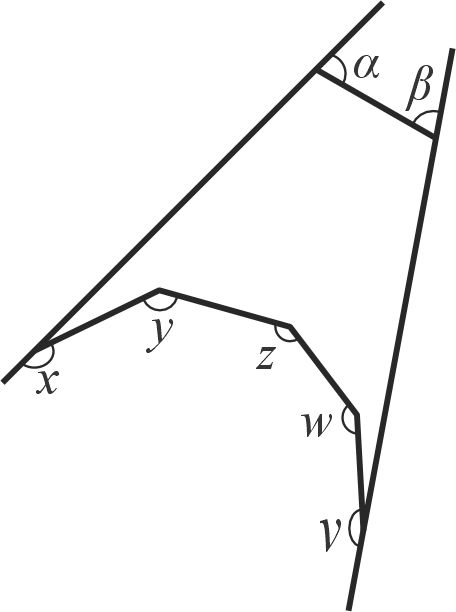
\includegraphics[width=3cm]{imagenes/general2024-I/etapa1/ing/geo3g24-I.png}
		\end{center}
		
	\begin{enumerate}[label=\alph*)]
		\item 920°
		\item 630°
		\item 860°
		\item 770°
		\item 550°
	\end{enumerate}
	
	\textbf{Respuesta correcta:} d)
	
	\vspace{2mm}
	\textbf{Solucionario:}\\[1mm]
	
	
	
		\begin{center}
		\begin{minipage}{0.45\textwidth}
		Del gráfico:\\
		$ \alpha +\beta+ a=180° \rightarrow a=50\\
		m+n+a=180° \rightarrow  m+n=130°\\
		x+y+z+w+v+m+n=180(7-2)\\
		x+y+z+w+v=180°(5)-130°\\
		x+y+z+w+v=900°-130°\\
		$\fbox{$x+y+z+w+v=770°$}
			\vspace{6mm}
		\end{minipage}
		\hfill
		\begin{minipage}{0.45\textwidth}
			\centering
			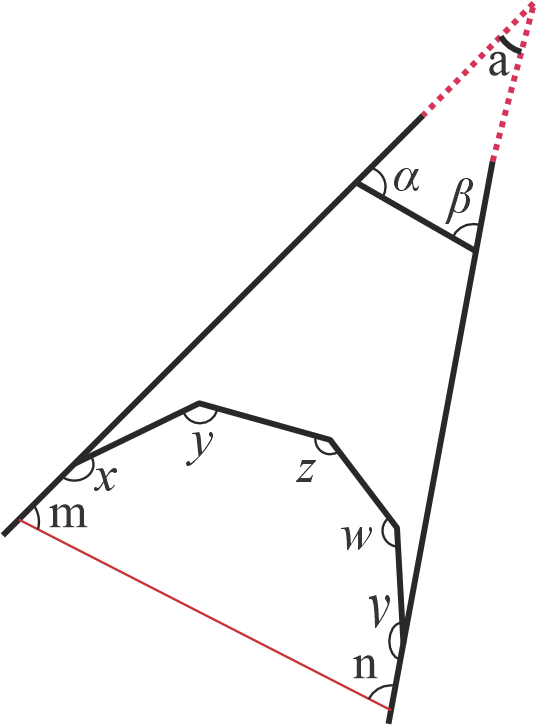
\includegraphics[width=3cm]{imagenes/general2024-I/etapa1/ing/geo3g24r-I.png}
		\end{minipage}
	\end{center}
	
	
	
	\vspace{6mm}
	
		\item Calcule el radio de la circunferencia inscrita en un trapecio rectángulo cuyas bases miden 2 y 3.
	\begin{enumerate}[label=\alph*)]
		\item $\dfrac{3}{5}$
		\item $\dfrac{6}{5}$
		\item $\dfrac{4}{3}$
		\item $\dfrac{2}{3}$
		\item $\dfrac{3}{2}$
	\end{enumerate}
	
	\textbf{Respuesta correcta:} b)
	
	\vspace{2mm}
	\textbf{Solucionario:}\\[1mm]
	\begin{center}
		\begin{minipage}{0.45\textwidth}
			Por relaciones métricas\\
			$ r^2=(2-r)(3-r)\\
			r^2=6-5r+r^2\\
			5r=6$\\
			\fbox{$4r=\dfrac{6}{5}$}
			\vspace{6mm}
		\end{minipage}
		\hfill
		\begin{minipage}{0.45\textwidth}
			\centering
			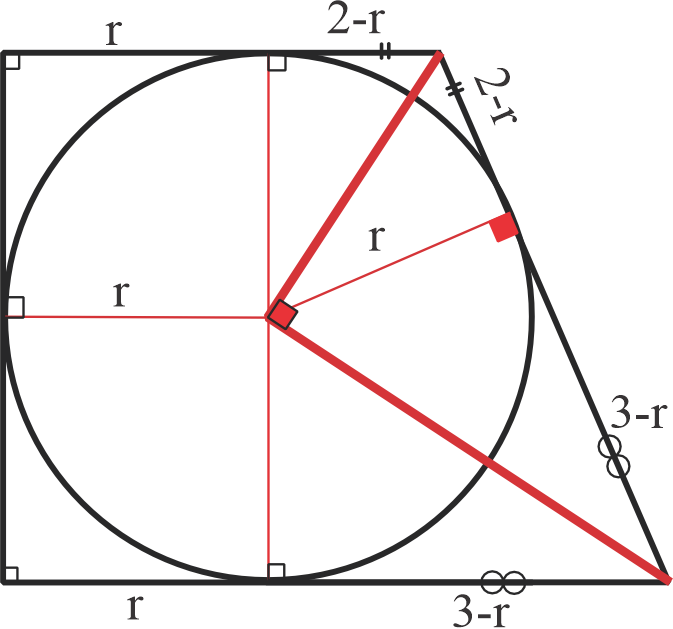
\includegraphics[width=3.8cm]{imagenes/general2024-I/etapa1/ing/geometria4g24-I.png}
		\end{minipage}
	\end{center}
	
	\vspace{6mm}
	
\end{enumerate}



\subsection*{Trigonometría}

\begin{enumerate}[resume]
	
	\item En la figura, halle $\cos 2x$
		
	\begin{center}
		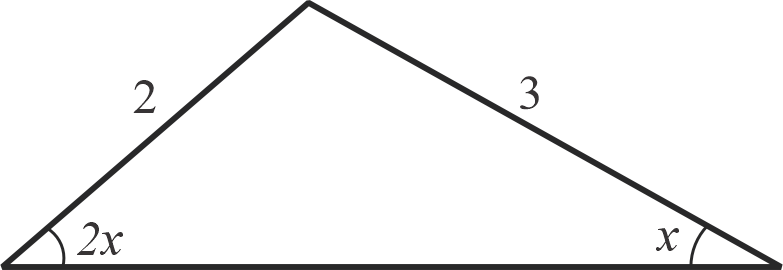
\includegraphics[width=4.5cm]{imagenes/general2024-I/etapa1/ing/trigonometria1g24-I.png}
	\end{center}
	
	\begin{enumerate}[label=\alph*)]
		\item $\displaystyle\dfrac{4}{7}$
		\item $\displaystyle\dfrac{1}{8}$
		\item $\displaystyle\dfrac{7}{8}$
		\item $\displaystyle\dfrac{\sqrt{7}}{2}$
		\item $\displaystyle\dfrac{3}{4}$
	\end{enumerate}
	
	\textbf{Respuesta correcta:} b)
	
	\vspace{2mm}
	\textbf{Solucionario:}\\[1mm]
	
	$\displaystyle\dfrac{\sen 2x}{\sen x}=\displaystyle\dfrac{3}{2}$
	
	$2 \cos x=\dfrac{3}{2}$
		
	$\cos x=\displaystyle\dfrac{3}{4}$
	
	$\cos 2x=2\cos^2x-1$
	
	$\cos 2x=2(\dfrac{3}{4})^2-1$
	
	$\cos2x=\displaystyle\dfrac{9}{8}-1$
	
	\fbox{$\cos2x=\displaystyle\dfrac{1}{8}$}
	
	\vspace{6mm}
	
	\item Halle el valor de 
	\[ M = \tan 35^\circ + \tan 25^\circ + \sqrt{3} \tan 35^\circ \cdot \tan 25^\circ \]
	
	\begin{enumerate}[label=\alph*)]
		\item1
		\item $\dfrac{1}{2}$
		\item $\dfrac{\sqrt{2}}{2}$
		\item $\dfrac{\sqrt{3}}{3}$
		\item $\sqrt{3}$
	\end{enumerate}
	
	\textbf{Respuesta correcta:} b)
	
	\vspace{2mm}
	\textbf{Solucionario:}\\[1mm]
	
	$\tan 60^\circ = \tan(35^\circ + 25^\circ) = \dfrac{\tan 35^\circ + \tan 25^\circ}{1 - \tan 35^\circ \tan 25^\circ}$ \\
	
	$\sqrt{3} = \dfrac{\tan 35^\circ + \tan 25^\circ}{1 - \tan 35^\circ \tan 25^\circ}$ \\
	
	$\sqrt{3} - \sqrt{3} \tan 35^\circ \cdot \tan 25^\circ = \tan 35^\circ + \tan 25^\circ$ \\
	$\sqrt{3} = \tan 35^\circ + \tan 25^\circ + \sqrt{3} \tan 35^\circ \cdot \tan 25^\circ$


	\vspace{6mm}
	
	\item En la figura, determine $\tan\theta + \tan \alpha$.
	
	\begin{center}
		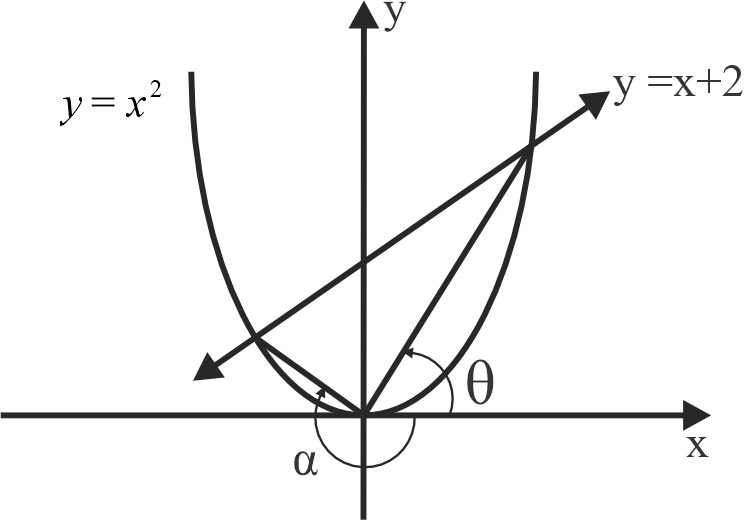
\includegraphics[width=4.3cm]{imagenes/general2024-I/etapa1/ing/trigonometria3g24-I.png}
	\end{center}
	
	
	\begin{enumerate}[label=\alph*)]
		\item 1
		\item -1
		\item 2
		\item -2
		\item -3
	\end{enumerate}
	
	\textbf{Respuesta correcta:} a)
	
	\vspace{2mm}
	\textbf{Solucionario:}\\[1mm]
	
	\begin{center}
		\begin{minipage}{0.45\textwidth}
		$y = x^2 = x + 2$ \\
		$x^2 - x - 2 = 0$ \\
		$(x - 2)(x + 1) = 0$ \\
		$x = 2 \quad x = -1$ \\
		$B(2; 4) \quad \wedge \quad A(-1; 1)$ \\
		$\tan \theta + \tan \alpha$ \\
		$= \dfrac{4}{2} + \dfrac{1}{-1}$ \\
		$= 2 - 1 = 1$
			\vspace{6mm}
		\end{minipage}
		\hfill
		\begin{minipage}{0.45\textwidth}
			\centering
			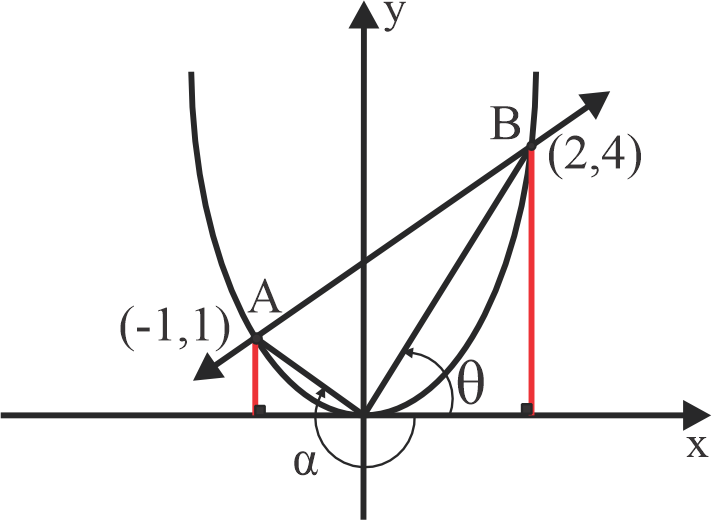
\includegraphics[width=4.3cm]{imagenes/general2024-I/etapa1/ing/trigonometria3g24r-I.png}
		\end{minipage}
	\end{center}
	
	\vspace{6mm}
	
	\item Determine el periodo de la función:\\
	$ g(x) = |\cos^4 x - \sin^4 x| $
	\begin{enumerate}[label=\alph*)]
		\item $\dfrac{\pi}{4}$
		\item $\dfrac{\pi}{2}$
		\item $\dfrac{\pi}{8}$
		\item $\dfrac{\pi}{16}$
		\item $\dfrac{3\pi}{8}$
	\end{enumerate}
	
	\textbf{Respuesta correcta:} b)
	
	\vspace{2mm}
	\textbf{Solucionario:}\\[1mm]
	
	
	\begin{center}
		\begin{minipage}{0.45\textwidth}
		$g(x) = |(\cos^2 x - \sin^2 x)(\underbrace{\cos^2 x + \sin^2 x}_{1})|$ \\
		$g(x) = |\cos^2 x - \sin^2 x|$ \\
		$g(x) = |\cos 2x|$

			\vspace{6mm}
		\end{minipage}
		\hfill
		\begin{minipage}{0.45\textwidth}
			\centering
			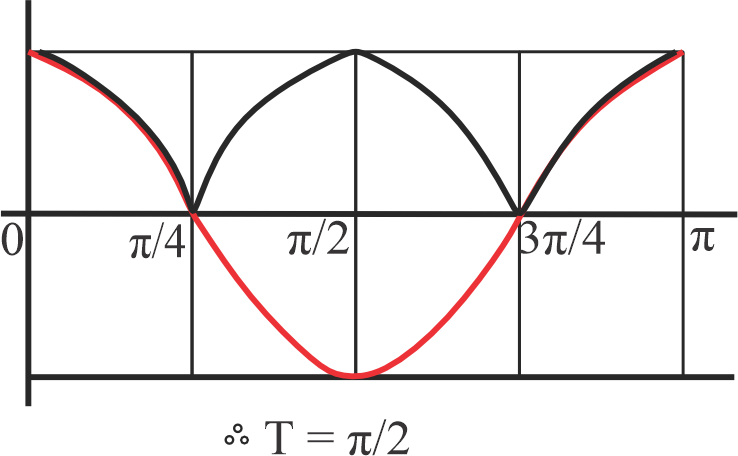
\includegraphics[width=5cm]{imagenes/general2024-I/etapa1/ing/trigonometria4g24-I.png}
		\end{minipage}
	\end{center}
	\vspace{6mm}
	
\end{enumerate}







\subsection*{Física}

\begin{enumerate}[resume]
	
	\item  Un conductor de $1 \Omega$ de resistencia se conecta a una fuente cuyo voltaje varía con el tiempo de acuerdo a la función $\varepsilon = (14 + 2t)V$, donde $t$ está en segundos. ¿Qué cantidad de carga pasa por el conductor en los 3 primeros segundos?

	\begin{enumerate}[label=\alph*)]
		\item 51 C
		\item 50 C
		\item 49 C
		\item 48 C
		\item 52 C
	\end{enumerate}
	
	\textbf{Respuesta correcta:} a)
	
	\vspace{2mm}
	\textbf{Solucionario:}\\[1mm]
	
		\begin{center}
		\begin{minipage}{0.45\textwidth}
			$V = i \cdot R \Rightarrow \varepsilon = i \cdot R$ \\
			$(14 + 2t) = i(1)$ \\
			$i = 14 + 2t$ \\
			Si $t = 0s \Rightarrow i(0) = 14 A$ \\
			Si $t = 3s \Rightarrow i(3) = 14 + 2(3) = 20 A$
			$i = \dfrac{q}{t} \rightarrow q = i \cdot t = \left( \dfrac{14 + 20}{2} \right)(3)$ \\
			$q = (17)(3) = 51 C$
			
			\vspace{6mm}
		\end{minipage}
		\hfill
		\begin{minipage}{0.45\textwidth}
			\centering
			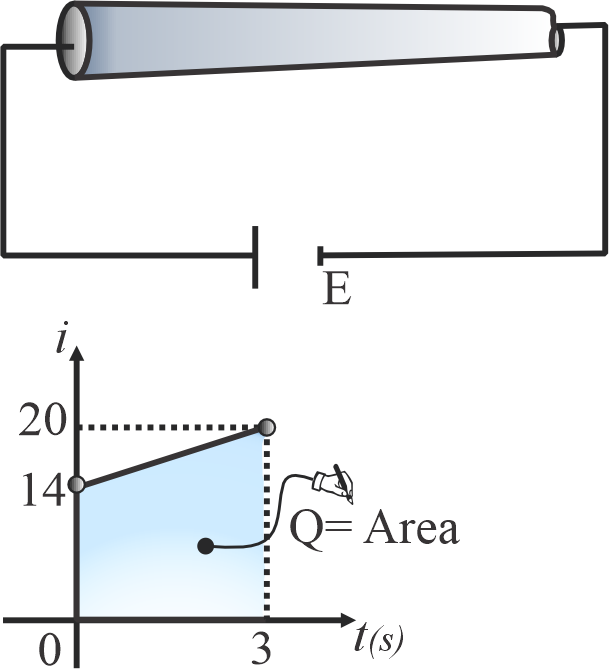
\includegraphics[width=4cm]{imagenes/general2024-I/etapa1/ing/fisica1g24-I .png}
		\end{minipage}
	\end{center}
	\vspace{6mm}
	
	\item Dos esferas de igual Volumen tienen pesos de 10N y 50N respectivamente, se encuentran en el agua flotando unidas mediante un resorte como se muestra en la figura. Halle la deformacion del resorte . (K=5N/cm)
	\begin{center}
		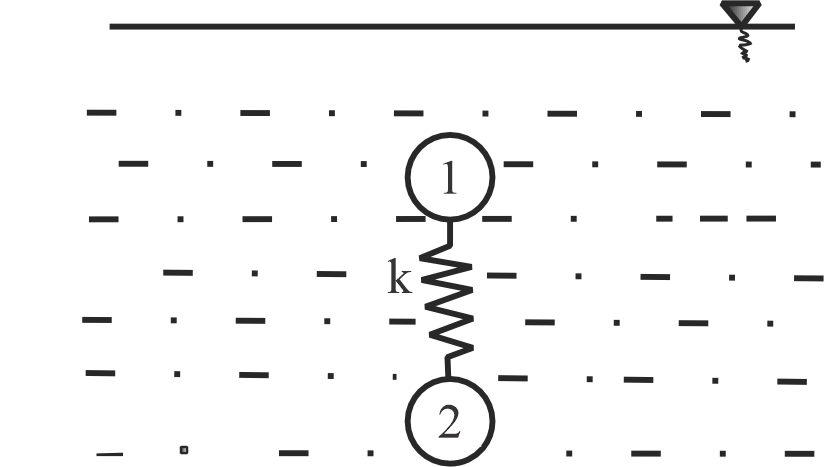
\includegraphics[width=4.5cm]{imagenes/general2024-I/etapa1/ing/fisica2g24-I.png}
	\end{center}
	
	
	\begin{enumerate}[label=\alph*)]
		\item 5 cm
		\item 4 cm
		\item 3 cm
		\item 2 cm
		\item 1 cm
	\end{enumerate}
	
	\textbf{Respuesta correcta:} b)
	
	\vspace{2mm}
	\textbf{Solucionario:}\\[1mm]
	
	\begin{center}
		\begin{minipage}{0.45\textwidth}
			\centering
		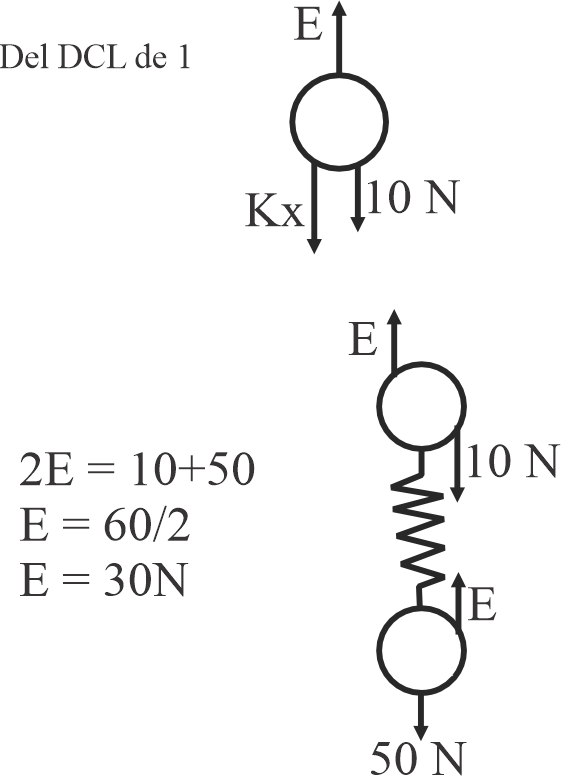
\includegraphics[width=4cm]{imagenes/general2024-I/etapa1/ing/fisica2g24r-I.png}
			
			\vspace{6mm}
		\end{minipage}
		\hfill
		\begin{minipage}{0.45\textwidth}
			$E=Kx+10\\
			x=\dfrac{E-10}{K}.............(*)\\$
			Remplazando E en (*)\\
			$x=\dfrac{30-10(N)}{5N/cm}\\
			x=4cm$\\	
		\end{minipage}
	\end{center}
	
	\vspace{6mm}
	
	
	\item Una hervidora eléctrica de $420 \, W$ se emplea para hacer hervir $1 \, kg$ de agua. Si inicialmente la temperatura del agua es de $10^\circ C$ y el agua hierve a $90^\circ C$, ¿en cuánto tiempo se logra hervir el agua? ($1 \, cal = 4,2 \, J$)
	
	\begin{enumerate}[label=\alph*)]
		\item 820 s
		\item 840 s
		\item 810 s
		\item 800 s
		\item 799 s
	\end{enumerate}
	
	\textbf{Respuesta correcta:} d)
	
	\vspace{2mm}
	\textbf{Solucionario:}\\[1mm]
	$Q = C_e \cdot m \cdot \Delta T$ \\
	$Q = \left( 1 \, \dfrac{cal}{g \cdot ^\circ C} \right) (1000 \, g) (90 - 10) \, ^\circ C$ \\
	$Q = 80 \times 10^3 \, cal$ \\
	$Q = 8 \times 10^4 \times 4,2 \, J$ \\
	$Q = 33,6 \times 10^4 \, J$ \\
	$Q = 336 \, kJ$ \\
	
	$P = \dfrac{Q}{t} \Rightarrow t = \dfrac{Q}{P} = \dfrac{336 \, kJ}{420 \, W}$ \\
	$t = \dfrac{8 \times 10^3 \times 4,2 \times 10}{420} = 800 \, s$

	\vspace{6mm}


\item Si la longitud de un péndulo simple se incrementaría en $4 \, m$, su periodo se quintuplicaría. ¿Cuál es la longitud de dicho péndulo?

\begin{enumerate}[label=\alph*)]
	\item $1/6 \, m$
	\item $1/4 \, m$
	\item $1/5 \, m$
	\item $1/3 \, m$
	\item $1/2 \, m$
\end{enumerate}

\textbf{Respuesta correcta:} a)

\vspace{2mm}
\textbf{Solucionario:}\\[1mm]
$T = 2\pi \sqrt{\dfrac{\ell}{g}}$ \\
$5T = 2\pi \sqrt{\dfrac{\ell + 4}{g}}$ \\

Dividiendo:
$\dfrac{T}{5T} = \dfrac{2\pi \sqrt{\dfrac{\ell}{g}}}{2\pi \sqrt{\dfrac{\ell + 4}{g}}}$ \\

$\left( \dfrac{1}{5} \right)^2 = \left( \sqrt{\dfrac{\dfrac{\ell}{g}}{\dfrac{\ell + 4}{g}}} \right)^2 = \left( \sqrt{\dfrac{\ell}{\ell + 4}} \right)^2$ \\

$\dfrac{1}{25} = \dfrac{\ell}{\ell + 4} \Rightarrow \ell + 4 = 25\ell$ \\

$4 = 24\ell$ \\

$\ell = \dfrac{4}{24} = \dfrac{1}{6} \, m$

\vspace{6mm}
\end{enumerate}



\subsection*{Química}

\begin{enumerate}[resume]
	
	
	
	
	
	\item Calcule el porcentaje de pureza de un mineral de $Fe$, si una muestra de $500 gramos$ del mineral impuro produce $12 gramos$ de hidrógeno según la siguiente reacción:
	
	$Fe_{(s)} + HCl_{(ac)} \longrightarrow FeCl_3 + H_{2(g)}$
	
	$(Fe = 56; \quad H = 1; \quad Cl = 35.5)$
	
	\begin{enumerate}[label=\alph*)]
		\item 46.4\%
		\item 44.8\%
		\item 43.8\%
		\item 48.4\%
		\item 40.4\%
	\end{enumerate}
	
	\textbf{Respuesta correcta:} b)
	
	\vspace{2mm}
	\textbf{Solucionario:}\\[1mm]
	Primero se debe balancear: \\
	$Fe_{(s)} + 3HCl_{(ac)} \rightarrow FeCl_3 + \dfrac{3}{2}H_{2(g)}$
	
	\vspace{2mm}
	\begin{tabular}{l c l}
		Si $Fe_{(s)}$ & \textemdash $\rightarrow$ & $\dfrac{3}{2} H_{2(g)}$ \\
		
		
		$56$ & \textemdash & $\dfrac{3}{2}(1 \times 2)$ \\
		
		$X_{Fe}$ & \textemdash & $12$ \\
	\end{tabular}
	
	\vspace{2mm}
	$X_{Fe} = 224g$
	
	\vspace{4mm}
	Determinando la pureza: \\
	Pureza $= \dfrac{Masa \: sustancia \: pura \: Fe}{Masa \: del \: mineral \: Fe} \times 100$ \\
	
	Pureza $= \dfrac{224g}{500g} \times 100$ \\
	Pureza $= 44.8\%$
	
	\vspace{6mm}
	
	
	
	\item ¿Qué cantidad de energía en joule se libera cuando se transforma en su totalidad, $5g$ de materia?
	
	\begin{enumerate}[label=\alph*)]
		\item $45 \times 10^{16}$
		\item $4,5 \times 10^{14}$
		\item $45 \times 10^{12}$
		\item $4,5 \times 10^{15}$
		\item $4,5 \times 10^{16}$
	\end{enumerate}
	
	\textbf{Respuesta correcta:} b)
	
	\vspace{2mm}
	\textbf{Solucionario:}\\[1mm]
	\textbf{datos} \\
	$E = ?$ J \\
	$m = 5g$ \\
	$c = 3 \times 10^8 m/s$\\

	$E = mc^2$ \\
	$E = 5 \times 10^{-3} kg * (3 \times 10^8 m/s)^2$ \\
	$E = 5 \times 10^{-3} * 9 \times 10^{16}$ \\
	$E = 45 \times 10^{13} J$ \\
	$E = 4,5 \times 10^{14} J.$
	
	\vspace{6mm}
	
	\item Indique Verdadero (V) o Falso (F) a las siguientes proposiciones, según corresponda:
	
	I. El ácido clorhídrico es uno de los componentes de la lluvia ácida.
	
	II. En una zona urbana debe generarse más lluvia ácida que en una zona rural.
	
	III. Un combustible con alto contenido de azufre es un promotor de la lluvia ácida.
	
	\begin{enumerate}[label=\alph*)]
		\item FFV
		\item VVF
		\item FVV
		\item FVF
		\item VFV
	\end{enumerate}
	
	\textbf{Respuesta correcta:} a)
	
	\vspace{2mm}
	\textbf{Solucionario:}\\[1mm]

	Los componentes de la lluvia ácida son los ácidos azufre y nitrógeno como $H_2SO_4$ (ácido sulfúrico) y $HNO_3$ (ácido nítrico).
	
	Los gases producidos como el $NO_x$ y $SO_x$ causan la lluvia ácida.
	
	\vspace{6mm}
	
	\item Se tiene $150g$ de una disolución que contiene $6\%$ de cierta sal, y se requiere reducir al $5\%$, ¿Qué cantidad de agua se debe añadir?
	
	\begin{enumerate}[label=\alph*)]
		\item 25 g
		\item 30g
		\item 20 g
		\item 35 g
		\item 40 g
	\end{enumerate}
	
	\textbf{Respuesta correcta:} b)
	
	\vspace{2mm}
	\textbf{Solucionario:}\\[1mm]

	DATOS \\
	$m_1 = 150g$ disolución \\
	$C_1 = 6\%$ \\
	$C_2 = 5\%$ \\
	$m_2 = m_1 + x$
	
	\vspace{2mm}
	$\Rightarrow C_1 \cdot M_1 = C_2 \cdot M_2$ \\
	$6\% (150) = 5\% (m_1 + x)$ 
	
	$\dfrac{6}{100} (150) = \dfrac{5}{100} (150 + x)$ 
	
	$900 = 750 + 5x$ \\
	$x = 30g$
	
	\vspace{6mm}
	
\end{enumerate}








\subsection*{Biología y Anatomía}

\begin{enumerate}[resume]

	\item La unidad de conservación que protege en forma intangible una especie o una comunidad determinada de plantas y/o animales, así como las formaciones naturales de interés científico y paisajístico, se denomina:
	
	\begin{enumerate}[label=\alph*)]
		\item Parque nacional.
		\item Reserva nacional.
		\item Santuario histórico.
		\item Reserva comunal.
		\item Santuario nacional.
	\end{enumerate}
	
	\textbf{Respuesta correcta:} e)
	
	\vspace{2mm}
	\textbf{Solucionario:}\\[1mm]
	Los Santuarios Nacionales son áreas de carácter intangible destinadas a proteger especies específicas de la flora y fauna, así como formaciones naturales únicas. A diferencia de los Parques Nacionales que protegen ecosistemas amplios, el Santuario se enfoca en comunidades o especies determinadas.
	
	\vspace{6mm}
	
	\item La fermentación alcohólica en la célula se realiza a nivel de:
	
	\begin{enumerate}[label=\alph*)]
		\item citosol
		\item matriz mitocondrial
		\item membrana externa mitocondrial
		\item cresta mitocondrial
		\item cloroplasto
	\end{enumerate}
	
	\textbf{Respuesta correcta:} a)
	
	\vspace{2mm}
	\textbf{Solucionario:}\\[1mm]
	La fermentación (tanto alcohólica como láctica) es un proceso anaeróbico que ocurre íntegramente en el citosol (citoplasma) de la célula. A diferencia de la respiración celular aeróbica, no requiere de las mitocondrias para la obtención de energía (ATP).
	
	\vspace{6mm}
\end{enumerate}




\subsection*{Psicología y Filosofía}

\begin{enumerate}[resume]
	
	
	\item La profesora utiliza láminas de colores para que los estudiantes puedan prestar atención durante toda la clase. Es una característica de la atención:
	
	\begin{enumerate}[label=\alph*)]
		\item direccional.
		\item selectiva.
		\item distributiva.
		\item constante.
		\item intencional.
	\end{enumerate}
	
	\textbf{Respuesta correcta:} a)
	
	\vspace{2mm}
	\textbf{Solucionario:}\\[1mm]
	La atención direccional se refiere a la capacidad de orientar los recursos sensoriales y cognitivos hacia un estímulo específico que destaca en el entorno (en este caso, las láminas de colores) para facilitar el procesamiento de la información.
	
	\vspace{6mm}
	
	\item Juan Victor desea aprender a bailar por eso práctica semanalmente. Este es un tipo de aprendizaje:
	
	\begin{enumerate}[label=\alph*)]
		\item afectivo.
		\item cognositivo.
		\item motor.
		\item social.
		\item actitudinal.
	\end{enumerate}
	
	\textbf{Respuesta correcta:} c)
	
	\vspace{2mm}
	\textbf{Solucionario:}\\[1mm]
	El aprendizaje motor involucra la adquisición de habilidades que requieren coordinación muscular, destreza física y ejecución de movimientos complejos. La práctica semanal del baile es un ejemplo clásico de cómo se automatizan estas secuencias motoras.
	
	\vspace{6mm}
	
	\item El relato ficticio que intenta explicar un aspecto de la realidad se denomina:
	
	\begin{enumerate}[label=\alph*)]
		\item filosofía.
		\item ciencia.
		\item mito.
		\item metafísica.
		\item poesía.
	\end{enumerate}
	
	\textbf{Respuesta correcta:} c)
	
	\vspace{2mm}
	\textbf{Solucionario:}\\[1mm]
	El mito es una narración tradicional y ficticia, protagonizada a menudo por seres sobrenaturales, que busca dar una explicación simbólica u ontológica a fenómenos de la naturaleza o aspectos de la condición humana antes del surgimiento del pensamiento racional-científico.
	
	\vspace{6mm}
	
	\item Si José es un sismólogo que se encarga de tomar nota de todos los detalles de los movimientos telúricos que azotan al Perú, está cumpliendo con la función ... de la ciencia.
	
	\begin{enumerate}[label=\alph*)]
		\item explicativa
		\item aplicativa
		\item social
		\item descriptiva
		\item predictiva
	\end{enumerate}
	
	\textbf{Respuesta correcta:} d)
	
	\vspace{2mm}
	\textbf{Solucionario:}\\[1mm]
	La función descriptiva de la ciencia consiste en registrar, organizar y detallar las características o propiedades de un objeto o fenómeno de estudio. Al "tomar nota de todos los detalles", el sismólogo está respondiendo a la pregunta "¿cómo es?" el fenómeno observado.
	
	\vspace{6mm}
	
\end{enumerate}



\vspace{6mm}



\subsection*{Geografía}

\begin{enumerate}[resume]
	
\item A la relación que existe entre las dimensiones del terreno y las dimensiones que se registran de ese terreno en un mapa, se denomina:

\begin{enumerate}[label=\alph*)]
	\item Proyección cartográfica
	\item Coordenada geográfica
	\item Curva de nivel
	\item Escala cartográfica
	\item Latitud y longitud
\end{enumerate}

\textbf{Respuesta correcta:} d)

\vspace{2mm}
\textbf{Solucionario:}\\[1mm]
La escala cartográfica es la relación matemática que existe entre las dimensiones reales del territorio y las dimensiones representadas en el mapa. Permite calcular distancias reales a partir de una representación reducida.

\vspace{6mm}

\item El fenómeno que eleva la temperatura de la costa norte y avanza hacia el sur del Perú, se llama:

\begin{enumerate}[label=\alph*)]
	\item Corriente de Humbolt
	\item Anticiclón del Pacífico sur
	\item Corriente de El Niño
	\item Anticiclón del Atlántico sur
	\item Corriente peruana
\end{enumerate}

\textbf{Respuesta correcta:} c)

\vspace{2mm}
\textbf{Solucionario:}\\[1mm]
La Corriente de El Niño consiste en la llegada de masas de agua cálida procedentes del norte hacia las costas peruanas. Este fenómeno provoca un aumento anómalo de la temperatura del mar y del aire en la costa norte, extendiéndose ocasionalmente hacia el sur.

\vspace{6mm}	
	
\end{enumerate}


\subsection*{Historia}

\begin{enumerate}[resume]
	
\item La arquitectura \_\_\_\_\_\_\_\_\_\_\_\_\_\_\_ apareció en el siglo XII y perduró hasta fines del XV, sus principales características fueron la ojiva o bóveda elíptica, el arco quebrado o en punta de lanza, las columnas finas y los vitrales.

\begin{enumerate}[label=\alph*)]
	\item medieval
	\item gótica
	\item románica
	\item renacentista
	\item barroca
\end{enumerate}

\textbf{Respuesta correcta:} b)

\vspace{2mm}
\textbf{Solucionario:}\\[1mm]
La arquitectura gótica es el estilo predominante en la Baja Edad Media. Sus innovaciones técnicas, como el arco apuntado (ojiva) y la bóveda de crucería, permitieron construir edificios mucho más altos y con grandes ventanales adornados con vitrales, diferenciándose del estilo románico, que era más robusto y oscuro.

\vspace{6mm}

\item Tras la renuncia del Ing. Alberto Fujimori, el Dr. Valentín Paniagua ocupa la presidencia del Perú entre el 2000 y 2001. Asumió dicho cargo a partir de su condición de

\begin{enumerate}[label=\alph*)]
	\item congresista de la República.
	\item primer ministro del gobierno.
	\item embajador ante la ONU.
	\item candidato electo.
	\item presidente del Congreso de la República.
\end{enumerate}

\textbf{Respuesta correcta:} e)

\vspace{2mm}
\textbf{Solucionario:}\\[1mm]
Tras la crisis política del año 2000 y la vacancia de la presidencia y las vicepresidencias, la línea de sucesión constitucional estableció que el cargo debía ser asumido por el Presidente del Congreso. Valentín Paniagua, quien ocupaba dicha posición en ese momento, asumió la presidencia de un gobierno de transición para convocar a nuevas elecciones.

\vspace{6mm}	
	
\end{enumerate}




\subsection*{Educación Cívica}

\begin{enumerate}[resume]
	
	\item Según la estructura jerárquica del sistema jurídico normativo del Perú, los decretos supremos, los edictos municipales y los decretos regionales ejecutivos, corresponden al:
	
	\begin{enumerate}[label=\alph*)]
		\item I nivel — constitucional.
		\item II nivel — legal.
		\item III nivel — reglamentario.
		\item IV nivel — resoluciones.
		\item V nivel — normas de interés particular.
	\end{enumerate}
	
	\textbf{Respuesta correcta:} c)
	
	\vspace{2mm}
	\textbf{Solucionario:}\\[1mm]
	En la pirámide de Kelsen aplicada al sistema peruano, el tercer nivel (nivel reglamentario) agrupa normas de carácter administrativo general emitidas por el Ejecutivo y gobiernos locales. Los decretos supremos y edictos municipales reglamentan las leyes de jerarquía superior sin contravenirlas.
	
	\vspace{6mm}
	
	\item Según Karl Loewenstein, bajo el sistema político del constitucionalismo, un tipo de democracia constitucional es:
	
	\begin{enumerate}[label=\alph*)]
		\item el nacional — socialismo alemán.
		\item el comunismo chino.
		\item la democracia popular.
		\item la democracia directa.
		\item el neopresidencialismo.
	\end{enumerate}
	
	\textbf{Respuesta correcta:} d)
	
	\vspace{2mm}
	\textbf{Solucionario:}\\[1mm]
	Karl Loewenstein clasifica los sistemas según el ejercicio del poder. En el marco del constitucionalismo, donde el poder está limitado y controlado, la democracia directa se considera una forma pura de democracia constitucional donde la soberanía reside y es ejercida sin intermediarios por el pueblo dentro de un orden jurídico establecido.
	
	\vspace{6mm}
	
\end{enumerate}


\vspace{6mm}


\subsection*{Economía}

\begin{enumerate}[resume]
	
	\item La toma de decisiones de un productor con el objetivo de maximizar sus beneficios, es campo de estudio de la ...
	
	\begin{enumerate}[label=\alph*)]
		\item macroeconomía.
		\item microeconomía.
		\item política económica.
		\item economía política.
		\item economía normativa.
	\end{enumerate}
	
	\textbf{Respuesta correcta:} b)
	
	\vspace{2mm}
	\textbf{Solucionario:}\\[1mm]
	La microeconomía estudia el comportamiento individual de los agentes económicos, como consumidores y empresas (productores). El análisis de cómo un productor decide niveles de producción y costos para maximizar su utilidad es un tema central de esta rama.
	
	\vspace{6mm}
	
	\item En relación a las exportaciones de la economía Peruana se puede afirmar que se ...
	
	\begin{enumerate}[label=\alph*)]
		\item venden maquinarias y equipos.
		\item concentra en productos no tradicionales.
		\item elaboran productos con mucho valor agregado.
		\item concentra en el oro, el cobre y la harina de pescado.
		\item concentra en productos tradicionales con mucho valor agregado.
	\end{enumerate}
	
	\textbf{Respuesta correcta:} d)
	
	\vspace{2mm}
	\textbf{Solucionario:}\\[1mm]
	La estructura exportadora del Perú es primario-exportadora. Esto significa que la mayor parte de las divisas provienen de productos tradicionales (materias primas con bajo valor agregado), destacando principalmente los minerales como el oro y el cobre, además de la harina de pescado.
	
	\vspace{6mm}
	
\end{enumerate}


\subsection*{Comunicación}

\begin{enumerate}[resume]
	
\item La computadora es la consecuencia de muchos inventos del hombre para hacer más fácil los cálculos matemáticos, la composición de textos, el diseño de gráficos, etc.
En el texto, ¿Qué tipo de coma se utiliza?

\begin{enumerate}[label=\alph*)]
	\item coma elíptica
	\item coma apositiva
	\item coma enfática
	\item coma enumerativa
	\item coma explicativa
\end{enumerate}

\textbf{Respuesta correcta:} d)

\vspace{2mm}
\textbf{Solucionario:}\\[1mm]
La coma enumerativa se utiliza para separar elementos análogos dentro de una serie o lista. En el texto, se emplea para separar las distintas funciones de la computadora: "...cálculos matemáticos, la composición de textos, el diseño de gráficos...".

\vspace{6mm}

\item Los seres vivos que existen en nuestro planeta pueden clasificarse de acuerdo a la forma como obtienen sus alimentos. Según estas características pueden ser autótrofos y heterótrofos.
¿A qué tipo de texto corresponde?

\begin{enumerate}[label=\alph*)]
	\item Descriptivo
	\item Argumentativo
	\item Narrativo
	\item Instructivo
	\item Expositivo
\end{enumerate}

\textbf{Respuesta correcta:} e)

\vspace{2mm}
\textbf{Solucionario:}\\[1mm]
El texto es expositivo porque su intención principal es informar y transmitir datos de manera objetiva sobre un tema específico (la clasificación de los seres vivos según su alimentación), sin intentar convencer al lector ni contar una historia.

\vspace{6mm}

\item El presidente del barrio San José convoca a una reunión extraordinaria y pide a su secretario tomar anotaciones del suceso.
¿Qué documento redactará el secretario?

\begin{enumerate}[label=\alph*)]
	\item Solicitud
	\item Carta
	\item Memorando
	\item Acta
	\item Oficio
\end{enumerate}

\textbf{Respuesta correcta:} d)

\vspace{2mm}
\textbf{Solucionario:}\\[1mm]
El acta es el documento oficial donde se registran de manera detallada los hechos, acuerdos y deliberaciones ocurridos durante una reunión o asamblea. Es la función específica del secretario dar fe de lo sucedido mediante este documento.

\vspace{6mm}

\item En la narración, la parte donde se presenta los personajes y el lugar de los eventos se denomina:

\begin{enumerate}[label=\alph*)]
	\item Título
	\item Inicio
	\item Nudo
	\item Desarrollo
	\item Desenlace
\end{enumerate}

\textbf{Respuesta correcta:} b)

\vspace{2mm}
\textbf{Solucionario:}\\[1mm]
El inicio (o planteamiento) es la parte inicial de una estructura narrativa. Su función es situar al lector en el contexto, presentando a los personajes principales, el tiempo y el lugar donde se desarrollará la acción antes de que aparezca el conflicto.

\vspace{6mm}
	
\end{enumerate}






\subsection*{Literatura}

\begin{enumerate}[resume]
	
	\item Los temas fundamentales que desarrolla Kafka en sus obras son:
	
	\begin{enumerate}[label=\alph*)]
		\item el capitalismo y el abuso.
		\item el caos y el absurdo.
		\item la dominación y el servilismo.
		\item la deshumanización y el amor
		\item el rechazo al mundo y el deshonor
	\end{enumerate}
	
	\textbf{Respuesta correcta:} b)
	
	\vspace{2mm}
	\textbf{Solucionario:}\\[1mm]
	Franz Kafka es el máximo exponente de la literatura del absurdo. Sus obras exploran la angustia existencial del individuo frente a situaciones caóticas, burocráticas e incomprensibles donde la lógica común no aplica, reflejando la desorientación del hombre moderno.
	
	\vspace{6mm}
	
	\item Mariano Melgar, para crear el Yaraví, tuvo como referencia al...
	
	\begin{enumerate}[label=\alph*)]
		\item haylli.
		\item lanka.
		\item haravicu.
		\item huayño
		\item harawi.
	\end{enumerate}
	
	\textbf{Respuesta correcta:} e)
	
	\vspace{2mm}
	\textbf{Solucionario:}\\[1mm]
	El Yaraví melgariano tiene su origen en el \textit{harawi} incaico, una especie lírica de tono melancólico y sentimental que expresaba el dolor por la ausencia o pérdida de la amada. Melgar asimiló esta tradición indígena y la fusionó con formas métricas españolas.
	
	\vspace{6mm}
	
\end{enumerate}







\subsection*{Razonamiento Matemático}

\begin{enumerate}[resume]
	
	\item Se tiene un reloj de agujas que a las 0:00 horas del primero de enero marcaba las 5:50 a.m. Si dicho reloj se adelanta 30 segundos cada hora, ¿Cuántas veces durante el año marcará la hora correcta?
	
	\begin{enumerate}[label=\alph*)]
		\item 4
		\item 8 
		\item 12 
		\item 2
		\item 6
	\end{enumerate}
	
	\textbf{Respuesta correcta:} e)
	
	\vspace{2mm}
	\textbf{Solucionario:}\\[1mm]
	Determinando cada cuántos días marcará la hora correcta:
	
	Para que un reloj de agujas vuelva a marcar la hora correcta, debe acumular un adelanto de 12 horas (720 minutos).
	
	\begin{itemize}
		\item Adelanta: $30s = \dfrac{1}{2}$ min $\xrightarrow{\times 2}$ en 1 h.
		\item Adelanta: 720 min $\xrightarrow{\times 2}$ en 1440 h.
	\end{itemize}
	
	Convertimos las horas a días:
	$1440 \text{ h} = \dfrac{1440}{24} = 60 \text{ días.}$
	
	$\Rightarrow$ Cada 60 días marcará la hora exacta.
	
	\vspace{2mm}
	\textbf{Para un año (365 días):}
	$\# \text{ veces} = \dfrac{365}{60} \approx 6 \text{ veces.}$
	
	\vspace{6mm}

	
	\item Si a cada uno de los 4 términos de una proporción geométrica se le quita una misma cantidad, se obtendrá 20, 28, 32 y 44. Halle la suma de los términos de la proporción.
	
	\begin{enumerate}[label=\alph*)]
		\item 140
		\item 124
		\item 144
		\item 112
		\item 104
	\end{enumerate}
	
	\textbf{Respuesta correcta:} a)
	
	\vspace{2mm}
	\textbf{Solucionario:}\\[1mm]
	La proporción: $\dfrac{a}{b} = \dfrac{c}{d} \quad \text{(I)}$
	
	Se le quita la misma cantidad:
	$\left. \begin{array}{l} 
		a - x = 20 \Rightarrow a = 20 + x \\
		b - x = 28 \Rightarrow b = 28 + x \\
		c - x = 32 \Rightarrow c = 32 + x \\
		d - x = 44 \Rightarrow d = 44 + x 
	\end{array} \right\} \text{(II)}$
	
	Se tendrá que:\\
	$a + b + c + d = 124 + 4x \quad \text{(III)}$
	
	Remplazando (II) en (I) y resolviendo:
	$$\dfrac{20 + x}{28 + x} = \dfrac{32 + x}{44 + x} \Rightarrow 880 + 64x + x^2 = 896 + 60x + x^2$$
	$4x = 16 \Rightarrow x = 4$
	
	Se pide $a + b + c + d = ?$\\
	De (III): $a + b + c + d = 124 + 4(4) = 140$
	
	\vspace{6mm}


\item En un pastizal, una vaca es atada a una estaca con una cuerda de 4 metros. Comiendo la misma cantidad de pasto diario, consumió todo lo que estaba a su alcance en 4 días. Si luego se aumenta 4 metros más de cuerda, ¿cuántos días más se demorará en consumir el pasto restante?

\begin{enumerate}[label=\alph*)]
	\item 9 días
	\item 16 días
	\item 12 días
	\item 18 días
	\item 8 días
\end{enumerate}

\textbf{Respuesta correcta:} c)

\vspace{4mm}
\textbf{Solucionario:}\\[1mm]



\begin{center}
	\begin{minipage}{0.45\textwidth}
		El área que consume la vaca es un círculo: $A = \pi \cdot r^2$.\\

		\textbf{Caso 1 ($r = 4$ m):}\\
		$A_1 = \pi(4)^2 = 16\pi$\\
		Relacionamos días y área:\\
		$4 \text{ días} \longrightarrow 16\pi$\\
		
		\textbf{Caso 2 ($r = 8$ m):}\\
		El área nueva es la corona circular\\ 
		(el pasto restante):\\
		$A_{restante} = \pi(8)^2 - \pi(4)^2$\\
		$A_{restante} = 64\pi - 16\pi = 48\pi$\\
		
		\textbf{Regla de tres:}\\
		$\dfrac{x}{4} = \dfrac{48\pi}{16\pi} \implies x = 4 \cdot 3 = 12$\\
		
		\textbf{Demora 12 días más.}\\
	\end{minipage}
	\hfill
	\begin{minipage}{0.45\textwidth}
		\centering
		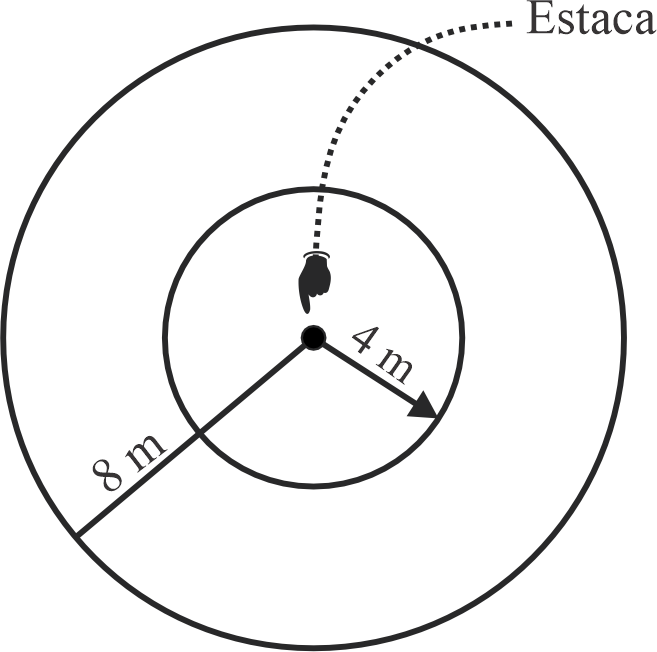
\includegraphics[width=3.5cm]{imagenes/general2024-I/etapa1/ing/RM3g24-I.png}
	\end{minipage}
\end{center}








\item Si $ABCD$ es un cuadrado de lado $4$ m, calcule el perímetro de la región sombreada.

\begin{center}
	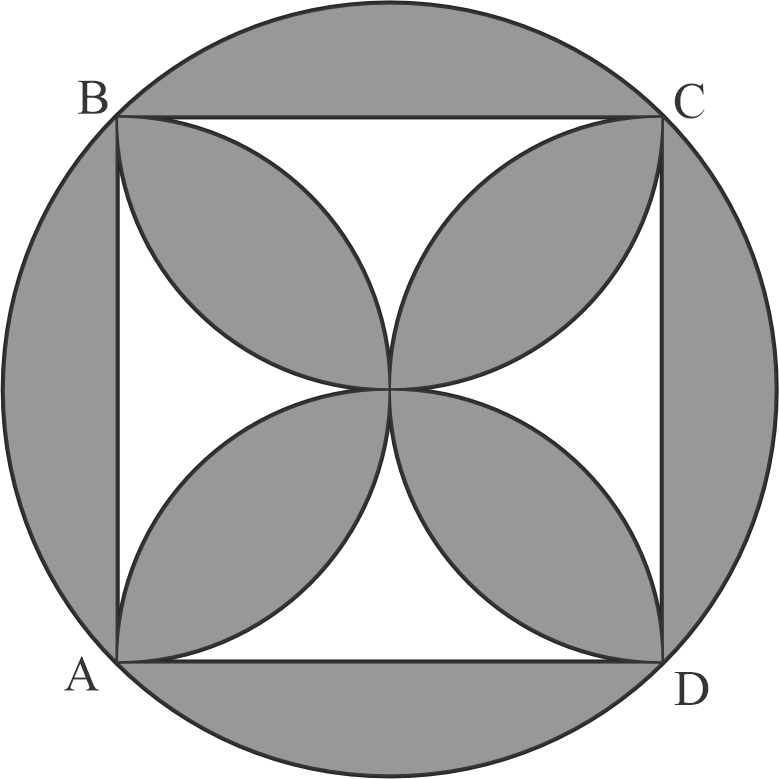
\includegraphics[width=3.5cm]{imagenes/general2024-I/etapa1/ing/RM4g24-I.png} % Ajusta el nombre según tu archivo
\end{center}

\begin{enumerate}[label=\alph*)]
	\item $4(\pi + 2\pi + 4)$ m
	\item $4(\sqrt{2}\pi + 2\pi + 4)$ m
	\item $4(2\sqrt{2}\pi + \pi + 4)$ m
	\item $8(2\sqrt{2}\pi + 2\pi + 2)$ m
	\item $8(4\sqrt{2}\pi + \pi + 2)$ m
\end{enumerate}

\textbf{Respuesta correcta:} b)

\vspace{4mm}
\textbf{Solucionario:}\\[1mm]


\begin{center}
	\begin{minipage}{0.45\textwidth}
		\item[i)] \textbf{Del Grafico}\\
		\item[ii)] \textbf{Perimetro cuadrado}\\
		$= 16 \text{ m}$\\
		\item[iii)] \textbf{Circunferencia}\\
		$P = 2\pi r = 2\pi (2\sqrt{2}) = 4\sqrt{2}\pi$\\
		$\text{perimetro arcos} \left( \begin{array}{l} 
			\stackrel{\frown}{AB} = 2\pi \\
			\stackrel{\frown}{CD} = 2\pi \\
			\stackrel{\frown}{BC} = 2\pi \\
			\stackrel{\frown}{AD} = 2\pi 
		\end{array} \right. = 8\pi$
		
		\vspace{4mm}
		$\therefore \textbf{perímetro} = (4\sqrt{2}\pi + 8\pi + 16)m$ \\
		\hspace{20mm} $= 4(\sqrt{2}\pi + 2\pi + 4)m$
		
	\end{minipage}
	\hfill
	\begin{minipage}{0.45\textwidth}
		\centering
		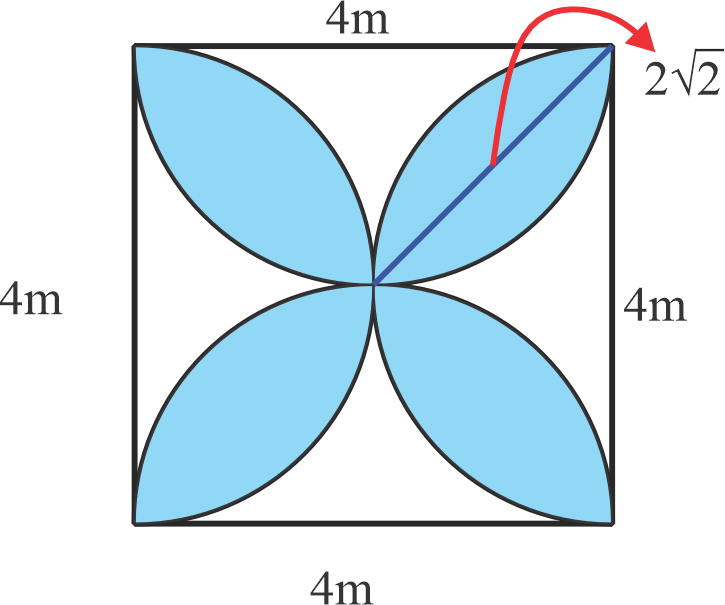
\includegraphics[width=4cm]{imagenes/general2024-I/etapa1/ing/RM4g24r-I.png} 
	\end{minipage}
\end{center}

	\item Se define el operador:
	$$2a^b \circledast 3b^a = \sqrt{a^2 + b^2}$$
	Halle: $128 \circledast 243$
	
	\begin{enumerate}[label=\alph*)]
		\item 5
		\item 3
		\item 4
		\item 7
		\item 6
	\end{enumerate}
	
	\textbf{Respuesta correcta:} a)
	
	\vspace{2mm}
	\textbf{Solucionario:}\\[1mm]
	Dando la forma de la definición:\\
	$$128 \circledast 243 = 2 \cdot 4^3 \circledast 3 \cdot 3^4$$\\
	De donde se obtiene que:\\
	$a = 4$ y $b = 3$\\
	
	Remplazando:\\
	$\Rightarrow \sqrt{4^2 + 3^2}$\\
	$= \sqrt{16 + 9} = \sqrt{25} = 5$\\
	
	\vspace{6mm}


	\item Calcule la suma:
	$$S = 25 + 36 + 49 + \dots + 400$$
	
	\begin{enumerate}[label=\alph*)]
		\item 2810
		\item 2820
		\item 2830
		\item 2840
		\item 2850
	\end{enumerate}
	
	\textbf{Respuesta correcta:} d)
	
	\vspace{2mm}
	\textbf{Solucionario:}\\[1mm]
	\underline{(Fórmula)}
	$$\sum_{i=1}^{n} i^2 = \dfrac{n(n+1)(2n+1)}{6}$$
	
	Identificando los términos de la serie:
	$$S = \sum_{i=1}^{20} i^2 - \sum_{i=1}^{4} i^2 = (1^2 + 2^2 + 3^2 + \dots + 20^2) - (1^2 + 2^2 + 3^2 + 4^2)$$
	
	Aplicando la fórmula para $n=20$ y $n=4$:
	$$= \dfrac{20(20+1)(2(20)+1)}{6} - \dfrac{4(4+1)(2(4)+1)}{6}$$
	$$= 2870 - 30$$
	$$= 2840$$
	
	\vspace{6mm}
	
	
\end{enumerate}





\subsection*{Razonamiento Verbal}

\begin{enumerate}[resume]
	
	\item La palabra ingeniero proviene del latín \textit{ingenium} que significa:
	
	\begin{enumerate}[label=\alph*)]
		\item Poseer o estimular la capacidad de creación, invención, etc.
		\item Adaptarse frente a un agente perturbador, estado o situación adverso.
		\item Discurrir o inventar con prontitud y facilidad.
		\item Emprender con resolución, acciones o empresas innovadoras.
		\item Poseer los conocimientos especiales de una ciencia o arte.
	\end{enumerate}
	
	\textbf{Respuesta correcta:} c)
	
	\vspace{2mm}
	\textbf{Solucionario:}\\[1mm]
	Etimológicamente, \textit{ingenium} se refiere a la cualidad natural de una persona para crear o dar soluciones ingeniosas. La definición que mejor se ajusta a esta raíz es la capacidad de discurrir o inventar de manera rápida y eficaz ante un desafío.
	
	\vspace{6mm}
	
	\item Complete la oración:
	
	No logró ingresar a la universidad \_\_\_\_\_\_\_ de haberse preparado adecuadamente, \_\_\_\_\_\_\_, su perseverancia será recompensada en algún momento.
	
	\begin{enumerate}[label=\alph*)]
		\item no obstante \textemdash por lo tanto
		\item a pesar \textemdash sin embargo
		\item luego \textemdash por lo que
		\item después \textemdash entonces
		\item empero \textemdash pero
	\end{enumerate}
	
	\textbf{Respuesta correcta:} b)
	
	\vspace{2mm}
	\textbf{Solucionario:}\\[1mm]
	El primer espacio requiere un conector concesivo ("a pesar") que indique que el resultado fue adverso pese a la preparación. El segundo espacio requiere un conector adversativo ("sin embargo") para introducir la idea de esperanza en la perseverancia futura.
	
	\vspace{6mm}
	
	\item Encuentre la oración a eliminar:
	
	I. La situación económica del Perú es el resultado de borrones y cuentas nuevas en la política peruana. \\
	II. Cada nueva administración gubernamental trata de desaparecer los vestigios de la anterior. \\
	III. De lo que se trata es concertar un proyecto de desarrollo que todos los partidos respeten. \\
	IV. De este modo se podrá planificar para el futuro programas de mediano y largo plazo. \\
	V. La concentración es básicamente un nivel de acuerdo.
	
	\begin{enumerate}[label=\alph*)]
		\item IV
		\item II
		\item V
		\item I
		\item III
	\end{enumerate}
	
	\textbf{Respuesta correcta:} c)
	
	\vspace{2mm}
	\textbf{Solucionario:}\\[1mm]
	El texto trata sobre la falta de continuidad política y la necesidad de proyectos de desarrollo a largo plazo. La oración V se elimina por impertinencia, ya que define "concentración" de forma aislada, alejándose del eje temático sobre administración pública y planificación.
	
	\vspace{6mm}
	
	\item Identifica el par analógico.
	
	SEDIMENTACIÓN : ESTRATO ::
	
	\begin{enumerate}[label=\alph*)]
		\item erosión : desgaste.
		\item ciencia : estudio.
		\item ficción : realidad.
		\item nobleza : verdad.
		\item base : capa.
	\end{enumerate}
	
	\textbf{Respuesta correcta:} e)
	
	\vspace{2mm}
	\textbf{Solucionario:}\\[1mm]
	La relación es de proceso a producto: la sedimentación genera el estrato (una capa de sedimentos). De manera análoga, una base constituye el fundamento o soporte de una capa en diversas estructuras o formaciones.
	
	\vspace{6mm}
	
	\item PLAN DE REDACCIÓN \\
	\textbf{Galileo Galilei}
	
	I. Realizó experiencias sobre la caída de los cuerpos e inventó el termómetro. \\
	II. Fue matemático, físico y astrónomo y el verdadero fundador de la Física y la Mecánica. \\
	III. A los 19 años, observó en la Catedral de Pisa, una lámpara que se balanceaba colgada de la cúpula y se le ocurrió aplicar el péndulo a la medida del tiempo. \\
	IV. Partidario del sistema de Copérnico, abjuró de sus convicciones sobre el movimiento de la tierra obligado por la inquisición. \\
	V. Por ello, Galileo es considerado como el prototipo de mártir a causa de la ciencia.
	
	\begin{enumerate}[label=\alph*)]
		\item II - I - III - IV - V
		\item II - III - IV - I - V
		\item III - II - I - IV - V
		\item III - II - I - V - IV
		\item IV - V - I - II - III
	\end{enumerate}
	
	\textbf{Respuesta correcta:} d)
	
	\vspace{2mm}
	\textbf{Solucionario:}\\[1mm]
	El orden lógico sigue un criterio cronológico y de relevancia: se inicia con su juventud (III), se define su importancia general (II), se mencionan sus inventos y experimentos (I), se concluye con el impacto de su juicio (V) y su conflicto final con la inquisición (IV).
	
	\vspace{6mm}
	
	\item Los ríos se caracterizan por su baja productividad primaria y baja concentración de oxígeno disuelto. Sin embargo, en ellos vive un gran número de poblaciones de animales debido a que la corriente del río carga materiales orgánicos de otros sistemas y ventila los organismos sosteniéndolos a pesar de las condiciones antes referidas. Aplicando el modelo producción  respiración, el río es un sistema heterotrófico, donde la respiración es mayor que la producción. La productividad primaria del río radica principalmente en la superficie de las rocas o en los lentos remansos, donde la poca velocidad de las aguas permite el crecimiento de algas o de plantas acuáticas vasculares desde el punto de vista regional los ríos transportan con rapidez materiales y energía entre un sistema y otro.
	
	Pese a sus deficientes condiciones, los ríos pueden sostener vida gracias a que:
	
	\begin{enumerate}[label=\alph*)]
		\item Son subsidiados por lagos.
		\item La agitación mecánica arrastra e incorpora al río lo necesario.
		\item El río tiene zonas tranquilas, los remansos favorables a la vida.
		\item La respiración es mayor que la producción.
		\item Los organismos se han adaptado a esas duras condiciones.
	\end{enumerate}
	
	\textbf{Respuesta correcta:} b)
	
	\vspace{2mm}
	\textbf{Solucionario:}\\[1mm]
	Según el texto, la corriente del río carga materiales orgánicos y ventila los organismos. Esta "agitación mecánica" permite la incorporación de nutrientes y oxígeno de otros sistemas, compensando la baja productividad primaria propia del río.
	
	\vspace{6mm}
	
\end{enumerate}


\subsection*{Inglés}

\begin{enumerate}[resume]

	\item Answer the question about the underline word.
	"The mothers day is \underline{in} May on the second Sunday"
	What is underline word?
	
	\begin{enumerate}[label=\alph*)]
		\item Preposition
		\item Verb
		\item Gerund
		\item Noun
		\item Simple
	\end{enumerate}
	
	\textbf{Respuesta correcta:} a)
	
	\vspace{2mm}
	\textbf{Solucionario:}\\[1mm]
	En la gramática inglesa, "in" es una preposición de tiempo que se utiliza antes de meses, años, siglos y períodos largos. En la oración proporcionada, establece la relación temporal entre el Día de la Madre y el mes de mayo.
	
	\vspace{6mm}
	
	\item Select the option with the irregular verb in the simple past tense.
	
	\begin{enumerate}[label=\alph*)]
		\item I lived to dance
		\item We live in Puno
		\item We meet en the afternoon
		\item I enjoyed singing with him
		\item I had two sisters
	\end{enumerate}
	
	\textbf{Respuesta correcta:} e)
	
	\vspace{2mm}
	\textbf{Solucionario:}\\[1mm]
	Los verbos irregulares son aquellos que no siguen la regla estándar de añadir "-ed" para formar el tiempo pasado. El verbo "had" es el pasado del verbo irregular "have". Las otras opciones utilizan verbos regulares en pasado ("lived", "enjoyed") o están en tiempo presente ("live", "meet").
	
	\vspace{6mm}
	
\end{enumerate}





\subsection*{Quechua y Aimara}

\begin{enumerate}[resume]
	
	\item Ñuqaq kimsa chunka uwihaykuna karqan, kimsata atuq mikhurqapusqa, ¿Hayk'a uwihakunataq qhipawan?/Nayaxa kimsatunka uwijaniyatwa. Kimsaru qamaqi manq'antawayi. ¿Qawqhasa jichaxa utjaski?
	
	\begin{enumerate}[label=\alph*)]
		\item Iskay chunka pichqayuq/Pä tunka phisqani.
		\item Iskay chunka suqtayuq/Pä tunka suxtani.
		\item Iskay chunka qanchisniyuq/Pä tunka paqallquni.
		\item Iskay chunka pusaqniyuq/Pä tunka kimsaqallquni.
		\item Iskay chunka isqunniyuq/Pä tunka llatunkani.
	\end{enumerate}
	
	\textbf{Respuesta correcta:} c)
	
	\vspace{2mm}
	\textbf{Solucionario:}\\[1mm]
	El problema plantea una resta básica en Quechua y Aimara: "Tenía 30 ovejas (\textit{kimsa chunka} / \textit{kimsatunka}) y el zorro se comió 3 (\textit{kimsa} / \textit{kimsa})". 
	Operación: $30 - 3 = 27$.
	En Quechua, 27 es \textit{Iskay chunka qanchisniyuq} y en Aimara es \textit{Pä tunka paqallquni}.
	
	\vspace{6mm}
	
	\item Chunkaman tawata yapaykuptiyri, ¿Hayk'ataq kanman?/Tunkaru pusimpi apxatirista, ¿Ukaxa qawqhaspasa?
	
	\begin{enumerate}[label=\alph*)]
		\item Chunka hukniyuq/Tunka mayani.
		\item Chunka iskayniyuq/Tunka payani.
		\item Chunka kimsayuq/Tunka kimsani.
		\item Chunka tawayuq/Tunka pusini.
		\item Chunka pichqayuq/Tunka phisqani.
	\end{enumerate}
	
	\textbf{Respuesta correcta:} d)
	
	\vspace{2mm}
	\textbf{Solucionario:}\\[1mm]
	La pregunta solicita realizar una suma: "A diez (\textit{chunka} / \textit{tunka}) le agrego cuatro (\textit{tawa} / \textit{pusi}), ¿cuánto sería?".
	Operación: $10 + 4 = 14$.
	En Quechua, 14 se dice \textit{Chunka tawayuq} y en Aimara se dice \textit{Tunka pusini}.
	
	\vspace{6mm}
	
\end{enumerate}

\section*{Área: Biomédicas}


\subsection*{Aritmética}

\begin{enumerate}
	
	\item Determine el esquema mólecular simplificado del siguiente circuito:
	
	
	\begin{figure}[h]
		\centering
		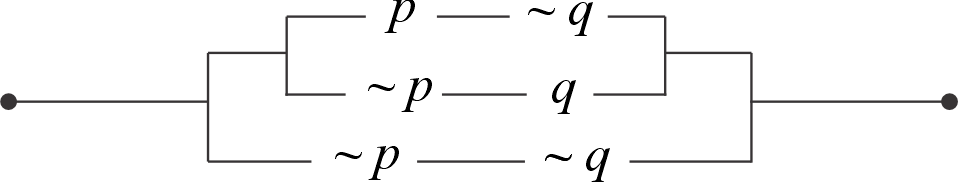
\includegraphics[width=0.6\textwidth]{imagenes/general2024-I/etapa1/bio/aritmetica1g24-I}
		%\caption{Descripción de la imagen}
		%\label{fig:ejemplo}
	\end{figure}
	
	
	
	
	\begin{enumerate}[label=\alph*)]
		\item $p \land q$
		\item $p \lor q$
		\item $\sim p\,\,\land \sim q$
		\item $\sim p\,\,\lor \sim q$
		\item $\sim p\,\land q$
	\end{enumerate}
	
	\textbf{Respuesta correcta:} d)
	
	\vspace{2mm}
	\textbf{Solucionario:}\\[1mm]
	Del circuito inicial podemos formar lo siguiente, reduciendo:
	
	\begin{figure}[h]
		\centering
		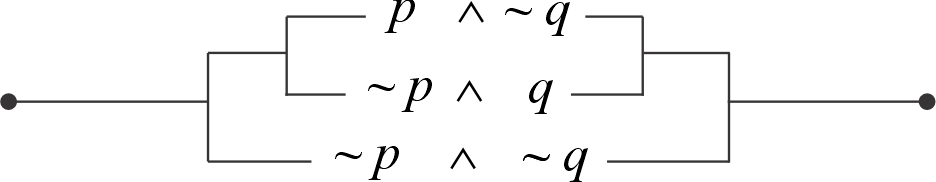
\includegraphics[width=0.6\textwidth]{imagenes/general2024-I/etapa1/bio/aritmetica1soluciong24-I}
		%\caption{Descripción de la imagen}
		%\label{fig:ejemplo}
	\end{figure}
	
	
	De ahí tendremos la siguiente expresión lógica:
	
	\[\begin{array}{l}
		\equiv [(p \,\wedge  \sim q) \vee ( \sim p \wedge q)] \vee ( \sim p \wedge  \sim q)\\
		\equiv [(p \vee ( \sim p \wedge q)) \wedge ( \sim q \vee ( \sim p \wedge q))] \vee  \sim (p \wedge q)\\
		\equiv [(p \vee q) \wedge ( \sim q\, \vee  \sim p)] \vee  \sim (p \wedge q)\\
		\equiv ( \sim q\, \vee  \sim p) \vee ( \sim p\, \wedge  \sim q)\\
		\equiv  \sim q \vee [ \sim p \vee ( \sim p \,\wedge  \sim q)] \\ \equiv  \sim q\, \vee  \sim p\, \\ \equiv  \sim p\, \vee  \sim q
	\end{array}\]
	
	
	\vspace{6mm}
	
	\item Un cilindro de 60L de capacidad, fue llenado completamente por 4 recipientes donde el volumen del primero es al segundo como el del tercero es al cuarto como 2 es a 1. Halle la suma de los volúmenes del segundo y cuarto recipiente.
	\begin{enumerate}[label=\alph*)]
		\item 20L
		\item 30L
		\item 40L
		\item 15L
		\item 25L
	\end{enumerate}
	
	\textbf{Respuesta correcta:} a)
	
	\vspace{2mm}
	\textbf{Solucionario:}\\[1mm]
	$V_1$ + $V_2$ + $V_3$ + $V_4$ = 60\\
	
	$\displaystyle\dfrac{V_1}{V_2} = \dfrac{V_3}{V_4} = \dfrac{2}{1}$\\
	
	$\displaystyle\dfrac{V_1+V_3}{V_2+V_4} = \dfrac{2}{1}$\\
	
	Propiedad   $\displaystyle\dfrac{V_1+V_2+V_3+V_4}{V_2+V_4} = \dfrac{2+1}{1}$\\
	
	Reemplazando   $\displaystyle\dfrac{60}{V_2+V_4} = \dfrac{3}{1}$\\
	
	Donde $V_2$ + $V_4$ = 20L
	
	\vspace{6mm}
	
	\item El dinero de A excede al de B en 20\% del dinero de C y el exceso de B a C equivaleal 10\% del dinero de A. Si A tiene S/.200 ¿Cuantos tiene C y B juntos? 
	
	
	
	
	\begin{enumerate}[label=\alph*)]
		\item 280
		\item 300
		\item 420
		\item 360
		\item 320
	\end{enumerate}
	
	\textbf{Respuesta correcta:} e)
	
	\vspace{2mm}
	\textbf{Solucionario:}\\[1mm]
	
	A = S/.200 B=3 C=?\\
	
	A - B = 20\%C ...... (1)\\
	B - C = 10\%A ...... (2)\\
	A - C = 20\%C + 10\%A
	
	100\%A - 100\%C = 20\%C + 10\%A\\
	90\%A = 120\%C\\
	90\%A = 120\%C
	
	90(200) = 120C => C = S/.150
	
	En(1) 200 - B =  $\displaystyle\dfrac{20}{100}$(150) = S/.170 = B
	
	A + B = 150 + 170 = 320
	
	
	
	\vspace{6mm}
	
\end{enumerate}



\subsection*{Álgebra}

\begin{enumerate}[resume]
	
	\item En el polinomio P(x)=$(1+2x)^n$+$(1+3x)^n$, la suma de coeficientes excede en 23 al término independiente. Según ello, establezca el valor de verdad de las siguientes proposiciones:
	\begin{enumerate}[label=\Roman*.]
		\item El polinomio es de grado 2
		\item La suma de sus coeficientes es 25
		\item El término cuadrático es $12x^2$
	\end{enumerate}
	
	
	\begin{enumerate}[label=\alph*)]
		\item VVV
		\item VFV
		\item VVF
		\item FVV
		\item FFV
	\end{enumerate}
	
	\textbf{Respuesta correcta:} c)
	
	\vspace{2mm}
	\textbf{Solucionario:}\\[1mm]
	
	$P(1)=3^n+4^n$ ; $P(0)=1+1=2$\\
	$P(1)=P(0)+23$\\
	$3^n+4^n=2+23=25$\\    
	$\therefore n = 2$\\
	$P(x)=1+4x+4x^2+1+6x+9x^2$\\
	$P(x)=13x^2+10x+2; P(1)=25$\\
	
	\begin{itemize}[label=*]
		\item El polinomio $P(x)$ es de grado 2.(V)
		\item La suma de sus coeficientes es 25 (V)
		\item El término cuadrático de $P(x)$ es $12x^2$. (F)
	\end{itemize}
	
	
	
	
\end{enumerate}

\begin{enumerate}[resume]
	
	\item Sabiendo que:
	${x^3} + \dfrac{1}{{{y^3}}} = {y^3} + \dfrac{1}{{{z^3}}} = 1$\\
	Calcule $(xyz)^{102}-1$
	
	
	\begin{enumerate}[label=\alph*)]
		\item $\,\,\,\,2$
		\item $-1$
		\item $\,\,\,\,0$
		\item $\,\,\,\,1$
		\item $-2$
	\end{enumerate}
	
	\textbf{Respuesta correcta:} c)
	
	\vspace{2mm}
	\textbf{Solucionario:}\\[1mm]
	
	${x^3} + \dfrac{1}{{{y^3}}} = 1 \Rightarrow {x^3}{y^3} + 1 = {y^3}$\\
	${y^3} = 1 - \dfrac{1}{{{z^3}}}\,\,\,luego\,\,{x^3}{y^3} + 1 = 1 - \dfrac{1}{{{z^3}}}$\\
	${x^3}{y^3} =  - \dfrac{1}{{{z^3}}}\,\, \Rightarrow \,\,\,{x^3}{y^3}{z^3} =  - 1$\	de donde ${\left( {{x^3}{y^3}{z^3}} \right)^{34}} = {\left( { - 1} \right)^{34}} = 1$\\\\
	$\therefore {(xyz)^{102}} - 1 = 1 - 1 = 0$
	
	
\end{enumerate}


\begin{enumerate}[resume]
	
	\item Sea la función $f = [5,b] \to [a,5]$, cuya regla de correspondencia es $f(x)=x^2-6x+1$. Calcule el valor de $a+b$ siendo $f$ biyectiva. 
	\begin{enumerate}[label=\alph*)]
		\item $\sqrt{13}-1$
		\item $\sqrt{13}-2$
		\item $\sqrt{13}+2$
		\item $\sqrt{13}+1$
		\item $\sqrt{13}+3$
	\end{enumerate}
	
	\textbf{Respuesta correcta:} a)
	
	\vspace{2mm}
	\textbf{Solucionario:}\\[1mm]
	
	$f(x)=x^2-6x+1=(x-3)^2-8$\\
	$f$ es creciente $f(5)=a$ y $f(b)=5$
	
	\begin{itemize}[label=.]
		\item $25 - 30 + 1 = a\Rightarrow a =  - 4$
		\item $(b + 3)^2 - 8 = 5 \Rightarrow {(b + 3)^2} = 13 \Rightarrow b = 3 + \sqrt {13}$
		
	\end{itemize}
	
	luego $a+b=\sqrt{13}-1$
	
\end{enumerate}



\subsection*{Geometría}

\begin{enumerate}[resume]
	
	\item En la figura, calcule la	$m \overset{\frown}{EF}$
	
	
	\begin{figure}[h]
		\centering
		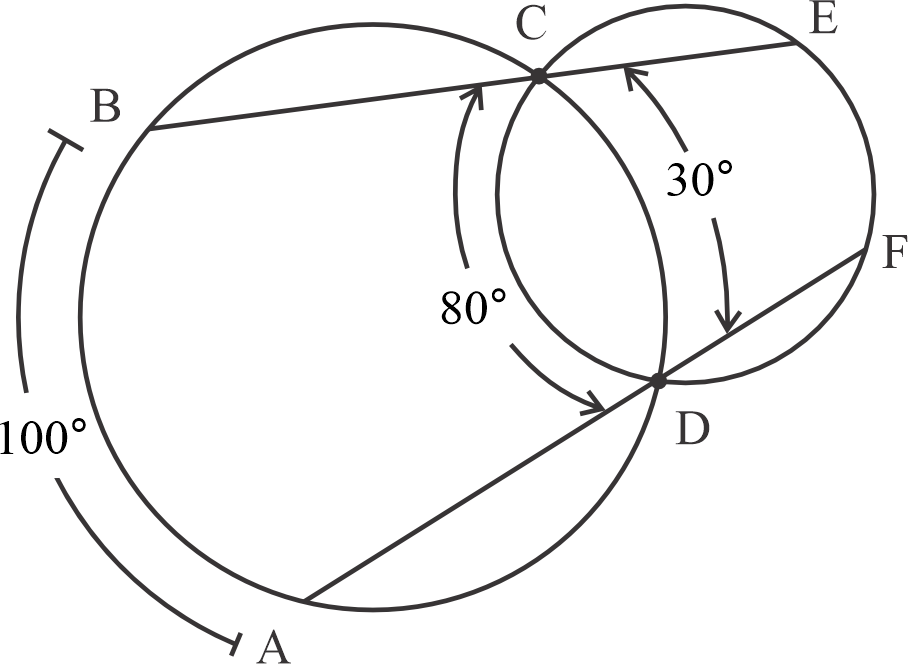
\includegraphics[width=0.3\textwidth]{imagenes/general2024-I/etapa1/bio/geometria1g24-I}
		%\caption{Descripción de la imagen}
		%\label{fig:ejemplo}
	\end{figure}
	
	\begin{enumerate}[label=\alph*)]
		\item $10^\circ$
		\item $20^\circ$
		\item $35^\circ$
		\item $45^\circ$
		\item $50^\circ$
	\end{enumerate}
	
	\textbf{Respuesta correcta:} a)
	
	\vspace{2mm}
	
	\noindent
	\begin{minipage}[t]{0.3\textwidth}
		\vspace{1pt}
		\textbf{Solucionario:}\\[1mm]
		
		De la figura:\\
		
		$\alpha=\dfrac{{100 - 30}}{2} = 35^\circ$\\
		$\alpha  = \dfrac{{80 - x}}{2}$\\
		
		$\to x = 80 - 2\alpha$\\
		$x=80 - 2(35)$\\
		$x = 10^\circ$	
		
	\end{minipage}
	\hfill
	\begin{minipage}[t]{0.7\textwidth}
		\vspace{0pt}
		\centering
		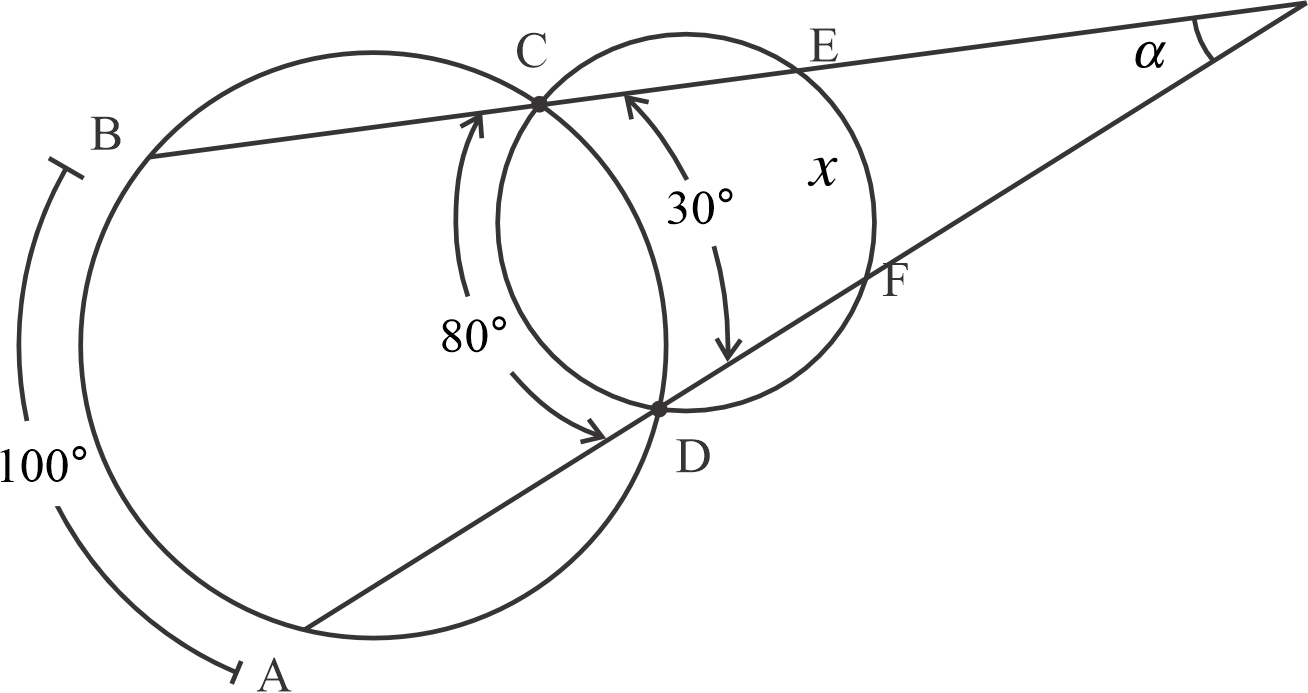
\includegraphics[width=0.7\textwidth]{imagenes/general2024-I/etapa1/bio/geometria1soluciong24-I}
	\end{minipage}
	
	
	
	
	
	
\end{enumerate}



\begin{enumerate}[resume]
	
	\item En la figura	PUNO y UNAP son cuadrados. Si $\alpha=16^\circ$, calcule $x$.
	
	
	\begin{figure}[h]
		\centering
		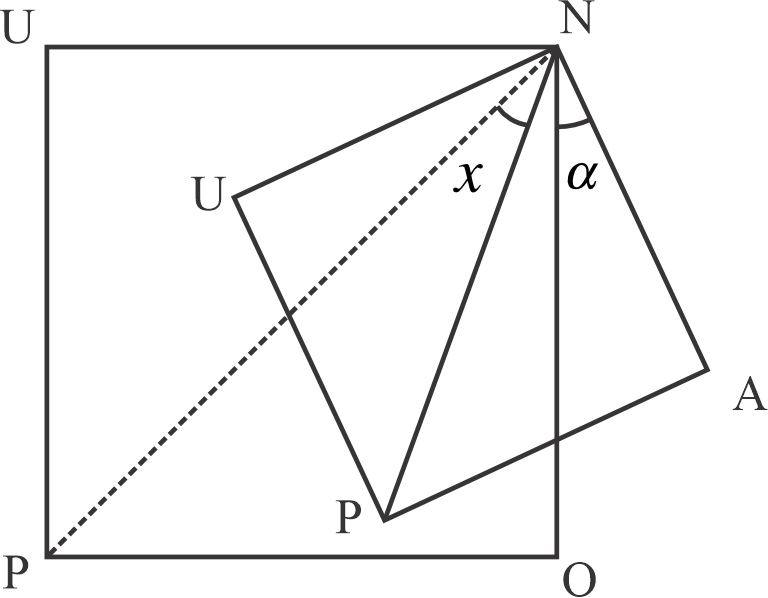
\includegraphics[width=0.37\textwidth]{imagenes/general2024-I/etapa1/bio/geometria2g24-I}
		%\caption{Descripción de la imagen}
		%\label{fig:ejemplo}
	\end{figure}
	
	
	\begin{enumerate}[label=\alph*)]
		\item $15^\circ$
		\item $16^\circ$
		\item $22^\circ$
		\item $31^\circ$
		\item $35^\circ$
	\end{enumerate}
	
	
	\vspace{2mm}
	\textbf{Respuesta correcta:} b)
	
	\vspace{2mm}
	
	
	
	\noindent
	\begin{minipage}[t]{0.3\textwidth}
		\vspace{2pt}
		\textbf{Solucionario:}\\[1mm]
		
		De la figura:\\\\
		${45^\circ } - x + \alpha  = {45^\circ }\\
		x = \alpha \\
		x = 16^\circ$	
		
	\end{minipage}
	\hfill
	\begin{minipage}[t]{0.7\textwidth}
		\vspace{0pt}
		\centering
		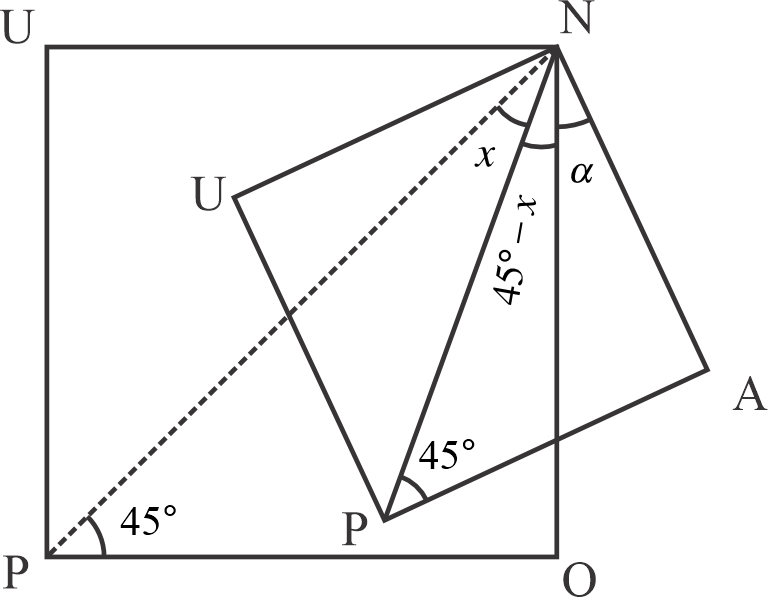
\includegraphics[width=0.55\textwidth]{imagenes/general2024-I/etapa1/bio/geometria2soluciong24-I}
	\end{minipage}
	
	
\end{enumerate}


\begin{enumerate}[resume]
	
	\item Determine la ecuación de la recta que contiene al diamétro de la circunferencia $x^2+y^2-4x-6y=17$ que es perpendicular a la recta $L:5x-2y=13$.
	\begin{enumerate}[label=\alph*)]
		\item $2x+5y-19=0$
		\item $5x+2y-19=0$
		\item $2x-5y-19=0$
		\item $2x+5y+11=0$
		\item $5x+2y+11=0$
	\end{enumerate}
	
	\textbf{Respuesta correcta:} a)
	
	\vspace{2mm}
	\textbf{Solucionario:}\\[1mm]
	
	$x^2+y^2-4x-6y=17\\
	{x-2}^2+{y-3}^2=17+4+9\\
	{x-2}^2+{y-3}^2=30\\
	c=(2,3)\\$
	
	$L:2y =  - 13 + 5x$
	
	$\,\,\,\,\,\,\,\,\,y =  + \dfrac{5}{2}x - \dfrac{{13}}{2} \to {m_1} =  + \dfrac{5}{2}\\$
	
	
	${L_p}:y - {y_0} =  - \dfrac{2}{5}(x - {x_0})$
	
	$\,\,\,\,\,\,\,\,\,5y + 2x + b = 0$
	
	$\,\,\,\,\,\,\,\,5(3) + 2(2) + b = 0$
	
	$\,\,\,\,\,\,\,\,b =  - 19\\$
	
	$\therefore {L_{perpendicular}} : 2x + 5y - 19 = 0$
	
	
	
	
\end{enumerate}


\subsection*{Trigonometría}

\begin{enumerate}[resume]
	
	\item En el gráfico, calcule el área de la región sombreada. 
	
	\begin{figure}[h]
		\centering
		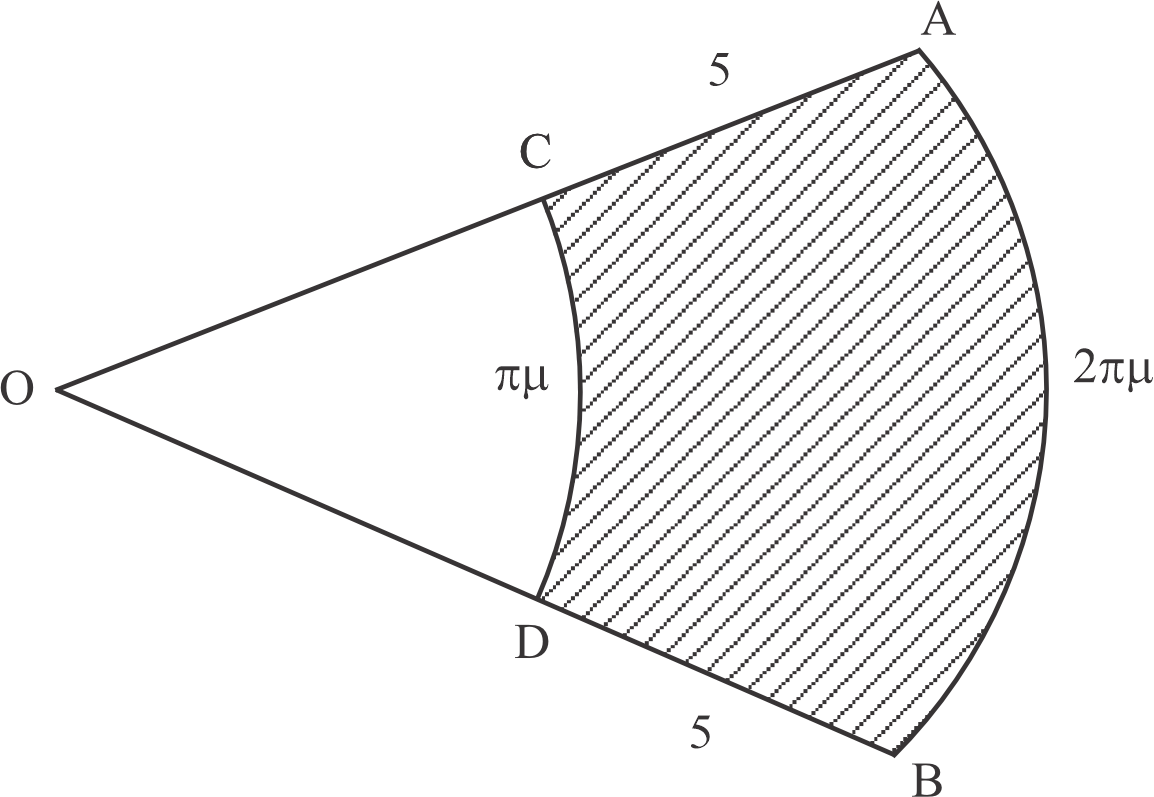
\includegraphics[width=0.48\textwidth]{imagenes/general2024-I/etapa1/bio/trigonometria1g24-I}
		%\caption{Descripción de la imagen}
		%\label{fig:ejemplo}
	\end{figure}
	
	\begin{enumerate}[label=\alph*)]
		\item $\dfrac{{5\pi }}{2}{\mu ^2}$
		\item $\dfrac{{13\pi }}{2}{\mu ^2}$
		\item $\dfrac{{9\pi }}{2}{\mu ^2}$
		\item $\dfrac{{15\pi }}{2}{\mu ^2}$
		\item $\dfrac{{11\pi }}{2}{\mu ^2}$
	\end{enumerate}
	
	\textbf{Respuesta correcta:} d)
	
	\vspace{2mm}
	\textbf{Solucionario:}
	
	\noindent
	\begin{minipage}[t]{0.3\textwidth}
		\vspace{2pt}
		De la figura:\\\\
		${A_S} = \left( {\dfrac{{2\pi  + \pi }}{2}} \right)(5)\\\\
		{A_S} = \left( {\dfrac{{3\pi}}{2}} \right)(5)\\\\
		{A_S} = \dfrac{{15\pi }}{2}{\mu ^2}$	
		
	\end{minipage}
	\hfill
	\begin{minipage}[t]{0.7\textwidth}
		\vspace{0pt}
		\centering
		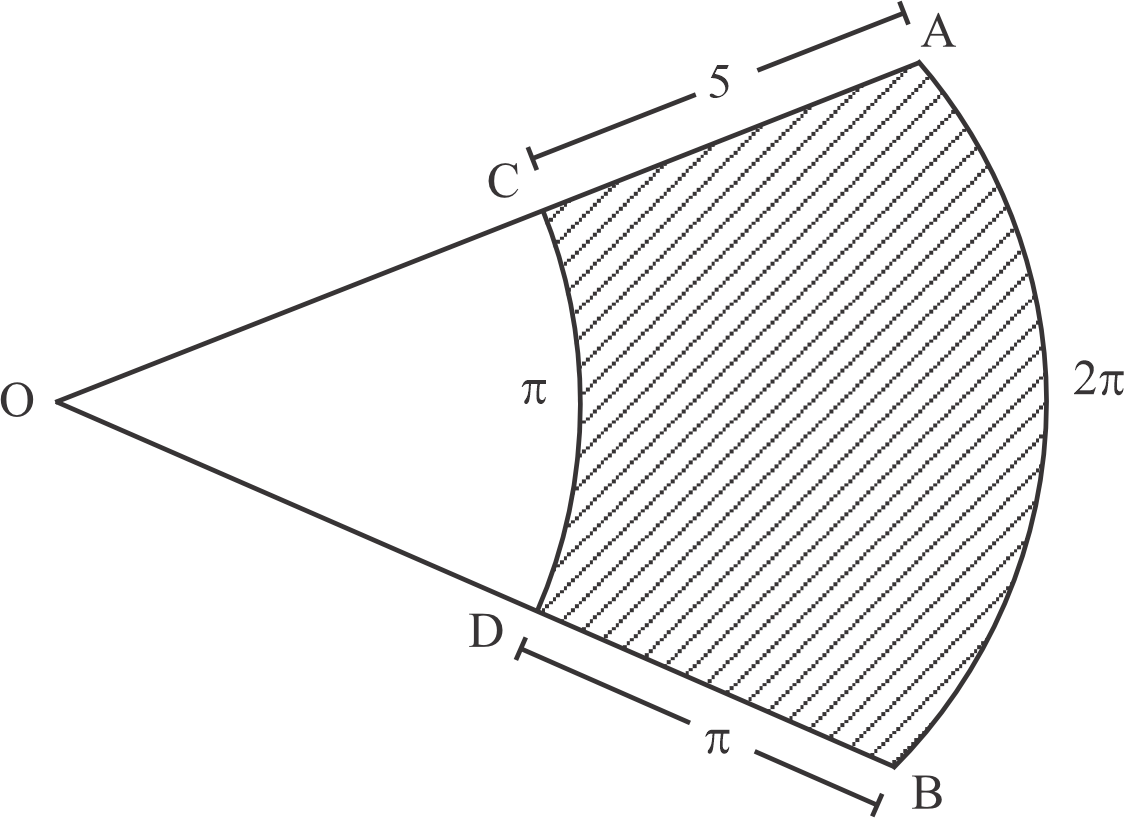
\includegraphics[width=0.65\textwidth]{imagenes/general2024-I/etapa1/bio/trigonometria1soluciong24-I}
	\end{minipage}
	
	
	
\end{enumerate}



\begin{enumerate}[resume]
	
	\item Si A y B son ángulos suplementarios, calcule:
	\[M=cos^2A+sen^2B\]
	\begin{enumerate}[label=\alph*)]
		\item $\,\,\,\,0$
		\item $\,\,\,\,\dfrac{1}{2}$
		\item $\,\,\,\,1$
		\item $-1$
		\item $-\dfrac{1}{2}$
	\end{enumerate}
	
	\textbf{Respuesta correcta:} c)
	
	\vspace{2mm}
	\textbf{Solucionario:}
	
	$A+B=180^\circ\\
	B=180^\circ-A$
	
	$M=cos^2A+sen^2B\\
	M=cos^2A+sen^2(180^\circ-A)\\
	M=cos^2A+(-senA)^2\\
	M=cos^2A+sen^2A\\
	M=1$
	
\end{enumerate}




\begin{enumerate}[resume]
	
	\item En el gráfico, AB$=6$; BC$=5$ y AC$=4$
	
	
	\begin{figure}[h]
		\centering
		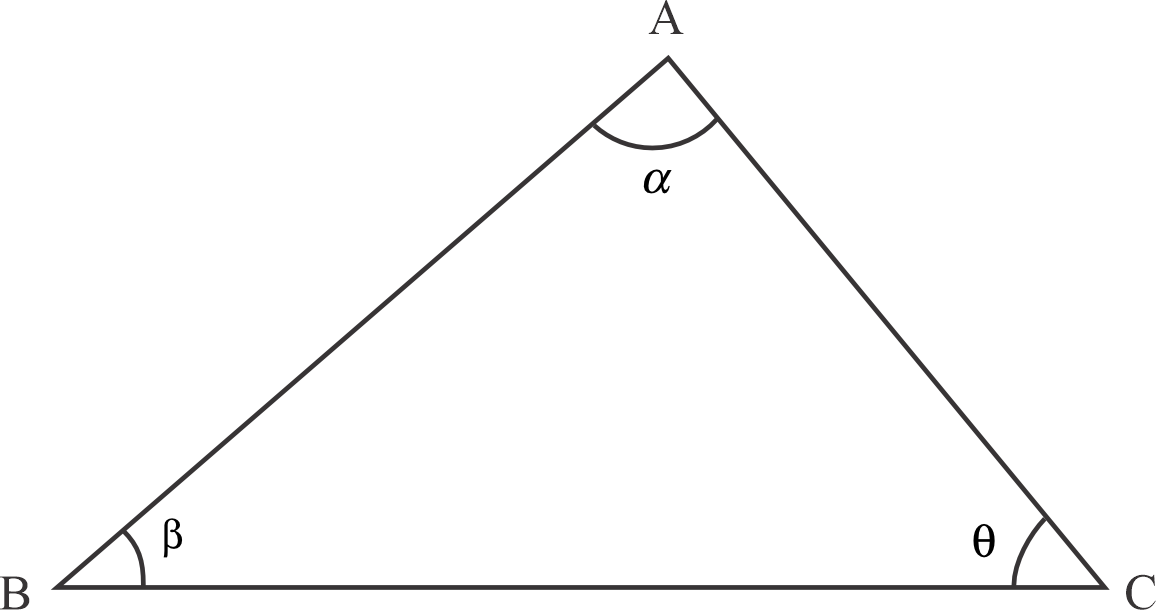
\includegraphics[width=0.5\textwidth]{imagenes/general2024-I/etapa1/bio/trigonometria3g24-I}
		%\caption{Descripción de la imagen}
		%\label{fig:ejemplo}
	\end{figure}
	
	
	Calcule:
	\[M = \dfrac{{sen\alpha  + sen\beta }}{{sen\theta }}\]
	
	\begin{enumerate}[label=\alph*)]
		\item $\dfrac{4}{3}$
		\item $\dfrac{3}{2}$
		\item $\dfrac{3}{4}$
		\item $\dfrac{2}{3}$
		\item $\dfrac{2}{5}$
	\end{enumerate}
	
	\textbf{Respuesta correcta:} b)
	
	\vspace{2mm}
	\textbf{Solucionario:}\\[1mm]
	
	\noindent
	\begin{minipage}[t]{0.35\textwidth}
		\vspace{2pt}
		Ley de senos:\\
		
		$M = \dfrac{{4}}{{sen\beta }}+\dfrac{{5}}{{sen\alpha }}+\dfrac{{6}}{{sen\theta }}=2R\\\\
		M=\dfrac{{sen\beta}}{{4}}+\dfrac{{sen\alpha}}{{5}}+\dfrac{{sen\theta}}{{6}}=\dfrac{{1}}{{2R}}$
		
		$ \left\{ {\begin{array}{*{20}{c}}
				sen\beta=\dfrac{{4}}{{2R}}\\\\
				sen\alpha=\dfrac{{5}}{{2R}}\\\\
				sen\theta=\dfrac{{6}}{{2R}}
		\end{array}} \right.$
		
		$M = \dfrac{{\dfrac{5}{{2R}} + \dfrac{4}{{2R}}}}{{\dfrac{6}{{2R}}}} = \dfrac{{\dfrac{9}{{2R}}}}{{\dfrac{6}{{2R}}}} = \dfrac{9}{6} = \dfrac{3}{2}$	
		
	\end{minipage}
	\hfill
	\begin{minipage}[t]{0.65\textwidth}
		\vspace{0pt}
		\centering
		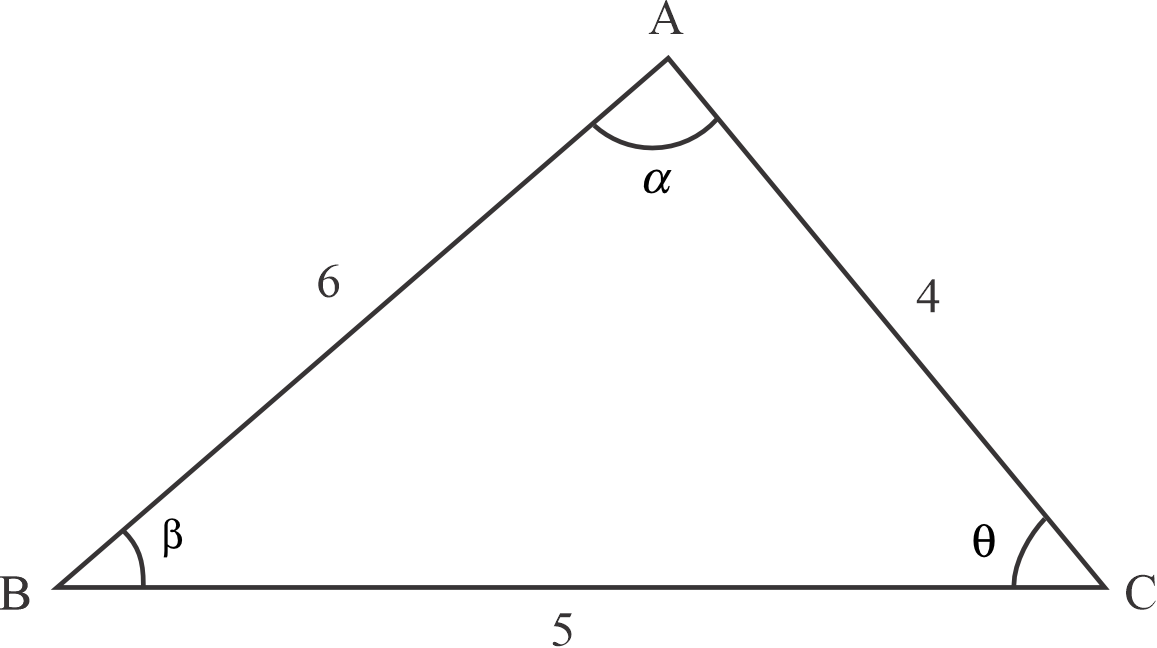
\includegraphics[width=0.8\textwidth]{imagenes/general2024-I/etapa1/bio/trigonometria3soluciong24-I}
	\end{minipage}
	
	
	
	
\end{enumerate}



\subsection*{Física}

\begin{enumerate}[resume]
	
	\item La figura muestra un cubo de arista $x$. Determine módulo de la resultante de los vectores  $\vec{R_1}$ y $\vec{R_2}$.
	
	
	\begin{figure}[h]
		\centering
		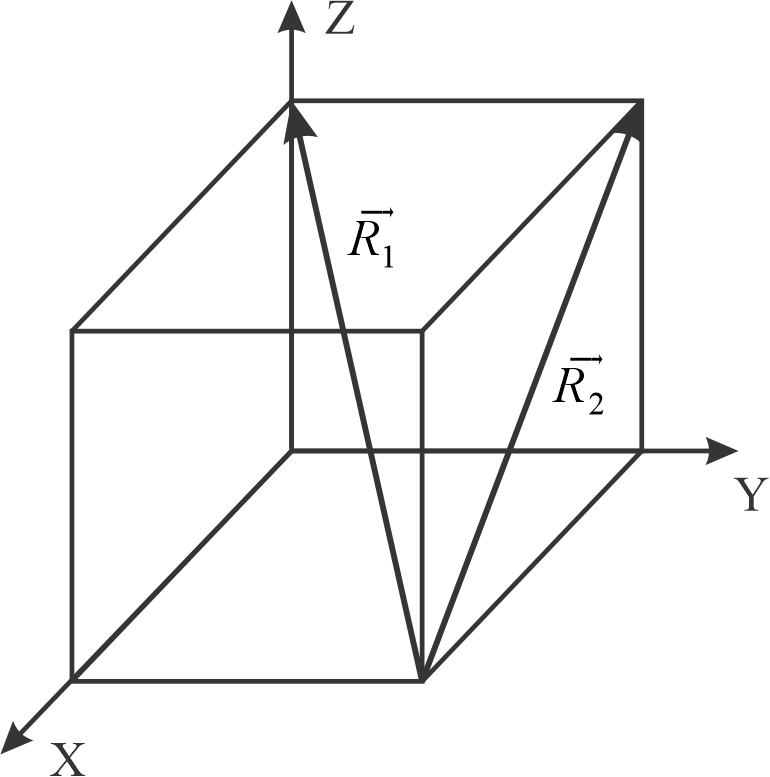
\includegraphics[width=0.3\textwidth]{imagenes/general2024-I/etapa1/bio/fisica1g24-I}
		%\caption{Descripción de la imagen}
		%\label{fig:ejemplo}
	\end{figure}
	
	
	
	\begin{enumerate}[label=\alph*)]
		\item $4x$
		\item $\,\,\,x$
		\item $2x$
		\item $3x$
		\item $5x$
	\end{enumerate}
	
	
	
	
	%\begin{tikzpicture}[overlay, remember picture]
	%	\node at (11, 3) %{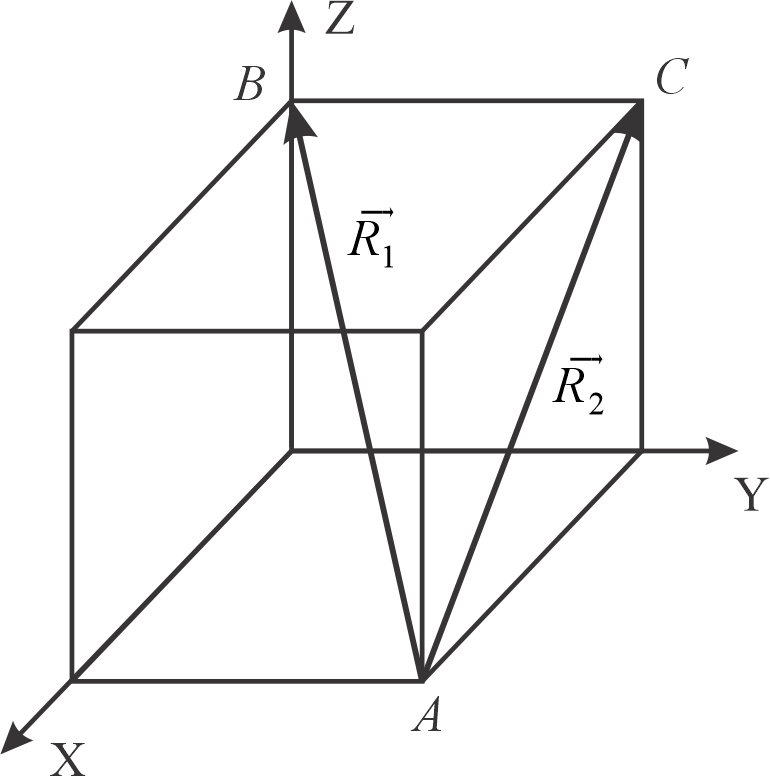
\includegraphics[width=0.4\textwidth]{BIO_PREG1_FISICA_SOLUCION}};
	%\end{tikzpicture}
	
	
	\textbf{Respuesta correcta:} d)
	
	\vspace{2mm}
	\textbf{Solucionario:}\\[1mm]
	
	
	
	
	%\AddToShipoutPicture*{\put(100,80){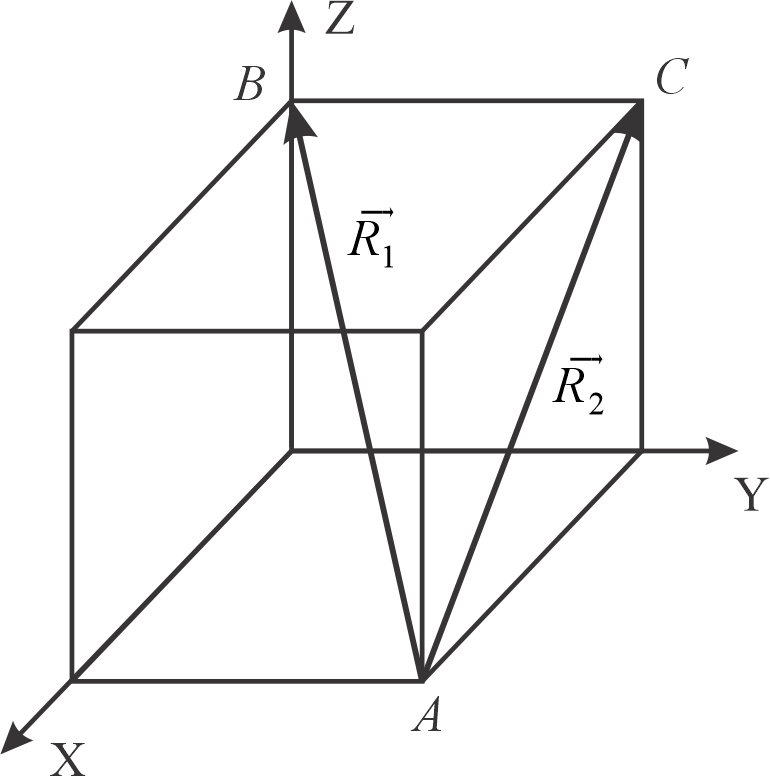
\includegraphics[scale=0.8]{BIO_PREG1_FISICA_SOLUCION}}} % Image background
	
	
	%\begin{figure}[h]
	%	\centering
	%	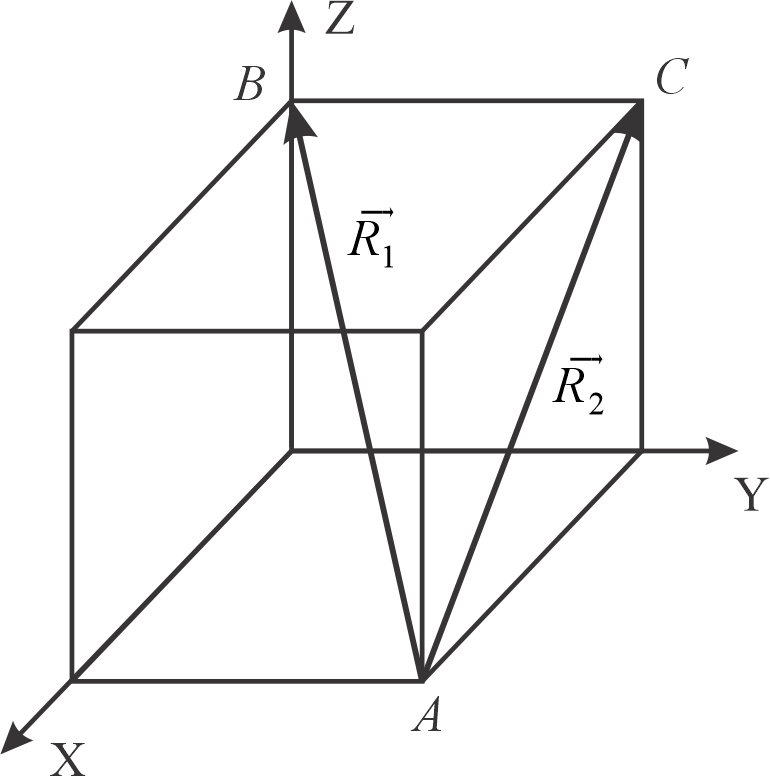
\includegraphics[width=0.4\textwidth]{BIO_PREG1_FISICA_SOLUCION}
	%\AddToShipoutPicture*{\put(100,80){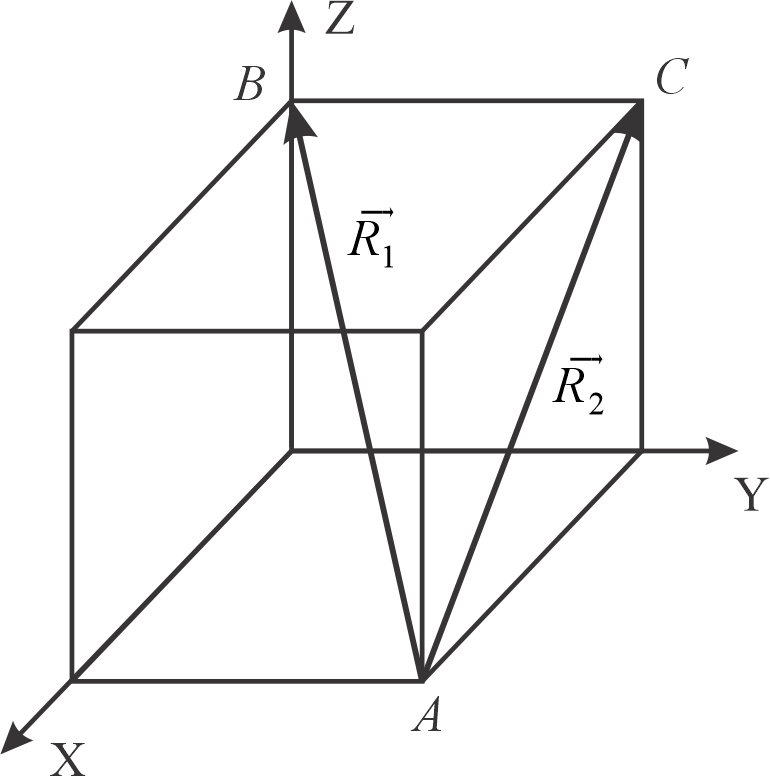
\includegraphics[scale=0.8]{BIO_PREG1_FISICA_SOLUCION}}} % Image background
	%\caption{Descripción de la imagen}
	%\label{fig:ejemplo}
	%\end{figure}
	
	
	De la figura:
	
	$A = (x,x,0)\\
	B = (0,0,x)\\
	C = (0,x,x)$\\
	
	
	$\overrightarrow {{R_{1}}}  = \overrightarrow {AB}  = B - A = (0,0,x) - (x,x,0)\\
	\overrightarrow {{R_{1}}}  = ( - x, - x,x)$
	
	\noindent
	\begin{minipage}[t]{0.5\textwidth}
		\vspace{2pt}
		$\overrightarrow {{R_{2}}}  = \overrightarrow {AC}  = C - A = (0,x,x) - (x,x,0)\\
		\overrightarrow {{R_{2}}}  = ( - x,0,x)\\
		\\$
		
		$\overrightarrow R  = \overrightarrow {{R_{1}}}  + \overrightarrow {{R_{2}}} \\
		\overrightarrow R  = ( - x, - x,x) + ( - x,0,x)\\
		\overrightarrow R  = ( - 2x, - x,2x)$
		
		$\left| {\overrightarrow R } \right| = \sqrt {{{( - 2x)}^2} + {{( - x)}^2} + {{(2x)}^2}}\\\\
		\left| {\overrightarrow R } \right| = \sqrt {{{4x}^2} + {{x}^2} + {{4x}^2}}\\
		\left| {\overrightarrow R } \right| = \sqrt {{{9x}^2}}=3x$	
		
	\end{minipage}
	\hfill
	\begin{minipage}[t]{0.5\textwidth}
		\vspace{0pt}
		\centering
		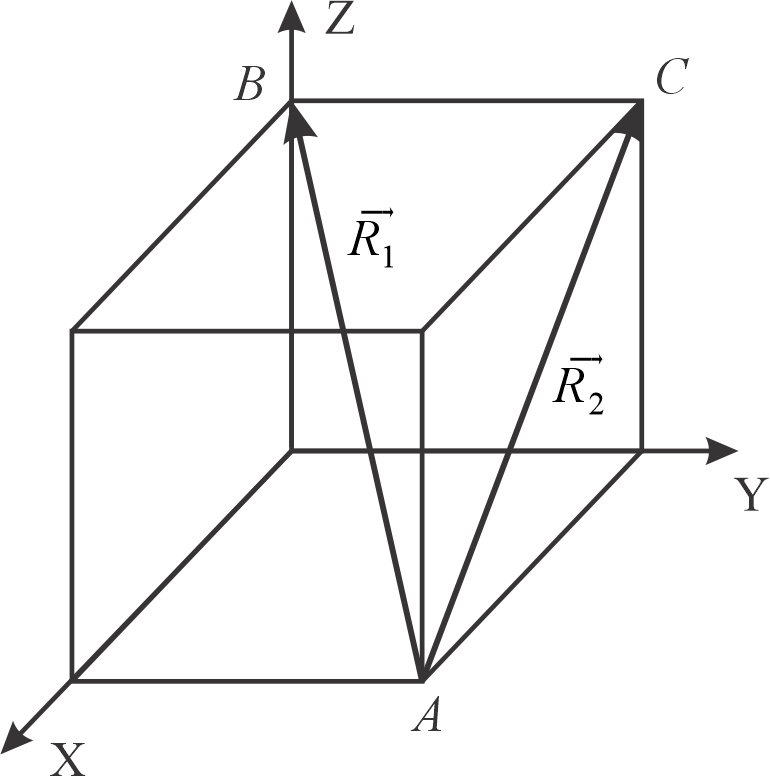
\includegraphics[width=0.68\textwidth]{imagenes/general2024-I/etapa1/bio/fisica1soluciong24-I}
	\end{minipage}
	
	
\end{enumerate}




\begin{enumerate}[resume]
	
	\item Un cuerpo esférico se lanza contra la pared, como se muestra en la figura. Si luego del impacto su rapidez disminuye en $1/3$, determine la relación entre la energía cinética antes y después del impacto. 
	
	
	\begin{figure}[h]
		\centering
		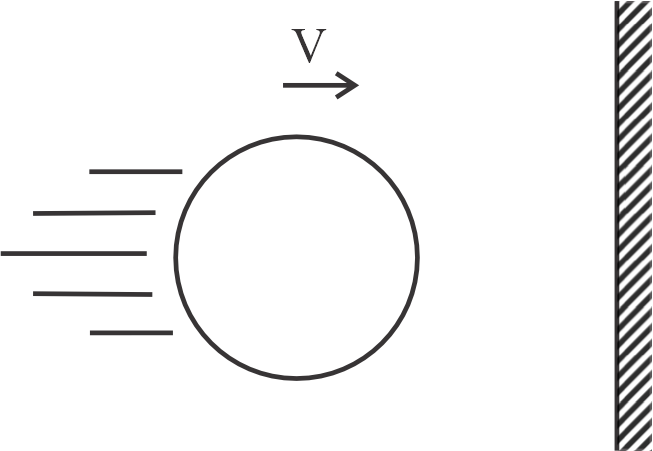
\includegraphics[width=0.3\textwidth]{imagenes/general2024-I/etapa1/bio/fisica2g24-I}
		%\caption{Descripción de la imagen}
		%\label{fig:ejemplo}
	\end{figure}
	
	
	
	\begin{enumerate}[label=\alph*)]
		\item $9/2$
		\item $9/4$
		\item $9/5$
		\item $\,\,\,\,\,9$
		\item $\,\,\,\,\,4$
	\end{enumerate}
	
	\textbf{Respuesta correcta:} b)
	
	\vspace{2mm}
	\textbf{Solucionario:}\\[1mm]
	
	
	$E_{c}\,\text{antes}=\dfrac{1}{2}mv^2\\$
	
	$E_{c}\,\text{después}=\dfrac{1}{2}m({{\dfrac{3}{3}v-\dfrac{1}{3}v}})^2\\\\$
	$E_{c}\,\text{después}=\dfrac{1}{2}m({\dfrac{2}{3}v})^2\\\\$
	$E_{c}\,\text{después}=\dfrac{1}{2}m{\dfrac{4}{2}v}^2=\dfrac{2}{9}mv^2\\$
	
	$\dfrac{{{E_c}\,\text{antes}}}{{{E_c}\,\text{después}}} = \dfrac{{\dfrac{1}{2}m{v^2}}}{{\dfrac{2}{9}m{v^2}}} = \dfrac{9}{4}$
	
	
\end{enumerate}



\begin{enumerate}[resume]
	
	\item Se tiene un alambre largo y delgado por el cual fluye una corriente de $20$ A. ¿A qué distancia del conductor la magnitud del campo magnético es $5\times10^{-4}T$? 
	\newline
	$\mu_o=4\pi\times10^{-7}\,\dfrac{Tm}{\text{A}}$  
	
	
	\begin{enumerate}[label=\alph*)]
		\item $0,4$ cm
		\item $0,5$ cm
		\item $0,6$ cm
		\item $0,7$ cm
		\item $0,8$ cm
	\end{enumerate}
	
	\textbf{Respuesta correcta:} e)
	
	\vspace{2mm}
	
	\noindent
	\begin{minipage}[t]{0.3\textwidth}
		\vspace{2pt}
		\textbf{Solucionario:}\\[1mm]
		
		$B = \dfrac{{{\mu_o}i}}{{2\pi x}}\\\\
		x = \dfrac{{{\mu_o}i}}{{2\pi B}}\\\\
		x = \dfrac{{4\pi  \times {{10}^{ - 7}}\dfrac{{Tm}}{A}(20A)}}{{2\pi (5\times {{10}^{ - 4}}T)}}\\
		x = \dfrac{{4\times {{10}^{ - 6}}}}{{5\times{{10}^{ - 4}}}} = \dfrac{4}{5}\times{10^{ - 2}}m\\\\
		x = 0,8\,cm$
		
	\end{minipage}
	\hfill
	\begin{minipage}[t]{0.7\textwidth}
		\vspace{0pt}
		\centering
		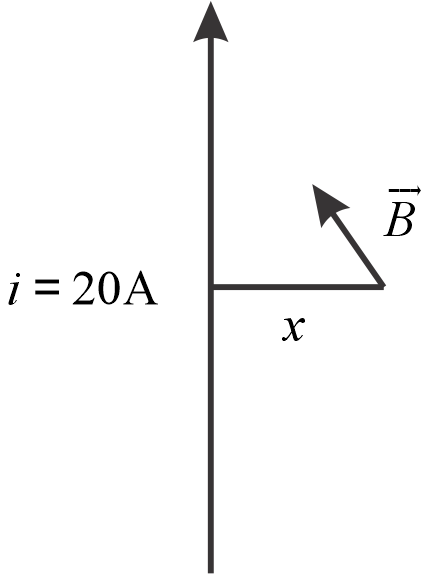
\includegraphics[width=0.3\textwidth]{imagenes/general2024-I/etapa1/bio/fisica3soluciong24-I}
	\end{minipage}
	
	
\end{enumerate}



\subsection*{Química}

\begin{enumerate}[resume]
	
	\item ¿Cuál es la normalidad de una solución que contiene $50$g de ácido sulfúrico en $500$mL de solución?
	\newline
	$(\text{H}=1;\,\text{S}=32;\,\text{O}=16)$
	
	\begin{enumerate}[label=\alph*)]
		\item $2,00$
		\item $2,08$
		\item $2,04$
		\item $2,40$
		\item $2,50$
	\end{enumerate}
	
	\textbf{Respuesta correcta:} c)
	
	\vspace{2mm}
	\textbf{Solucionario:}\\[1mm]
	
	Datos: (H$_2$SO$_4$)
	
	$\text{H}=1\times2\,\,\,=2\\
	\text{S}\,=32\times1=32\\
	\text{O}=16\times4=64$
	
	$\,\,\,\,\,\,\,\,\,\,\,\,\,\,\,\,\,\,\,\,\,\,\,\,\,\,\,\,\,\,=\overline {{\rm{98 g/mol}}}\\$
	
	Volumen solución $=500\text{ml}=0.5\text{L}\\$
	Gramos de soluto $=50\text{g}$\\
	
	Hallando el número equivalente gramo de un ácido:
	
	${\rm{Eq}} - {\rm{g}} = \dfrac{{{\rm{gr}}\,{\rm{soluto}}}}{{{\rm{\# }}\,{\rm{Equivalente}}\,{\rm{gramo}}\,{\rm{\text{ácido}}}\,{\rm{(H)}}}}\\\\
	{\rm{Eq}} - {\rm{g}}\,\,{\rm{\text{ácido}}}\, = \dfrac{{{\rm{gr}}\,{\rm{soluto}}}}{{{\rm{\# }}\,{\rm{Equivalente}}\,{\rm{gramo}}\,{\rm{\text{ácido}}}\,{\rm{(H)}}}}\\\\
	{\rm{Eq}} - {\rm{g}}\,\,{\rm{\text{ácido}}}\,{\rm{\text{sulfúrico}}} = \,49\,{\rm{g}}$\\
	
	Hallando el número equivalente:\\
	${\rm{Eq}} - {\rm{g}} = \dfrac{{50\,{\rm{g}}}}{{49\,{\rm{g}}}} = 1,02\,{\rm{g}}$
	
	Hallando la normalidad:\\
	
	${\rm{N = }}\dfrac{{{\rm{N^\circ  Eq}} - {\rm{g}}}}{{{\rm{U}}\,{\rm{\text{solución}}}}}\\\\
	{\rm{N = }}\dfrac{{1,02}}{{{\rm{0,5}}}}\\\\
	{\rm{N = 2,04}}$
	
	
	
\end{enumerate}


\begin{enumerate}[resume]
	
	\item En la relación a la ecuación química, indique verdadero (V) O (F) según corresponda.
	\[HC{I_{(ac)}} + NaO{H_{(ac)}} \to {H_2}{O_{(l)}} + calor\]
	
	\begin{enumerate}[label=\Roman*.]
		\item Es una reacción de metátesis.
		\item Es una reacción exotérmica.
		\item Es una reacción de simple desplazamiento.
	\end{enumerate}
	
	
	\begin{enumerate}[label=\alph*)]
		\item VVV
		\item FVF
		\item FVV
		\item VVF
		\item FFV
	\end{enumerate}
	
	\textbf{Respuesta correcta:} d)
	
	\vspace{2mm}
	\textbf{Solucionario:}\\[1mm]
	
	
	\begin{enumerate}[label=\Roman*.]
		\item ${\rm{Verdadero}} \to \text{Posee la forma}\,\,\,\,\,\,\,\,{\rm{AB}} + {\rm{CD}} \to {\rm{AC}} + {\rm{BD}}\\
		{\rm{   }} \Rightarrow {\text{corresponde a una reacción de metátesis. }}$
		
		\item ${\rm{Verdadero}} \to \text{Como la reacción genera calor}\\
		{\rm{   }} \Rightarrow {\text{es una reacción exotérmica. }}$
		
		\item ${\rm{Falso}} \to \text{Al ser una reacción de metátesis se desarrolla doble desplazamiento.}$\\
		
	\end{enumerate}
	
\end{enumerate}


\begin{enumerate}[resume]
	
	\item Se necesitan $200$ calorías para que $500$g de un cuerpo eleve su temperatura desde $20^\circ$C hasta $25^\circ$C. Determine el peso atómico de este cuerpo. 
	\begin{enumerate}[label=\alph*)]
		\item $64,5$
		\item $78,7$
		\item $36,4$
		\item $86,5$
		\item $49,5$
	\end{enumerate}
	
	\textbf{Respuesta correcta:} b)
	
	\vspace{2mm}
	\textbf{Solucionario:}\\[1mm]
	
	Datos:\\
	$d=200\,cal$\\
	$m=500 \rm{g}$\\
	$\bigtriangleup T=25-20=5^\circ C$
	
	Según la ley de Dulong y Petit:\\
	$PA \times CE = 6,3\\
	PA = \dfrac{{6,3}}{{CE}}$\\
	
	$d=m\times CE\times \bigtriangleup T\\\\
	CE = \dfrac{{d}}{{m\times \bigtriangleup T}}\\\\
	CE = \dfrac{{200\,cal}}{{500 \rm{g}\times 20^\circ C}}=\dfrac{2}{25}$\\\\
	
	Reemplazando:\\\\
	$PA = \dfrac{{6,3}}{{2/25}} = \dfrac{{25 \times 6,3}}{2} = 25 \times 3,15\\\\
	\boxed{{\therefore PA = 78,7}}$
	
	
\end{enumerate}


\begin{enumerate}[resume]
	
	\item ¿Qué procesos no están relacionados con la electrólisis?
	
	\begin{enumerate}[label=\Roman*.]
		\item La producción de energía eléctrica
		\item La producción de metales con una fina capa de otro metal
		\item La descarga de la batería en los teléfonos móviles
		\item La síntesis de elementos 
		
	\end{enumerate}
	
	
	\begin{enumerate}[label=\alph*)]
		\item Sólo II
		\item Sólo I
		\item Sólo IV
		\item I y III
		\item IV, II y III
	\end{enumerate}
	
	\textbf{Respuesta correcta:} d)
	
	\vspace{2mm}
	\textbf{Solucionario:}
	
	ELECTROLÍSIS\\
	Es un proceso no espontáneo en el cual, por acción de la energía eléctrica que proviene de una fuente de voltaje, se logra desarrollar reacciones REDOX. Se realiza en un medio acuoso. Por lo tanto la producción de energía eléctrica y la descarga de la batería en los teléfonos móviles, no se realiza en medio acuoso.
	
	
\end{enumerate}


\begin{enumerate}[resume]
	
	\item Un gas está confinado en un cilindro de acero de $10,0$ litros, a un apresión de 5 atmósferas y a $27^\circ$C. Si la temperatura se eleva a  $327^\circ$C. ¿Cuál será la presión del gas (en atm) en el interior del cilindro?
	
	\begin{enumerate}[label=\alph*)]
		\item $\,\,\,1,5$
		\item $10,0$
		\item $\,\,\,7,5$
		\item $12,5$
		\item $15,0$
	\end{enumerate}
	
	\textbf{Respuesta correcta:} b)
	
	\vspace{2mm}
	\textbf{Solucionario:}\\[1mm]
	
	
	%\iffalse
	\begin{minipage}[t]{0.45\textwidth}
		Datos:\\
		$V = 10\,L\\
		{P_{\,1}} = 5\,atm\\
		{T_{\,1}} = 27^\circ \rm{C}\\
		{T_{\,2}} = 327^\circ \rm{C}\\
		{P_{\,2}} = ?$
	\end{minipage}
	\hfill
	\begin{minipage}[t]{0.45\textwidth}
		$\dfrac{{{P_{\,1}}}}{{{T_{\,1}}}} = \dfrac{{{P_{\,2}}}}{{{T_{\,2}}}}\\\\
		{P_{\,2}} = \dfrac{{{T_{\,2}}}}{{{T_{\,1}}}}{P_{\,1}}\\\\
		{P_{\,2}} = \dfrac{{327^\circ \rm{C} + 273}}{{27^\circ \rm{C} + 273}}(5\,atm)\\\\
		{P_{\,2}} = \dfrac{{600}}{{300}}(5\,atm)\\\\
		\boxed{{P_{\,2}} = 10\,atm}$
	\end{minipage}
	%\fi
\end{enumerate}

\subsection*{Biología y Anatomía}

\begin{enumerate}[resume]
	
	\item Este parásito es el agente causal de la oxiurasis, se presenta principalmente en grupos familiares e institucionales (guarderías, jardines y escuelas).
	
	\begin{enumerate}[label=\alph*)]
		\item \textit{Enterobius vermicularis}
		\item \textit{Acaris lumbricoides}
		\item \textit{Entamoeba histolytica}
		\item \textit{Fasciola hepática}
		\item \textit{Echinococcus granulosus}
	\end{enumerate}
	
	\textbf{Respuesta correcta:} a)
	
	\vspace{2mm}
	\textbf{Solucionario:}
	
	La oxiurasis o enterobiasis es una parasitosis intestinal producida por \textit{Enterobius vermicularis}, conocido también como oxiuro. Se transmite con facilidad en grupos familiares y escolares por contacto directo o por objetos contaminados. Por ello, la alternativa correcta es \textit{Enterobius vermicularis}.
	
\end{enumerate}


\begin{enumerate}[resume]
	
	\item ¿Cuál es la anomalía cromosómica en la que los testículos se degeneran lentamente y conducen al crecimiento mamario?
	
	\begin{enumerate}[label=\alph*)]
		\item Síndrome de Edwards
		\item Síndrome de Down
		\item Síndrome de Patau 
		\item Síndrome de Klinefelter
		\item Síndrome de Turner
	\end{enumerate}
	
	\textbf{Respuesta correcta:} d)
	
	\vspace{2mm}
	\textbf{Solucionario:}
	
	El síndrome de Klinefelter se presenta en varones con cariotipo 47,XXY. Entre sus características destacan hipogonadismo, degeneración testicular progresiva y ginecomastia (crecimiento mamario). Por eso, la respuesta correcta es síndrome de Klinefelter.
	
\end{enumerate}

\begin{enumerate}[resume]
	
	\item ¿Qué estructura se encuentra exactamente en donde empieza la uretra membranosa?
	
	\begin{enumerate}[label=\alph*)]
		\item próstata
		\item gládula de Cowper
		\item vesísulas seminales 
		\item glándulas de Leydig
		\item glándulas de Skene
	\end{enumerate}
	
	\textbf{Respuesta correcta:} b)
	
	\vspace{2mm}
	\textbf{Solucionario:}
	
	La uretra membranosa se inicia al salir de la próstata y en esa región se relaciona con las glándulas bulbouretrales o glándulas de Cowper. Estas secretan una sustancia lubricante antes de la eyaculación. Por ello, la alternativa correcta es glándula de Cowper.
	
\end{enumerate}


\begin{enumerate}[resume]
	
	\item Durante la profase I de la meiosis, en uno de los periodos, los cromosomas bivalentes alcanzan su estado máximo de condensación, ocurriendo una reducción en el número de quiasmas. Este proceso corresponde a:
	
	\begin{enumerate}[label=\alph*)]
		\item Paquinema 
		\item Diplonema
		\item Cigonema
		\item Diacinesis
		\item Leptonema
	\end{enumerate}
	
	\textbf{Respuesta correcta:} d)
	
	\vspace{2mm}
	\textbf{Solucionario:}
	
	En la diacinesis, etapa final de la profase I, los cromosomas alcanzan su máxima condensación y los quiasmas disminuyen por terminalización. Esa es la característica descrita en el enunciado. Por lo tanto, la respuesta correcta es diacinesis.
	
\end{enumerate}

\begin{enumerate}[resume]
	
	\item ¿Cuál es la asociación interespecífica en la que una de las especies, debido a su desarrollo y producción de sustancias inhibidoras, impide el crecimiento de la otra especie?
	
	\begin{enumerate}[label=\alph*)]
		\item Protocooperación
		\item Amensalismo
		\item Inquilinismo
		\item Comensalismo
		\item Parasitismo
	\end{enumerate}
	
	\textbf{Respuesta correcta:} b)
	
	\vspace{2mm}
	\textbf{Solucionario:}
	
	El amensalismo es una relación interespecífica donde una especie resulta perjudicada y la otra no obtiene beneficio ni daño. Esto ocurre, por ejemplo, cuando una especie libera sustancias inhibidoras que impiden el crecimiento de otra. Por eso, la respuesta es amensalismo.
	
\end{enumerate}


\begin{enumerate}[resume]
	
	\item ¿Cuáles son las células del sistema inmunitario capaces de detectar cambios en las características de algunas células propias que han sido infectadas por virus o que se han degenerado convirtiéndose en células tumorales?
	
	\begin{enumerate}[label=\alph*)]
		\item Linfocitos supresores.
		\item Linfocitos B.
		\item Linfocitos "Helper".
		\item Linfocitos NK.
		\item Linfocitos polimorfonucleares.
	\end{enumerate}
	
	\textbf{Respuesta correcta:} d)
	
	\vspace{2mm}
	\textbf{Solucionario:}
	
	Los linfocitos NK (Natural Killer) reconocen y destruyen células infectadas por virus y células tumorales sin necesidad de una sensibilización previa específica. Su función principal es la vigilancia inmunológica. Por ello, la respuesta correcta es linfocitos NK.
	
\end{enumerate}

\subsection*{Psicología y Filosofía}

\begin{enumerate}[resume]
	
	\item Juana recuerda una imagen que vió en el parque de diversiones. Esta información preliminar específica del cerebro corresponde a:
	
	\begin{enumerate}[label=\alph*)]
		\item el hipotálamo.
		\item el cerebelo.
		\item el tálamo.
		\item el hemisferio izquierdo.
		\item el hemisferio derecho.
	\end{enumerate}
	
	\textbf{Respuesta correcta:} c)
	
	\vspace{2mm}
	\textbf{Solucionario:}
	
	El tálamo actúa como centro de relevo sensorial, organizando e integrando información que luego será procesada por la corteza cerebral. Por ello, ante una información preliminar relacionada con imágenes, la estructura señalada es el tálamo.
	
\end{enumerate}

\begin{enumerate}[resume]
	
	\item Pedro escoge su carrera no porque sea la que más le agrade, sino porque le va proporcionar mayores satisfacciones económicas. ¿Qué actitud asumió Pedro?
	
	\begin{enumerate}[label=\alph*)]
		\item Pragmática
		\item Religiosa
		\item Moral
		\item Definitoria
		\item Problematizadora
	\end{enumerate}
	
	\textbf{Respuesta correcta:} a)
	
	\vspace{2mm}
	\textbf{Solucionario:}
	
	La actitud pragmática se caracteriza por valorar principalmente la utilidad o conveniencia práctica de una decisión. Pedro elige la carrera por el beneficio económico y no por gusto personal. Por eso, la respuesta correcta es pragmática.
	
\end{enumerate}


\begin{enumerate}[resume]
	
	\item Le encanta la compañía, pero aveces busca la soledad; ama profundamente, aveces se desilusiona, lucha y muestra tenacidad por lo que parece su meta, para después decaer y perder el interés.\\\\
	Estas son características de inndividuos que se hallan en la:
	
	
	\begin{enumerate}[label=\alph*)]
		\item senectud.
		\item juventud.
		\item infancia.
		\item adolescencia.
		\item niñez.
	\end{enumerate}
	
	\textbf{Respuesta correcta:} d)
	
	\vspace{2mm}
	\textbf{Solucionario:}
	
	La adolescencia se caracteriza por cambios emocionales intensos, inestabilidad afectiva, contradicciones conductuales y búsqueda de identidad. Las descripciones del enunciado corresponden a esa etapa del desarrollo. Por lo tanto, la respuesta correcta es adolescencia.
	
\end{enumerate}



\begin{enumerate}[resume]
	
	\item \textit{La tierra gira alrededor del sol.}\\\\
	Este enunciado es aceptado por toda la comunidad de individuos cognoscentes en el planeta corresponde al conocimiento:
	
	
	\begin{enumerate}[label=\alph*)]
		\item objetivo.
		\item universal.
		\item necesario.
		\item fundamentado.
		\item racional.
	\end{enumerate}
	
	\textbf{Respuesta correcta:} b)
	
	\vspace{2mm}
	\textbf{Solucionario:}
	
	Un conocimiento es universal cuando su validez es aceptada por todos o tiene alcance general para todos los sujetos cognoscentes. El enunciado dado es reconocido por la comunidad científica y por la humanidad en general. Por eso, corresponde al conocimiento universal.
	
\end{enumerate}


\subsection*{Geografía}

\begin{enumerate}[resume]
	
	\item En el sistema hidrográfico del Perú, la cuenca endorreica corresponde a la vertiente del:
	
	
	\begin{enumerate}[label=\alph*)]
		\item Atlántico.
		\item Pacífico.
		\item Titicaca.
		\item Amazonas.
		\item Marañon.
	\end{enumerate}
	
	\textbf{Respuesta correcta:} c)
	
	\vspace{2mm}
	\textbf{Solucionario:}
	
	Las cuencas endorreicas son aquellas cuyas aguas no desembocan en el mar, sino en lagos interiores. En el Perú, la vertiente endorreica corresponde al lago Titicaca. Por ello, la respuesta correcta es Titicaca.
	
\end{enumerate}

\begin{enumerate}[resume]
	
	\item Los aspectos fundamentales de la biodiversidad son: la variedad genética, la diversidad de especies y la ...
	
	\begin{enumerate}[label=\alph*)]
		\item diversidad de ecosistemas.
		\item megadiversidad.
		\item ecología y desarrollo sotenible.
		\item diversidad botánica.
		\item diversidad zoológica.
	\end{enumerate}
	
	\textbf{Respuesta correcta:} a)
	
	\vspace{2mm}
	\textbf{Solucionario:}
	
	La biodiversidad comprende tres niveles fundamentales: diversidad genética, diversidad de especies y diversidad de ecosistemas. Esta última considera la variedad de hábitats y comunidades ecológicas. Por eso, la respuesta correcta es diversidad de ecosistemas.
	
\end{enumerate}



\subsection*{Historia}

\begin{enumerate}[resume]
	
	\item Entre 1347 y 1353, se produjo la pandemia más mortífera dela historia, conocida como $\_\_\_\_\_\_\_\_\_$. Los síntomas eran fiebre alta, dolores musculares, tos persistente. gangrena en dedos de las extremidades y aparición de enormes ampollas.
	
	\begin{enumerate}[label=\alph*)]
		\item tifoidea
		\item malaria
		\item peste negra
		\item cólera 
		\item peste amarilla
	\end{enumerate}
	
	\textbf{Respuesta correcta:} c)
	
	\vspace{2mm}
	\textbf{Solucionario:}
	
	La pandemia que asoló Europa entre 1347 y 1353 fue la peste negra, una de las más mortíferas de la historia. Produjo millones de muertes y se asoció a bubones, fiebre alta y gangrena. Por ello, la respuesta correcta es peste negra.
	
\end{enumerate}

\begin{enumerate}[resume]
	
	\item En 1856, el Dr. Cayetano Heredia impulsó la creación de la $\_\_\_\_\_\_\_\_\_\_\_$, como ente encargado del entrenamiento y vigilancia de la profesión médica.
	
	\begin{enumerate}[label=\alph*)]
		\item Facultad de Medicina del Perú
		\item Facultad de Medicina del Lima
		\item Facultad de Medicina del San Marcos
		\item Escuela Médica del Perú
		\item Universidad Mayor de San Marcos
		
	\end{enumerate}
	
	\textbf{Respuesta correcta:} b)
	
	\vspace{2mm}
	\textbf{Solucionario:}
	
	La pregunta alude a la reorganización de la enseñanza médica impulsada por Cayetano Heredia en el siglo XIX. Según la clave marcada, la respuesta correcta es Facultad de Medicina de Lima, institución destinada al entrenamiento y vigilancia de la profesión médica.
	
\end{enumerate}


\subsection*{Educación Cívica}


\begin{enumerate}[resume]
	
	\item El Congreso puede delegar al Poder Ejecutivo la facultad de legislar mediante:
	
	\begin{enumerate}[label=\alph*)]
		\item Decreto de Urgencia
		\item Decreto Supremo
		\item Decreto Legislativo
		\item Decreto Ley
		\item Edicto Municipal
	\end{enumerate}
	
	\textbf{Respuesta correcta:} c)
	
	\vspace{2mm}
	\textbf{Solucionario:}
	
	Cuando el Congreso delega facultades legislativas al Poder Ejecutivo, este emite decretos legislativos. Estos tienen rango de ley y se dictan dentro del marco y plazo establecidos por el Congreso. Por lo tanto, la respuesta correcta es Decreto Legislativo.
	
\end{enumerate}

\begin{enumerate}[resume]
	
	\item En el Perú, la entidad autónoma encragada de supervisar la legalidad de la ejecución del presupuesto del Estado es:
	
	\begin{enumerate}[label=\alph*)]
		\item Contraloría General de la República.
		\item Banco Central de Reserva del Perú.
		\item Superintendencia de Banca y Seguros.
		\item Consejo Nacional de la Magistratura.
		\item Jurado Nacional de Elecciones.
	\end{enumerate}
	
	\textbf{Respuesta correcta:} a)
	
	\vspace{2mm}
	\textbf{Solucionario:}
	
	La Contraloría General de la República es el órgano superior del Sistema Nacional de Control. Su función es supervisar la legalidad de la ejecución del presupuesto público y el uso de los recursos del Estado. Por eso, la respuesta correcta es Contraloría General de la República.
	
\end{enumerate}


\subsection*{Economía}

\begin{enumerate}[resume]
	
	\item El creciente desempleo y subempleo en nuestra economía, durante los últimos años, han originado principalmente:
	
	\begin{enumerate}[label=\alph*)]
		\item una mayor apertura de mercados formales.
		\item el incremento de mercados informales.
		\item mayores niveles de ahorro.
		\item un mayor acceso a los mercados cerrados.
		\item un mayor consumo de las familias.
	\end{enumerate}
	
	\textbf{Respuesta correcta:} b)
	
	\vspace{2mm}
	\textbf{Solucionario:}
	
	Cuando aumentan el desempleo y el subempleo, muchas personas recurren a actividades económicas no reguladas para generar ingresos. Eso produce el crecimiento de la informalidad. Por lo tanto, la respuesta correcta es el incremento de mercados informales.
	
\end{enumerate}

\begin{enumerate}[resume]
	
	\item Según los teóricos neoliberales, el Estado debe participar en la economía en la medida en que exista:
	
	\begin{enumerate}[label=\alph*)]
		\item barreras de mercado.
		\item fallas de mercado.
		\item políticas económicas.
		\item posiciones dominantes de mercado.
		\item económias a escala.
	\end{enumerate}
	
	\textbf{Respuesta correcta:} b)
	
	\vspace{2mm}
	\textbf{Solucionario:}
	
	Desde la perspectiva neoliberal, la intervención del Estado debe ser limitada y justificarse principalmente cuando el mercado no asigna eficientemente los recursos. Estas situaciones se denominan fallas de mercado. Por ello, la respuesta correcta es fallas de mercado.
	
\end{enumerate}



\subsection*{Comunicación}

\begin{enumerate}[resume]
	
	\item Consiste en escribir de manera breve y precisa los puntos más resaltantes de un texto en el proceso de la lectura.
	
	\begin{enumerate}[label=\alph*)]
		\item El resumen
		\item Las notas al margen
		\item El esquema
		\item La síntesis
		\item El sumillado
	\end{enumerate}
	
	\textbf{Respuesta correcta:} b)
	
	\vspace{2mm}
	\textbf{Solucionario:}
	
	Las notas al margen consisten en escribir breves apuntes o ideas clave al costado del texto mientras se lee. Sirven para destacar lo más importante de manera precisa y rápida. Por eso, la respuesta correcta es las notas al margen.
	
\end{enumerate}

\begin{enumerate}[resume]
	
	\item La anemia es la disminución de las células rojas de la sangre.\\
	El propósito comunicativo del texto es:
	
	\begin{enumerate}[label=\alph*)]
		\item convencer.
		\item deleitar.
		\item informar.
		\item instruir.
		\item advertir.
	\end{enumerate}
	
	\textbf{Respuesta correcta:} c)
	
	\vspace{2mm}
	\textbf{Solucionario:}
	
	El enunciado brinda una definición objetiva sobre la anemia. No intenta persuadir ni entretener, sino transmitir un dato. Por lo tanto, el propósito comunicativo es informar.
	
\end{enumerate}

\begin{enumerate}[resume]
	
	\item Pedro al culminar sus estudios en el área de Biomédicas, elaborará un documento para que el emitan su certificado de estudios.\\
	¿Qué documento presentar a la coordinación académica de su escuela profesional?
	
	\begin{enumerate}[label=\alph*)]
		\item Oficio
		\item Memorial
		\item Carta
		\item Informe
		\item Solicitud
	\end{enumerate}
	
	\textbf{Respuesta correcta:} e)
	
	\vspace{2mm}
	\textbf{Solucionario:}
	
	Cuando una persona pide formalmente un documento o trámite ante una institución, debe presentar una solicitud. En este caso, Pedro desea que le emitan su certificado de estudios. Por ello, la respuesta correcta es solicitud.
	
\end{enumerate}


\begin{enumerate}[resume]
	
	\item La función del lenguaje que expresa el mundo interior del sujeto es la:
	
	\begin{enumerate}[label=\alph*)]
		\item poética.
		\item metalinguística.
		\item apelativa.
		\item fática.
		\item expresiva.
	\end{enumerate}
	
	\textbf{Respuesta correcta:} e)
	
	\vspace{2mm}
	\textbf{Solucionario:}
	
	La función expresiva o emotiva del lenguaje manifiesta sentimientos, emociones, estados de ánimo y opiniones del hablante. Como el enunciado se refiere al mundo interior del sujeto, la respuesta correcta es expresiva.
	
\end{enumerate}


\subsection*{Literatura}

\begin{enumerate}[resume]
	
	\item ¿Qué figuras literarias están presentes en los versos?\\\\
	"Si eres muerte, ¿por qué me das la vida?\\ 
	si eres vida, ¿por qué me das la muerte?"
	
	\begin{enumerate}[label=\alph*)]
		\item Epítelo y simil
		\item Anáfora y metáfora
		\item Anáfora y paradoja
		\item Anáfora y antítesis
		\item Metáfora y retruécano
	\end{enumerate}
	
	\textbf{Respuesta correcta:} c)
	
	\vspace{2mm}
	\textbf{Solucionario:}
	
	Hay anáfora porque se repite la estructura inicial ``si eres...''. Además, existe paradoja porque se unen ideas aparentemente contradictorias: muerte que da vida y vida que da muerte. Por eso, la respuesta correcta es anáfora y paradoja.
	
\end{enumerate}

\begin{enumerate}[resume]
	
	\item ¿Cuál es el mensaje que evoca los versos del poema Heraldos Negros?\\\\
	Hay golpes en la vida tan fuertes ... ¡Yo no sé!\\
	golpes como el odio de Dios\\
	como si ante ello,\\
	la resaca de todo lo sufrido\\
	se empozara en el alma ... ¡Yo no sé!
	
	\begin{enumerate}[label=\alph*)]
		\item El poeta expresa en forma dolida el sufrimiento humano.
		\item El poeta expresa el odio al hombre.
		\item El poeta percibe el odio de Dios.
		\item El poeta percibe la incomprensión a las penurias del hombre.
		\item El poeta suspira y se congoja sin causa.
	\end{enumerate}
	
	\textbf{Respuesta correcta:} a)
	
	\vspace{2mm}
	\textbf{Solucionario:}
	
	En los versos de \textit{Los heraldos negros}, César Vallejo expresa el dolor profundo que causan ciertos golpes de la vida. El tema central es el sufrimiento humano ante experiencias dolorosas e inexplicables. Por ello, la respuesta correcta es la alternativa a).
	
\end{enumerate}

\subsection*{Razonamiento Matemático}

\begin{enumerate}[resume]
	
	\item Tres pasajeras se sientan alrededor de una mesa circular con 6 sillas distribuidas simétricamente. Se sabe que:
	
	\begin{itemize}[label=--]
		\item A la derecha de la novia de Alberto se sienta Gabriel.
		\item Mary, que está sentada a la derecha de Dora, está sentada al frente de su propio novio.
		\item Alberto está a la izquierda de Mario.
		\item Esperanza está al frente de la novia de Gabriel.
	\end{itemize}
	
	¿Quién es el novio de Dora?
	
	\begin{enumerate}[label=\alph*)]
		\item Antonio
		\item Gabriel
		\item Alberto
		\item Mario
		\item José
	\end{enumerate}
	
	\textbf{Respuesta correcta:} b)
	
	\vspace{2mm}
	\textbf{Solucionario:}\\
	
	Iniciando con el último dato.
	
	\noindent
	\begin{minipage}[t]{0.40\textwidth}
		\vspace{5pt}
		Del segundo dato, Mary está al frente de su propio novio, por tanto no puede ser Mary.
		
		Tampoco puede ser Esperanza, entonces la única posibilidad es que la novia de Gabriel sea Dora.
		
		$\therefore$ El novio de Dora es Gabriel.
	\end{minipage}
	\hfill
	\begin{minipage}[t]{0.35\textwidth}
		\vspace{0pt}
		\centering
		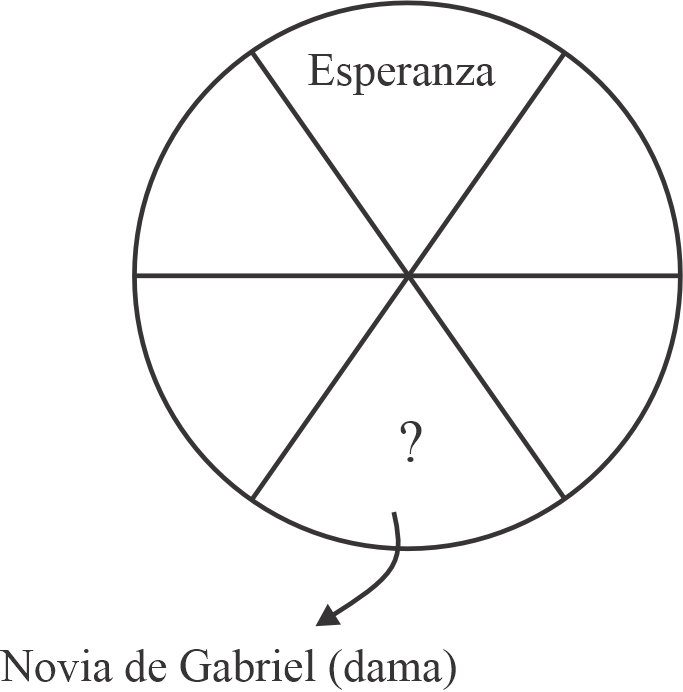
\includegraphics[width=4cm]{imagenes/general2024-I/etapa1/bio/razonamientomatematico1soluciong24-I}
	\end{minipage}
	
\end{enumerate}

\begin{enumerate}[resume]
	
	\item En un concierto hay tantas parejas bailando como varones parados. 300 damas no bailan, si las personas que no bailan son el triple de las damas que bailan, además hay 100 varones más bailando que sentados. ¿Cuántos varones bailan?
	
	\begin{enumerate}[label=\alph*)]
		\item $100$
		\item $150$
		\item $200$
		\item $150$
		\item $300$
	\end{enumerate}
	
	\textbf{Respuesta correcta:} c)
	
	\vspace{2mm}
	\textbf{Solucionario:}\\
	
	\begin{figure}[h]
		\centering
		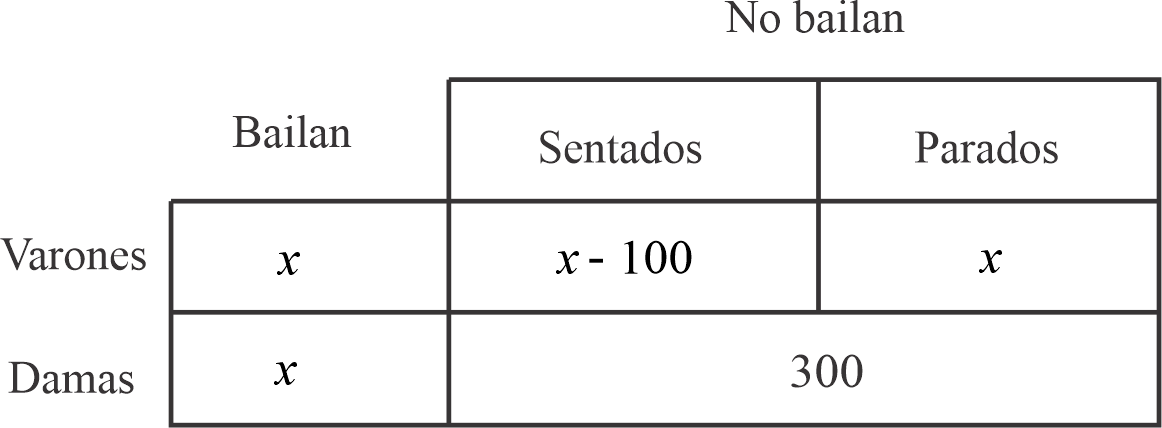
\includegraphics[width=5.5cm]{imagenes/general2024-I/etapa1/bio/razonamientomatematico2soluciong24-I}
	\end{figure}
	
	Planteando sobre las parejas que no bailan:
	
	$x-100+x+300=3x$
	
	$2x+200=3x$
	
	$x=200$
	
	$\therefore$ El número de hombres que bailan es $200$.
	
\end{enumerate}

\begin{enumerate}[resume]
	
	\item Un estudiante universitario multiplica el día de su nacimiento por 12 y el número del mes por 31. Luego suma ambos productos y obtiene 277. Determine la fecha de nacimiento de dicha persona.
	
	\begin{enumerate}[label=\alph*)]
		\item 5 de junio
		\item 7 de junio
		\item 7 de julio
		\item 5 de julio
		\item 12 de julio
	\end{enumerate}
	
	\textbf{Respuesta correcta:} d)
	
	\vspace{2mm}
	\textbf{Solucionario:}\\
	
	Sea la fecha de nacimiento:
	
	$\text{Día} \to D$
	
	$\text{Mes} \to M$
	
	Planteando la ecuación diofántica:
	
	$12D+31M=277$
	
	Probando la alternativa correcta:
	
	$12(5)+31(7)=60+217=277$
	
	$\therefore$ La fecha de nacimiento es 5 de julio.
	
\end{enumerate}

\begin{enumerate}[resume]
	
	\item ¿Cuántos cuadriláteros hay en la sucesión de figuras?
	
	\begin{figure}[h]
		\centering
		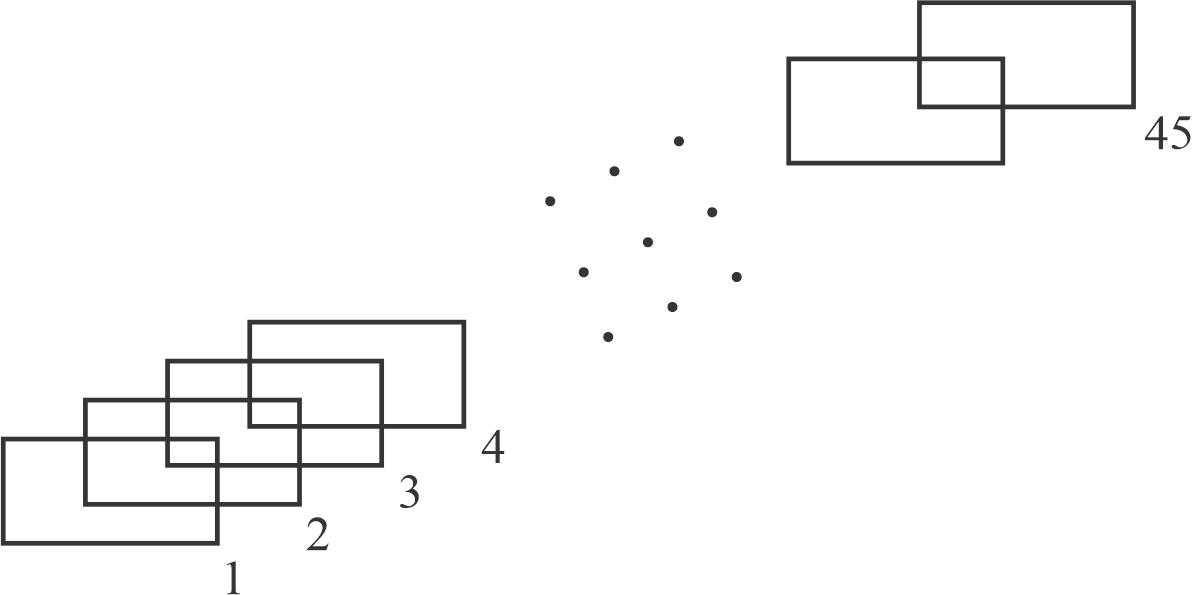
\includegraphics[width=5.5cm]{imagenes/general2024-I/etapa1/bio/razonamientomatematico4g24-I}
	\end{figure}
	
	\begin{enumerate}[label=\alph*)]
		\item 168
		\item 318
		\item 268
		\item 350
		\item 218
	\end{enumerate}
	
	\textbf{Respuesta correcta:} e)
	
	\vspace{2mm}
	\textbf{Solucionario:}\\
	
	Del gráfico se deduce:
	
	\begin{figure}[h]
		\centering
		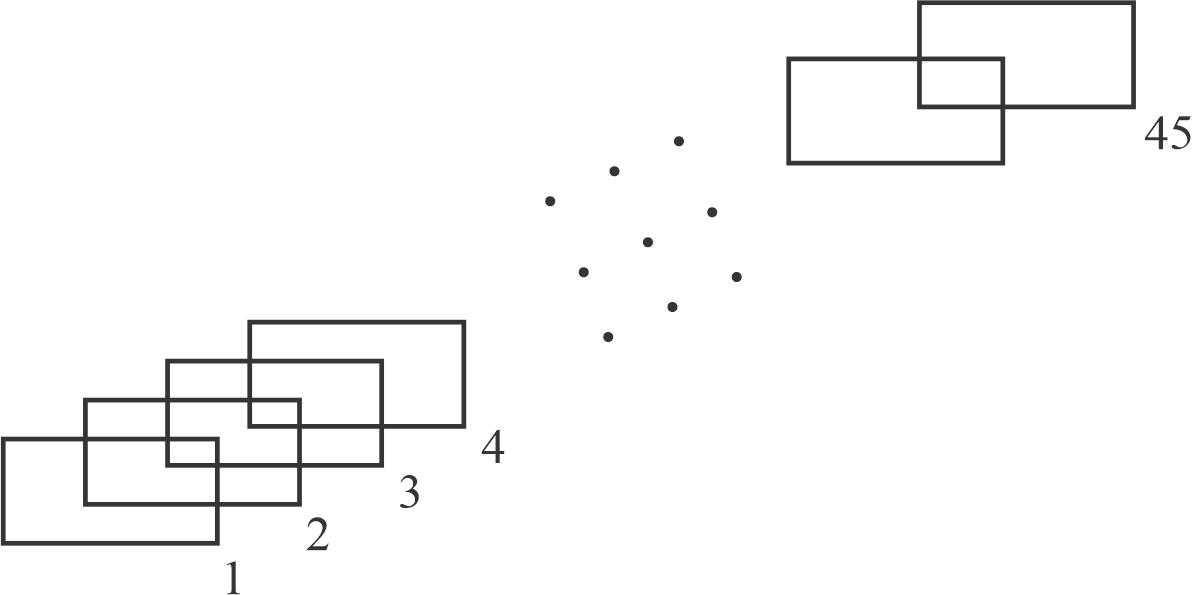
\includegraphics[width=5.5cm]{imagenes/general2024-I/etapa1/bio/razonamientomatematico4g24-I}
	\end{figure}
	
\end{enumerate}

\newpage

\begin{enumerate}[resume]
	
	\item La figura mostrada \textit{ABCD} es un cuadrado, donde \textit{P} y \textit{Q} son puntos medios. ¿Qué porcentaje del área del cuadrado es el área de las regiones sombreadas?
	
	\begin{figure}[h]
		\centering
		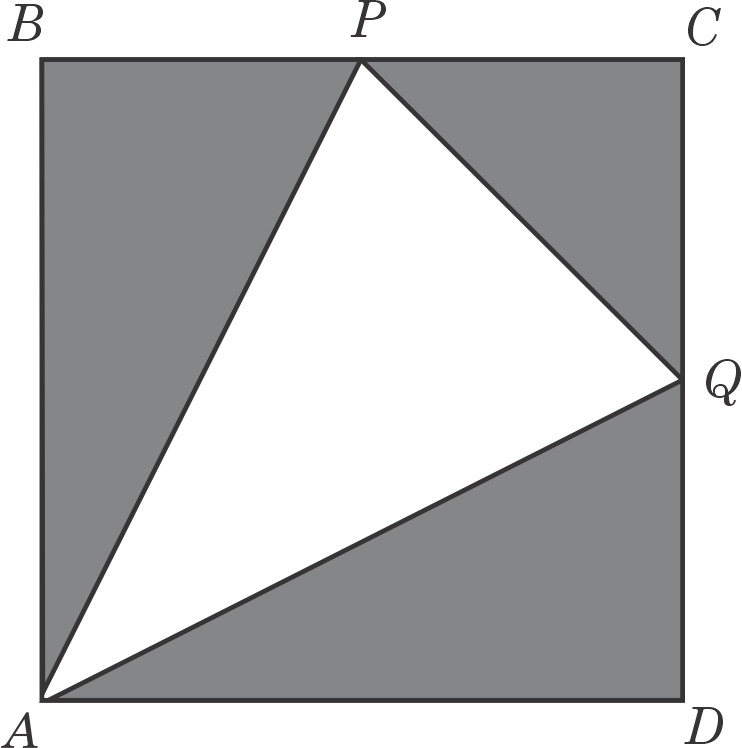
\includegraphics[width=3.5cm]{imagenes/general2024-I/etapa1/bio/razonamientomatematico5g24-I}
	\end{figure}
	
	\begin{enumerate}[label=\alph*)]
		\item $72\%$
		\item $52.5\%$
		\item $75\%$
		\item $62.5\%$
		\item $60\%$
	\end{enumerate}
	
	\textbf{Respuesta correcta:} d)
	
	\vspace{2mm}
	\textbf{Solucionario:}\\
	
	\noindent
	\begin{minipage}[t]{0.40\textwidth}
		\vspace{12pt}
		Según el gráfico:
		
		$50\%+\dfrac{1}{4}50\%$
		
		$50\%+12,5\%=62.5\%$
	\end{minipage}
	\hfill
	\begin{minipage}[t]{0.35\textwidth}
		\vspace{0pt}
		\centering
		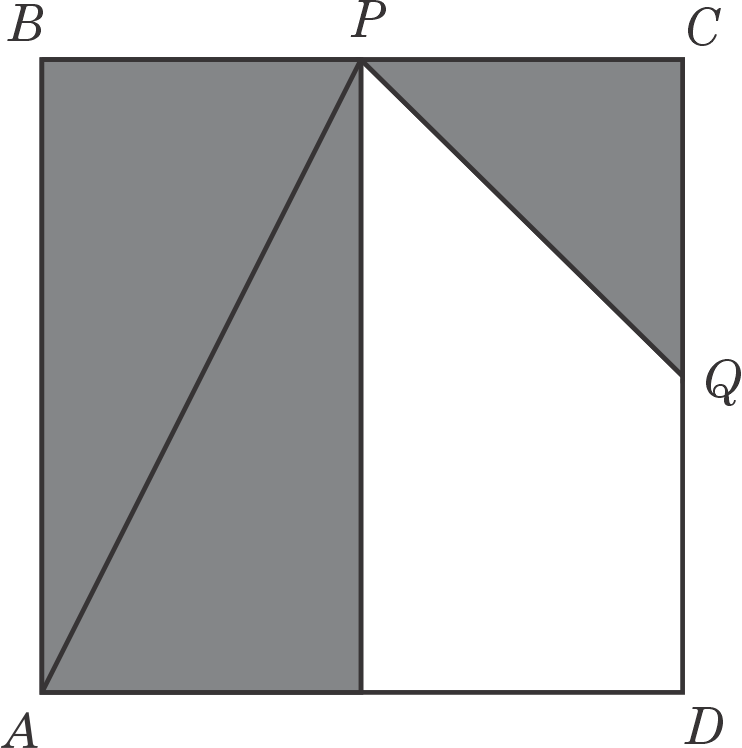
\includegraphics[width=3.5cm]{imagenes/general2024-I/etapa1/bio/razonamientomatematico5soluciong24-I}
	\end{minipage}
	
\end{enumerate}

\begin{enumerate}[resume]
	
	\item Calcule $x$:
	
	$\dfrac{x(x-1)!(x!-21)}{4!}=1+2!$
	
	\begin{enumerate}[label=\alph*)]
		\item 5
		\item 4
		\item 6
		\item 2
		\item 12
	\end{enumerate}
	
	\textbf{Respuesta correcta:} b)
	
	\vspace{2mm}
	\textbf{Solucionario:}\\
	
	$\dfrac{x(x-1)!(x!-21)}{4!}=1+2!$
	
	$\dfrac{x(x-1)!(x!-21)}{24}=1+2$
	
	$x!(x!-21)=72$
	
	$(x!)^2-21x!-72=0$
	
	Entonces:
	
	$(x!-24)(x!+3)=0$
	
	$x!=24 \qquad \text{o} \qquad x!=-3$
	
	Como $x!>0$, se tiene:
	
	$x!=24$
	
	$4!=24$
	
	$\therefore x=4$
	
\end{enumerate}


\subsection*{Razonamiento Verbal}

\begin{enumerate}[resume]
	
	\item Muchos de nuestros políticos son unos demagogos. Etimológicamente la palabra demagogo significa:
	
	\begin{enumerate}[label=\alph*)]
		\item \begin{tabular}{p{2.5cm} cp{3cm}} pueblo & -- & maestro. \end{tabular}
		\item \begin{tabular}{p{2.5cm} cp{3cm}} libertad & -- & ahora. \end{tabular}
		\item \begin{tabular}{p{2.5cm} cp{3cm}} democracia & -- & participativa. \end{tabular}
		\item \begin{tabular}{p{2.5cm} cp{3cm}} pueblo & -- & conductor. \end{tabular}
		\item \begin{tabular}{p{2.5cm} cp{3cm}} niño & -- & conductor. \end{tabular}
	\end{enumerate}
	
	\textbf{Respuesta correcta:} d)
	
	\vspace{2mm}
	\textbf{Solucionario:}\\[1mm]
	La pregunta pide el significado \textbf{etimológico} de la palabra \textit{demagogo}; es decir, su sentido a partir de las raíces griegas que la componen.
	
	La palabra \textit{demagogo} proviene del griego:
	
	\begin{itemize}[label=--]
		\item \textit{demos}: pueblo.
		\item \textit{agogos}: conductor, guía, el que conduce.
	\end{itemize}
	
	Por tanto, etimológicamente, \textit{demagogo} significa literalmente:
	
	\[
	\text{demagogo} = \text{pueblo} + \text{conductor}
	\]
	
	Es decir, \textbf{conductor del pueblo} o \textbf{el que guía al pueblo}.
	
	\vspace{6mm}
	
	\item Complete la oración\\
	A los psicólogos sociales podría considerárseles los médicos de la sociedad ... son los encargados de sanar los males que atacan a grupos humanos; ... ellos solo proporcionan los medios para que cada conglomerado humano saque sus propias conclusiones. 
	
	\begin{enumerate}[label=\alph*)]
		\item \begin{tabular}{p{2.5cm} cp{3cm}} ya que & -- & y \end{tabular}
		\item \begin{tabular}{p{2.5cm} cp{3cm}} pues & -- & por el contrario \end{tabular}
		\item \begin{tabular}{p{2.5cm} cp{3cm}} en tanto & -- & en consecuencia \end{tabular}
		\item \begin{tabular}{p{2.5cm} cp{3cm}} pero & -- & no obstante \end{tabular}
		\item \begin{tabular}{p{2.5cm} cp{3cm}} porque & -- & aunque \end{tabular}
	\end{enumerate}
	
	\textbf{Respuesta correcta:} e)
	
	\vspace{2mm}
	\textbf{Solucionario:}\\[1mm]
	Para resolver este tipo de ejercicios, debemos identificar la \textbf{relación lógica} entre las partes de la oración.
	
	\textit{A los psicólogos sociales podría considerárseles los médicos de la sociedad \textbf{porque} son los encargados de sanar los males que atacan a grupos humanos; \textbf{aunque} ellos solo proporcionan los medios para que cada conglomerado humano saque sus propias conclusiones.}
	
	La oración queda coherente:
	
	\begin{itemize}[label=--]
		\item \textbf{porque} explica la causa;
		\item \textbf{aunque} introduce una precisión restrictiva.
	\end{itemize}
	
	Revisemos por qué las demás no son las mejores:
	
	\begin{itemize}[label=--]
		\item a) \textit{ya que -- y}: el segundo conector solo suma, pero no expresa restricción.
		\item b) \textit{pues -- por el contrario}: el segundo establece oposición muy fuerte, no una concesión.
		\item c) \textit{en tanto -- en consecuencia}: el segundo indica resultado, lo cual no corresponde.
		\item d) \textit{pero -- no obstante}: ambos son adversativos; el primero no expresa adecuadamente la causa.
	\end{itemize}
	
	Por lo tanto, la alternativa correcta es \textbf{e)}.
	
	\vspace{6mm}
	
	\item Resuelve el siguiente par analógico.\\
	ADENITIS : GLÁNDULAS ::
	
	\begin{enumerate}[label=\alph*)]
		\item \begin{tabular}{p{2.5cm} cp{3cm}} cistitis & : & cejas. \end{tabular}
		\item \begin{tabular}{p{2.5cm} cp{3cm}} otitis & : & oídos. \end{tabular}
		\item \begin{tabular}{p{2.5cm} cp{3cm}} meningitis & : & meniscos. \end{tabular}
		\item \begin{tabular}{p{2.5cm} cp{3cm}} poliomelitis & : & huesos. \end{tabular}
		\item \begin{tabular}{p{2.5cm} cp{3cm}} blefaritis & : & labios. \end{tabular}
	\end{enumerate}
	
	\textbf{Respuesta correcta:} b)
	
	\vspace{2mm}
	\textbf{Solucionario:}\\[1mm]
	La relación analógica planteada es:
	
	\[
	\text{nombre de enfermedad o inflamación} : \text{órgano o parte afectada}
	\]
	
	Analicemos el primer par:
	
	\begin{itemize}[label=--]
		\item \textit{Adenitis} = inflamación de las glándulas.
	\end{itemize}
	
	Entonces debemos buscar otra relación semejante:
	
	\[
	\text{inflamación} : \text{órgano afectado}
	\]
	
	Revisemos las opciones:
	
	\begin{itemize}[label=--]
		\item a) \textit{cistitis} : cejas\\
		Cistitis es inflamación de la vejiga, no de las cejas.
		
		\item b) \textit{otitis} : oídos\\
		Otitis es inflamación del oído. La relación es correcta.
		
		\item c) \textit{meningitis} : meniscos\\
		Meningitis es inflamación de las meninges, no de los meniscos.
		
		\item d) \textit{poliomielitis} : huesos\\
		La poliomielitis afecta el sistema nervioso, no los huesos.
		
		\item e) \textit{blefaritis} : labios\\
		Blefaritis es inflamación de los párpados, no de los labios.
	\end{itemize}
	
	La única alternativa que conserva exactamente la misma relación es:
	
	\[
	\text{otitis} : \text{oídos}
	\]
	
	Por ello, la respuesta correcta es \textbf{b)}.
	
	\vspace{6mm}
	
	\item ELIMINACIÓN DE ORACIONES
	
	\begin{enumerate}[label=\alph*)]
		\item El problema surge a partir de la observación.
		\item El conocimiento surge a partir de la investigación.
		\item Una buena investigación implica observación.
		\item Los sentidos deben estar en óptimo nivel para percibir.
		\item La observación debe ser objetiva.
	\end{enumerate}
	
	\textbf{Respuesta correcta:} d)
	
	\vspace{2mm}
	\textbf{Solucionario:}\\[1mm]
	En eliminación de oraciones debemos identificar cuál de los enunciados \textbf{rompe la unidad temática} o se aleja de la idea central.
	
	Observemos el tema común de las oraciones:
	
	\begin{itemize}[label=--]
		\item a) relaciona la observación con el surgimiento del problema.
		\item b) relaciona la investigación con el conocimiento.
		\item c) vincula directamente investigación y observación.
		\item e) señala una característica propia de la observación: la objetividad.
	\end{itemize}
	
	En todas ellas el eje temático es el \textbf{proceso de observación e investigación} como base del conocimiento.
	
	En cambio, la oración:
	
	\textit{Los sentidos deben estar en óptimo nivel para percibir}
	
	se enfoca en una condición biológica o fisiológica de la percepción sensorial, no en la observación como método de investigación ni en su valor epistemológico.
	
	Es decir:
	
	\begin{itemize}[label=--]
		\item no desarrolla directamente la idea de investigación;
		\item no explica la objetividad de la observación;
		\item no se integra con precisión al conjunto.
	\end{itemize}
	
	Por eso, la oración que se debe eliminar es la \textbf{d)}.
	
	\vspace{6mm}
	
	\item El sinónimo de la palabra MEFÍTICO es:
	
	\begin{enumerate}[label=\alph*)]
		\item inodoro.
		\item corrosivo.
		\item insípido.
		\item irrespirable.
		\item expansivo.
	\end{enumerate}
	
	\textbf{Respuesta correcta:} d)
	
	\vspace{2mm}
	\textbf{Solucionario:}\\[1mm]
	La palabra \textit{mefítico} se usa para describir algo que:
	
	\begin{itemize}[label=--]
		\item despide emanaciones fétidas o nocivas;
		\item tiene un olor desagradable;
		\item resulta dañino o difícil de respirar.
	\end{itemize}
	
	Por ello, el significado más próximo es:
	
	\[
	\text{mefítico} \approx \text{irrespirable}
	\]
	
	Revisemos las opciones:
	
	\begin{itemize}[label=--]
		\item a) \textit{inodoro}: significa sin olor, contrario a mefítico.
		\item b) \textit{corrosivo}: alude a lo que desgasta o quema, no al olor o al aire.
		\item c) \textit{insípido}: significa sin sabor.
		\item d) \textit{irrespirable}: que no se puede respirar o resulta nocivo al respirar. Es la mejor equivalencia.
		\item e) \textit{expansivo}: no guarda relación semántica.
	\end{itemize}
	
	Por lo tanto, el sinónimo correcto es \textbf{d) irrespirable}.
	
	\vspace{6mm}
	
	\item \hfill TEXTO \hfill \null
	
	La biología moderna se basa en la suposición de que las funciones de los sistemas vivos pueden ser explicadas en términos de procesos físicos y químicos. El organismo vivo por lo tanto se considera como un sistema químico altamente complejo y bien organizado. Pero, al reducir el estudio de las reacciones químicas individuales, inevitablemente surge una pregunta: ¿Dónde termina lo que hace vivo a un organismo y dónde comienza lo que no lo hace?; o, haciendo la pregunta de otra manera: ¿Cuándo un conjunto de moléculas deja de ser solamente una mezcla química y se convierte en un organismo vivo?\\
	La pregunta inevitable obligatoria a la biología a:
	
	\begin{enumerate}[label=\alph*)]
		\item comparar a los seres vivos.
		\item definir lo que es la vida.
		\item caracterizar a los seres vivos.
		\item identificar el principio de la vida.
		\item comprender los procesos químicos.
	\end{enumerate}
	
	\textbf{Respuesta correcta:} b)
	
	\vspace{2mm}
	\textbf{Solucionario:}\\[1mm]
	El texto presenta una reflexión central de la biología moderna. Primero afirma que los sistemas vivos pueden explicarse mediante procesos físicos y químicos; sin embargo, después plantea una dificultad fundamental:
	
	\begin{itemize}[label=--]
		\item ¿dónde termina lo no vivo y empieza lo vivo?;
		\item ¿cuándo un conjunto de moléculas pasa de ser simple materia a convertirse en un organismo vivo?
	\end{itemize}
	
	Estas preguntas muestran que el problema central no es únicamente describir reacciones químicas, sino establecer con claridad qué debe entenderse por \textbf{vida}.
	
	Analicemos las alternativas:
	
	\begin{itemize}[label=--]
		\item a) \textit{comparar a los seres vivos}: no es la idea principal del texto.
		\item b) \textit{definir lo que es la vida}: sí, porque el texto cuestiona precisamente el límite entre lo vivo y lo no vivo.
		\item c) \textit{caracterizar a los seres vivos}: es una consecuencia posible, pero no el punto central.
		\item d) \textit{identificar el principio de la vida}: suena cercano, pero el texto no pide hallar un principio aislado, sino definir conceptualmente la vida.
		\item e) \textit{comprender los procesos químicos}: eso ya se menciona al inicio, pero la pregunta va más allá.
	\end{itemize}
	
	En conclusión, la interrogante planteada obliga a la biología a \textbf{definir lo que es la vida}.\\
	Por tanto, la respuesta correcta es \textbf{b)}.
	
\end{enumerate}


\subsection*{Inglés}

\begin{enumerate}[resume]
	
	\item What is the alternative is talking in simple past tense?
	
	\begin{enumerate}[label=\alph*)]
		\item We worked in this hospital.
		\item We work in this hospital.
		\item We will work en this hospital.
		\item We won't work in this hospital.
		\item We are working in this hospital.
	\end{enumerate}
	
	\textbf{Respuesta correcta:} a)
	
	\vspace{2mm}
	\textbf{Solucionario:}
	
	The simple past tense is used to express actions completed in the past. The sentence \textit{We worked in this hospital} uses the verb \textit{worked}, which is the past form of \textit{work}. Therefore, the correct answer is option a).
	
\end{enumerate}

\begin{enumerate}[resume]
	
	\item Which are the derivated products of the milk?
	
	\begin{enumerate}[label=\alph*)]
		\item Cheese - yogurt - milk - butter
		\item Orange - pasta - bread - apple
		\item Tomato - corn - onion - carrot
		\item Rice - sugars - potatoes - egg
		\item Chicken - cheese - fish - salmon
	\end{enumerate}
	
	\textbf{Respuesta correcta:} a)
	
	\vspace{2mm}
	\textbf{Solucionario:}
	
	Milk products or dairy products include cheese, yogurt and butter. Among the alternatives, only option a) contains foods derived from milk. Therefore, the correct answer is a).
	
\end{enumerate}


\subsection*{Quechua y Aimara}

\begin{enumerate}[resume]
	
	\item ¿Hay'ka ñawikunayuq huk runari kan? / ¿Qawqha nayranakanisa mä jaqixa?
	
	\begin{enumerate}[label=\alph*)]
		\item Iskay ñawikunayuq / paya nayranaka.
		\item Kimsa ñawikunayuq / kimsa nayranaka.
		\item Tawa ñawikunayuq / pusi nayranaka.
		\item Pichqa ñawikunayuq / phisqa nayranaka.
		\item Suqta ñawikunayuq / suxta nayranaka.
	\end{enumerate}
	
	\textbf{Respuesta correcta:} b)
	
	\vspace{2mm}
	\textbf{Solucionario:}
	
	La pregunta pide cuántos ojos tiene una persona. Según la clave marcada, la respuesta correcta es \textit{kimsa ñawikunayuq / kimsa nayranaka}. Por lo tanto, en el desarrollo se conserva la alternativa correcta señalada en el material.
	
\end{enumerate}

\begin{enumerate}[resume]
	
	\item ¿Hay'ka tullukunataq runaq kurkunpiri kan? / ¿Qawqha ch'akasa janchisana utji?
	
	\begin{enumerate}[label=\alph*)]
		\item Iskay pachak iskayniyuq tullukuna / pä pataka payani ch'akanaka.
		\item Iskay pachak kimsayuq tullukuna / pä pataka kimsani ch'akanaka.
		\item Iskay pachak tawayuq tullukuna / pä pataka pusini ch'akanaka.
		\item Iskay pachak tullukuna / pä pataka ch'akanaka.
		\item Iskay pachak suqtayuq tullukuna / pä pataka suxtani ch'akanaka.
	\end{enumerate}
	
	\textbf{Respuesta correcta:} e)
	
	\vspace{2mm}
	\textbf{Solucionario:}
	
	La pregunta se refiere a la cantidad de huesos del cuerpo humano. Según la clave señalada en el material, corresponde la alternativa e): \textit{Iskay pachak suqtayuq tullukuna / pä pataka suxtani ch'akanaka}. En consecuencia, se mantiene esa respuesta como la correcta.
	
\end{enumerate}
	




\section*{Área: Sociales}

\subsection*{Aritmética}

\begin{enumerate}
	
	\item Si los conjuntos $A$ y $B$ tienen 24 y 32 elementos respectivamente, ¿Cuántos elementos tendrá $A\cup B$, sabiendo que $A\cap B$ tiene 14 elementos?
	\begin{enumerate}[label=\alph*)]
		\item 42
		\item 38
		\item 36
		\item 40
		\item 44
	\end{enumerate}
	\textbf{Respuesta correcta:} a)
	
	\vspace{2mm}
	\textbf{Solucionario:}\\[1mm]
	
	$n(A)=24,\ \ n(B)=32,\ \ n(A\cap B)=14$
	
	Sabemos que $n(A\cup B)=n(A)+n(B)-n(A\cap B)$
	
	$\Rightarrow\ n(A\cup B)=24+32-14$
	
	\fbox{$n(A\cup B)=42$} elementos
	
	\vspace{6mm}
	
	\item A un alambre de $95m$ de longitud, se le han dado 2 cortes de manera que la longitud de cada trozo sea igual al anterior aumentado en su mitad. ¿Cuál es la longitud del trozo más largo?
	\begin{enumerate}[label=\alph*)]
		\item $25m$
		\item $30m$
		\item $45m$
		\item $55m$
		\item $40m$
	\end{enumerate}
	\textbf{Respuesta correcta:} c)
	
	\vspace{2mm}
	\textbf{Solucionario:}\\[1mm]
	
\begin{tikzpicture}[x=0.09cm,y=1cm]
	
	% línea total
	\draw[thick] (0,2.2) -- (95,2.2);
	\draw[thick] (0,2.1) -- (0,2.3);
	\draw[thick] (95,2.1) -- (95,2.3);
	\node at (47.5,2.55) {$95m$};
	
	% línea base
	\draw[thick] (0,1.4) -- (95,1.4);
	
	% marcas pequeñas uniformes
	\draw[thick] (0,1.3) -- (0,1.5);
	\draw[thick] (20,1.3) -- (20,1.5);
	\draw[thick] (50,1.3) -- (50,1.5);
	\draw[thick] (95,1.3) -- (95,1.5);
	
	% etiquetas
	\node at (10,1) {$x$};
	\node at (35,1) {$x+\dfrac{x}{2}$};
	\node at (72.5,1) {$\left(x+\dfrac{x}{2}\right)+\dfrac{1}{2}\left(x+\dfrac{x}{2}\right)$};
	
\end{tikzpicture}
	
	Luego:
	
	$x+\left(x+\dfrac{x}{2}\right)+\left(\left(x+\dfrac{x}{2}\right)+\dfrac{1}{2}\left(x+\dfrac{x}{2}\right)\right)=95$
	
	$\dfrac{4x+4x+2x+4x+2x+2x+x}{4}=95$
	
	$19x=380 \Rightarrow x=20$
	
	Trozo más largo:
	
	$x+\dfrac{x}{2}+\dfrac{1}{2}\left(x+\dfrac{x}{2}\right)$\fbox{$=45m$}
	
	\vspace{6mm}
	
	\item De 25 televisores que se fabrican, uno sale defectuoso. ¿Cuál es la probabilidad de escoger un televisor defectuoso de un total de 100 televisores fabricados?
	\begin{enumerate}[label=\alph*)]
		\item $1\%$
		\item $2\%$
		\item $4\%$
		\item $8\%$
		\item $5\%$
	\end{enumerate}
	\textbf{Respuesta correcta:} c)
	
	\vspace{2mm}
	\textbf{Solucionario:}\\[1mm]
	
	Se tiene
	
	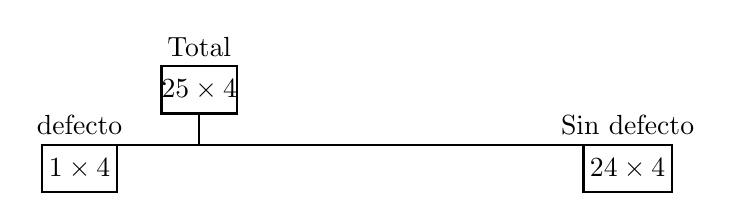
\begin{tikzpicture}[x=0.08cm,y=1cm]
		
		% línea principal
		\draw[thick] (0,1.6) -- (100,1.6);
		
		% marca central
		\draw[thick] (25,1.6) -- (25,2.0);
		
		% cuadro total
		\draw[thick] (19,2.0) rectangle (31,2.6);
		\node at (25,2.3) {$25\times 4$};
		\node at (25,2.85) {Total};
		
		% cuadro defecto
		\draw[thick] (0,1.0) rectangle (12,1.6);
		\node at (6,1.3) {$1\times 4$};
		\node at (6,1.85) {defecto};
		
		% cuadro sin defecto
		\draw[thick] (86,1.0) rectangle (100,1.6);
		\node at (93,1.3) {$24\times 4$};
		\node at (93,1.85) {Sin defecto};
		
	\end{tikzpicture}
	
	
	Luego
	
	$(n^\circ \text{ de casos Totales})=(n^\circ \text{ total de Televisores})=100$
	
	Además
	
	$(n^\circ \text{ de casos favorables})=(n^\circ \text{ de Televisores con defecto})=4$
	
	$\Rightarrow (\text{probabilidad pedida})=\dfrac{4}{100}=\dfrac{1}{25}$\fbox{$=4\%$}
	
	\vspace{6mm}
	
\end{enumerate}





\subsection*{Álgebra}

\begin{enumerate}[resume]
	
	\item ¿Cuántos términos del desarrollo de $(3\sqrt{3}+\sqrt{2})^{12}$ son números naturales?
	\begin{enumerate}[label=\alph*)]
		\item 7
		\item 6
		\item 3
		\item 4
		\item 5
	\end{enumerate}
	\textbf{Respuesta correcta:} a)
	
	\vspace{2mm}
	\textbf{Solucionario:}\\[1mm]
	
	$T_{k+1}=C_k^{12}a^{12-k}\cdot b^k$
	
	$\therefore\ T_{k+1}=C_k^{12}(3\sqrt{3})^{12-k}\cdot (\sqrt{2})^k$
	
	$=C_k^{12}\,3^{12-k}\cdot 3^{\dfrac{12-k}{2}}\cdot 2^{\dfrac{k}{2}}$
	
	Los valores $\dfrac{12-k}{2}$ y $\dfrac{k}{2}$ deben ser pares.
	
	\fbox{$\therefore\ k=\{0,2,4,6,8,10,12\}$}
	
	de donde 7 términos del desarrollo son números naturales.
	
	\vspace{6mm}
	
	\item Sean los polinomios $P(x)=2x^2-15$ y $Q(x,y)=2x+3y-2$. Halle el término independiente del polinomio $H(t)=Q(P(3),3t-1)$
	\begin{enumerate}[label=\alph*)]
		\item $-5$
		\item $-15$
		\item $-2$
		\item $1$
		\item $7$
	\end{enumerate}
	\textbf{Respuesta correcta:} d)
	
	\vspace{2mm}
	\textbf{Solucionario:}\\[1mm]
	
	$P(3)=2(3)^2-15=3$
	
	$H(t)=Q(3,3t-1)=2(3)+3(3t-1)-2$
	
	$=6+9t-3-2$
	
	$=9t+1$
	
	\fbox{$H(0)=1$} 
	
	\vspace{6mm}
	
	\item Dada la función $f(x)=4|x|-x^2,\ \ x\in\langle -4,4\rangle$ halle el valor de verdad de las siguientes proposiciones.
	
	I. $f(x)$ es una función impar.\\
	II. Para $x\geq 0$ en el dominio de la función, la gráfica de $f$ es una parábola que se abre hacia abajo.\\
	III. La gráfica de $f$ es simétrica respecto al eje $Y$.
	
	\begin{enumerate}[label=\alph*)]
		\item FVV
		\item FFF
		\item VFF
		\item VFV
		\item FVF
	\end{enumerate}
	\textbf{Respuesta correcta:} a)
	
	\vspace{2mm}
	\textbf{Solucionario:}\\[1mm]
	
	I. $f(-x)=4|-x|-(-x)^2=4x-x^2=f(x)$ \hfill (F)
	
	II. Si $x\geq 0 \Rightarrow f(x)=4x-x^2$ es una parábola que se abre hacia abajo \hfill (V)
	
	III. $f$ es par, por tanto hay simetría respecto al eje $Y$ \hfill (V)
	
	\vspace{6mm}
	
\end{enumerate}






\subsection*{Geometría}

\begin{enumerate}[resume]
	
	\item En la figura: \hspace{2mm} $AB=BD$, \hspace{2mm} $m\angle ACD=40^\circ$, \hspace{2mm} $m\angle BAC=m\angle CAD$ \hspace{2mm} y \hspace{2mm} $m\angle BDC=m\angle CDE$.\\
	Calcule $x$.
	
	\begin{center}
		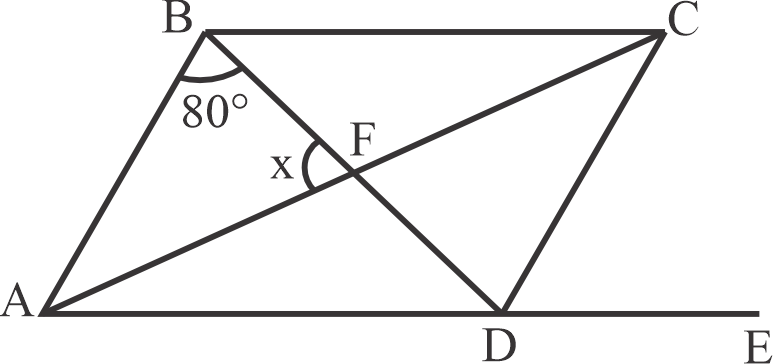
\includegraphics[width=4.5cm]{imagenes/general2024-I/etapa1/soc/geo1g24-I.png}
	\end{center}
	
	\begin{enumerate}[label=\alph*)]
		\item $75^\circ$
		\item $65^\circ$
		\item $30^\circ$
		\item $45^\circ$
		\item $60^\circ$
	\end{enumerate}
	\textbf{Respuesta correcta:} a)
	
	\vspace{2mm}
	\textbf{Solucionario:}\\[1mm]
	
	
	
		\begin{center}
		\begin{minipage}{0.45\textwidth}
		de la fig.
	
		$\bullet\ \ 4\alpha=180-80 \ \ \Rightarrow\ \ \alpha=25$
		
		$\bullet\ \ 3\alpha=x$
		
		$3(25)=x$
		
		\fbox{$75^\circ=x$}
			\vspace{6mm}
		\end{minipage}
		\hfill
		\begin{minipage}{0.45\textwidth}
			\centering
			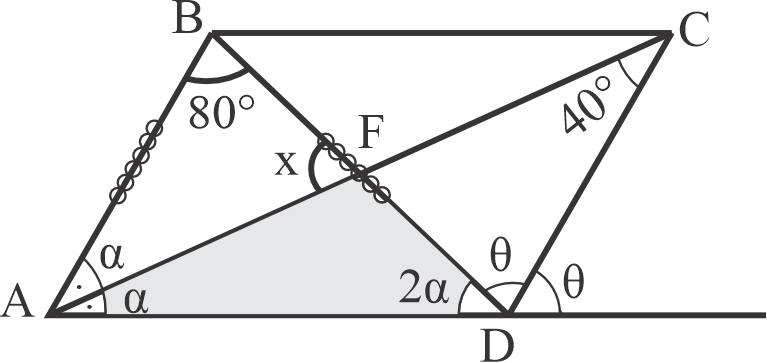
\includegraphics[width=4.5cm]{imagenes/general2024-I/etapa1/soc/geo1g24-Ir.png}
		\end{minipage}
	\end{center}
	
	
	\vspace{6mm}
	
	\item Halle el valor de verdad de las siguientes proposiciones:
	
	I. Un ángulo obtuso es aquel cuya medida es comprendida entre $0^\circ$ y $90^\circ$\\
	II. Los ángulos suplementarios son aquellos cuyas medidas suman $90^\circ$\\
	III. La intersección de las medianas de un triángulo se llama Incentro.\\
	IV. La cuerda mayor de una circunferencia se llama diámetro.
	
	\begin{enumerate}[label=\alph*)]
		\item VFVF
		\item FVFV
		\item FFVV
		\item VVFF
		\item FFFV
	\end{enumerate}
	\textbf{Respuesta correcta:} e)
	
	\vspace{2mm}
	\textbf{Solucionario:}\\[1mm]
	
	I) $\alpha$ es obtuso, por lo tanto \hfill (F)
	
	II) Ángulos suplementarios es: $180^\circ$ \hfill (F)
	
	III) no es incentro, se llama baricentro \hfill (F)
	
	IV) $D=$ cuerda mayor. \hfill (V)
	
	\vspace{6mm}
	
\end{enumerate}




\subsection*{Trigonometría}

\begin{enumerate}[resume]
	
	\item En la figura, calcule la longitud del segmento $BC$, si $\sen\alpha=0,5$ y $AD=5$
	
	\begin{center}
		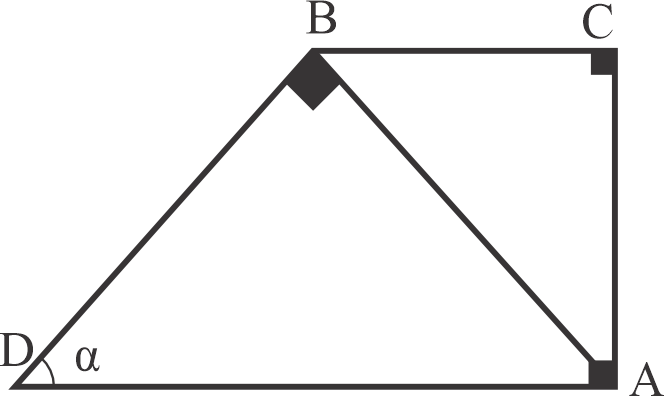
\includegraphics[width=4.3cm]{imagenes/general2024-I/etapa1/soc/trigo1g24-I.png}
	\end{center}
	
	\begin{enumerate}[label=\alph*)]
		\item $\dfrac{8}{5}$
		\item $\dfrac{10}{3}$
		\item $\dfrac{5}{4}$
		\item $\dfrac{3}{4}$
		\item $\dfrac{7}{6}$
	\end{enumerate}
	\textbf{Respuesta correcta:} c)
	
	\vspace{2mm}
	\textbf{Solucionario:}\\[1mm]

	
	\begin{center}
		\begin{minipage}{0.45\textwidth}
		$x=(5\sen\alpha)(\sen\alpha)$
	
		$=5\sen^2\alpha$
		
		$=5\left(\dfrac{1}{2}\right)^2$
	
		\fbox{$=\dfrac{5}{4}$}
			
			
			\vspace{6mm}
		\end{minipage}
		\hfill
		\begin{minipage}{0.45\textwidth}
			\centering
			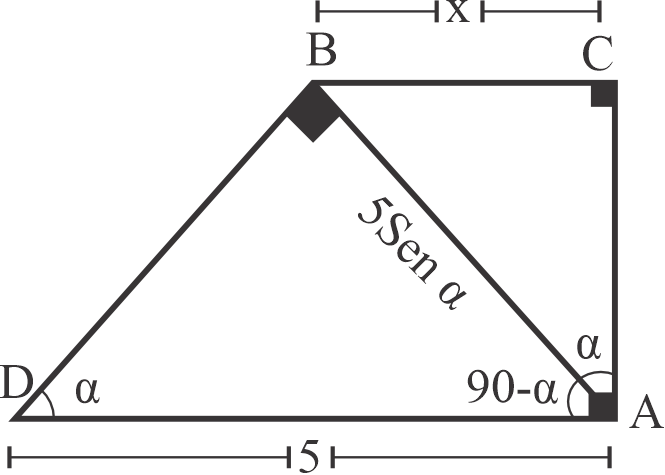
\includegraphics[width=4.3cm]{imagenes/general2024-I/etapa1/soc/trigo1g24-Ir.png}
		\end{minipage}
	\end{center}
	
	
	
	
	\vspace{6mm}
	
	\item Si $\alpha$ es un ángulo en el primer cuadrante y $\sin\alpha=0,25$ halle $\csc\alpha+\cot^2\alpha$
	
	\begin{enumerate}[label=\alph*)]
		\item $16$
		\item $\dfrac{9}{5}$
		\item $\dfrac{7}{8}$
		\item $19$
		\item $\dfrac{3}{8}$
	\end{enumerate}
	\textbf{Respuesta correcta:} d)
	
	\vspace{2mm}
	\textbf{Solucionario:}\\[1mm]
	

	
		\begin{center}
		\begin{minipage}{0.45\textwidth}
			$\csc\alpha+\cot^2\alpha$
			
			$=\dfrac{4}{1}+\left(\dfrac{\sqrt{15}}{1}\right)^2$
			
			$=4+15$
			
			\fbox{$=19$}
			
			
			\vspace{6mm}
		\end{minipage}
		\hfill
		\begin{minipage}{0.45\textwidth}
			\centering
			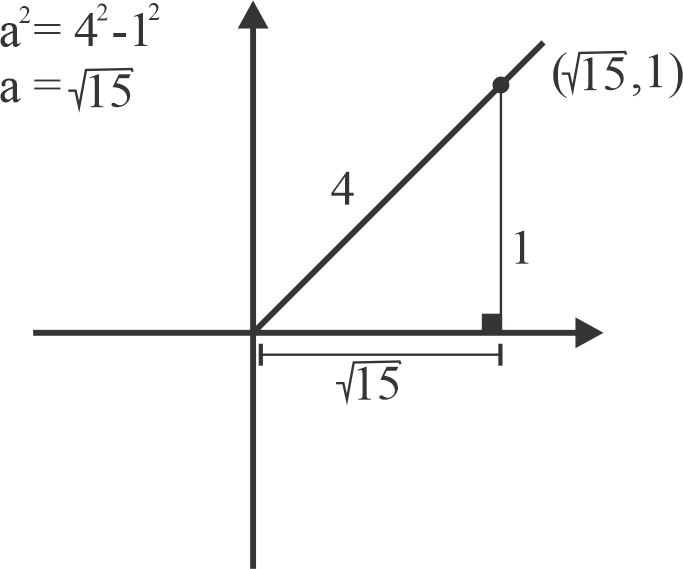
\includegraphics[width=4.5cm]{imagenes/general2024-I/etapa1/soc/trigo2g24-Ir.png}
		\end{minipage}
		\end{center}
	
	\vspace{6mm}
	
\end{enumerate}




\subsection*{Física}

\begin{enumerate}[resume]
	
\item Se tiene una puerta de plancha de acero de $300\ cm$ de largo y $200\ cm$ de alto a una temperatura de $0^\circ C$. Calcule el aumento de su área cuando el sol calienta hasta una temperatura de $100^\circ C$.

$(\alpha_{acero}=1{,}2\times10^{-5}\ ^\circ C^{-1})$

\begin{enumerate}[label=\alph*)]
	\item $141\ cm^2$
	\item $144\ cm^2$
	\item $143\ cm^2$
	\item $140\ cm^2$
	\item $142\ cm^2$
\end{enumerate}
\textbf{Respuesta correcta:} b)

\vspace{2mm}
\textbf{Solucionario:}\\[1mm]

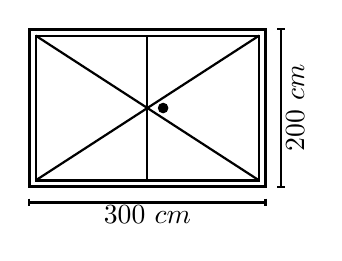
\begin{tikzpicture}[x=0.01cm,y=0.01cm]
	
	% Marco exterior de la puerta
	\draw[very thick] (0,0) rectangle (300,200);
	
	% Borde interno
	\draw[thick] (8,8) rectangle (292,192);
	
	% División central
	\draw[thick] (150,8) -- (150,192);
	
	% Detalles diagonales tipo panel
	\draw[thick] (8,8) -- (150,100);
	\draw[thick] (150,100) -- (292,192);
	
	\draw[thick] (8,192) -- (150,100);
	\draw[thick] (150,100) -- (292,8);
	
	% Perilla
	\filldraw[black] (170,100) circle (6);
	
	% Medidas
	\draw[thick] (0,-20) -- (300,-20);
	\draw[thick] (0,-15) -- (0,-25);
	\draw[thick] (300,-15) -- (300,-25);
	\node at (150,-35) {$300\ cm$};
	
	\draw[thick] (320,0) -- (320,200);
	\draw[thick] (315,0) -- (325,0);
	\draw[thick] (315,200) -- (325,200);
	\node[rotate=90] at (338,100) {$200\ cm$};
	
	\end{tikzpicture}

Área inicial:

$A_0=(300)(200)=60000\ cm^2$

$A_0=6\times10^4\ cm^2$

Cambio de temperatura:

$\Delta T=100^\circ C-0^\circ C=100^\circ C$

Para dilatación superficial:

$\beta=2\alpha$

$\beta=2(1{,}2\times10^{-5})$

$\beta=2{,}4\times10^{-5}\ ^\circ C^{-1}$

Usamos:

$\beta=\dfrac{\Delta A}{A_0\Delta T}$


$\Delta A=\beta A_0\Delta T$


$\Delta A=(2{,}4\times10^{-5})(6\times10^4)(100)$

$\Delta A=(2{,}4)(6)(10^{-5+4})(100)$

$\Delta A=14{,}4(10^{-1})(100)$

$\Delta A=1{,}44(100)$

\fbox{$\Delta A=144\ cm^2$}

\vspace{6mm}
	
	
	
	
	\item Una pelota de $0{,}5\ kg$ atada a una cuerda de $0{,}5\ m$ de radio gira uniformemente en un plano vertical con una rapidez tangencial de $10\ m/s$. Determine el módulo de la tensión de la cuerda en la posición más alta de su trayectoria. $(g=10\ m/s^2)$
	
	\begin{enumerate}[label=\alph*)]
		\item $90\ N$
		\item $92\ N$
		\item $95\ N$
		\item $94\ N$
		\item $93\ N$
	\end{enumerate}
	\textbf{Respuesta correcta:} c)
	
	\vspace{2mm}
	\textbf{Solucionario:}\\[1mm]
	
	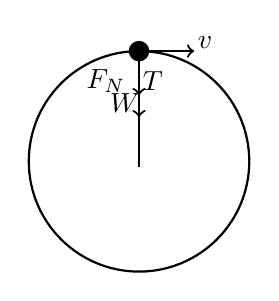
\begin{tikzpicture}[scale=0.7]
		\draw[thick] (0,0) circle (2);
		\filldraw[black] (0,2) circle (5pt);
		\draw[->, thick] (0,2) -- (0,0.8);
		\draw[->, thick] (0,2) -- (0,1.2);
		\draw[->, thick] (0,2) -- (1,2);
		\draw[-, thick] (0,2) -- (0,-0.1);
		\node at (0.25,1.45) {$T$};
		\node at (-0.60,1.45) {$F_N$};
		\node at (-0.25,1.05) {$W$};
		\node at (1.2,2.15) {$v$};
	\end{tikzpicture}
	
	
	$\sum F_c=T+W=\dfrac{mv^2}{R}$
	
	$\sum F_c=T+mg=\dfrac{mv^2}{R}$
	
	
	$T=\dfrac{mv^2}{R}-mg$
	
	$T=m\left(\dfrac{v^2}{R}-g\right)$
	
	$m=0{,}5\ kg,\qquad v=10\ m/s,\qquad R=0{,}5\ m,\qquad g=10\ m/s^2$
	
	$T=0{,}5\left(\dfrac{10^2}{0{,}5}-10\right)$
	
	$T=0{,}5\left(\dfrac{100}{0{,}5}-10\right)$
	
	$T=0{,}5(200-10)$
	
	$T=0{,}5(190)$
	
	\fbox{$T=95\ N$}
	
	\vspace{6mm}
	
	
	
	
	
	
\end{enumerate}


\subsection*{Química}

\begin{enumerate}[resume]
	
	\item Indique las propiedades químicas del carbono.
	
	I. tetravalencia\\
	II. covalencia\\
	III. peso específico\\
	IV. autosaturación
	
	\begin{enumerate}[label=\alph*)]
		\item I, II y III
		\item II, III y IV
		\item III y IV
		\item I, II y IV
		\item II y IV
	\end{enumerate}
	\textbf{Respuesta correcta:} d)
	
	\vspace{2mm}
	\textbf{Solucionario:}\\[1mm]
	
	Las propiedades químicas del átomo de carbono son:
	
	I) tetravalencia.\\
	II) covalencia.\\
	IV) autosaturación.
	
	No se considera el peso específico como propiedad química.
	
	\vspace{6mm}
	
	\item Determine el volumen de 1 mol de una sustancia a la presión de $1,5$ atmósferas y $27^\circ C$
	
	\begin{enumerate}[label=\alph*)]
		\item $13,6L$
		\item $17,4L$
		\item $14,6L$
		\item $15,4L$
		\item $16,4L$
	\end{enumerate}
	\textbf{Respuesta correcta:} e)
	
	\vspace{2mm}
	\textbf{Solucionario:}\\[1mm]
	
	Datos
	
	$P=1,5\ atm$
	
	$R\text{ constante}=0.082\ \dfrac{L\cdot atm}{mol\cdot K}$
	
	$T=27^\circ C=300^\circ K$
	
	$\Rightarrow$ si \hspace{2mm} $PV=nRT$
	
	despejando el $V=\dfrac{nRT}{P}$
	
	$V=\dfrac{1\ mol\cdot 0.082\ \dfrac{L\cdot atm}{mol\cdot K}\cdot 300^\circ K}{1.5\ atm}$
	
	\fbox{$V=16.4\ L$}
	
	\vspace{6mm}
	
\end{enumerate}





\subsection*{Biología y Anatomía}

\begin{enumerate}[resume]
	
	\item La relación estrecha entre dos especies en la cual la evolución de una promueve la evolución de la otra, hasta llegar a un estado de interdependencia, se denomina:
	\begin{enumerate}[label=\alph*)]
		\item Evolución adaptativa
		\item Evolución paralela
		\item Evolución advergente
		\item Coevolución
		\item Convergencia evolutiva
	\end{enumerate}
	\textbf{Respuesta correcta:} d)
	
	\vspace{2mm}
	\textbf{Solucionario:}\\[1mm]
	La \textbf{coevolución} ocurre cuando dos especies interactúan de manera tan estrecha que los cambios evolutivos en una influyen en la otra, generando interdependencia.
	
	\vspace{6mm}
	
	\item ¿Cuál es el conducto que se dirige hacia el duodeno y desemboca junto con el conducto pancreático, en el área denominada ampolla Vater?
	\begin{enumerate}[label=\alph*)]
		\item De Herring
		\item Hepático común
		\item Cístico
		\item Colédoco
		\item De Wharton
	\end{enumerate}
	\textbf{Respuesta correcta:} d)
	
	\vspace{2mm}
	\textbf{Solucionario:}\\[1mm]
	El \textbf{conducto colédoco} transporta la bilis hacia el duodeno y se une con el conducto pancreático en la ampolla de Vater.
	
	\vspace{6mm}
	
\end{enumerate}

\subsection*{Psicología y Filosofía}

\begin{enumerate}[resume]
	
	
	\item Un niño aprende que, si llora, su mamá le prestará atención y lo mimará inclusive le dará un caramelo “Para que se sienta mejor”. En este caso, el niño controla perfectamente la situación y su entorno.\\
	Este comportamiento corresponde al condicionamiento:
	\begin{enumerate}[label=\alph*)]
		\item Placentero.
		\item Operante
		\item Experimental
		\item Clásico
		\item Reforzado
	\end{enumerate}
	\textbf{Respuesta correcta:} b)
	
	\vspace{2mm}
	\textbf{Solucionario:}\\[1mm]
	Es \textbf{condicionamiento operante} porque el niño realiza una conducta y obtiene una consecuencia favorable, reforzando ese comportamiento.
	
	\vspace{6mm}
	
	\item En la actualidad, un porcentaje elevado de personas realizan simultáneamente dos cosas. Por ejemplo, escribir y contestar el teléfono. En este caso, se hace uso de la atención.
	\begin{enumerate}[label=\alph*)]
		\item Refleja
		\item Dividida
		\item Selectiva
		\item Sostenida
		\item Automática
	\end{enumerate}
	\textbf{Respuesta correcta:} b)
	
	\vspace{2mm}
	\textbf{Solucionario:}\\[1mm]
	La \textbf{atención dividida} permite atender dos tareas al mismo tiempo.
	
	\vspace{6mm}
	
	\item Adriana es mucho más bella que María. ¿Qué característica del valor se resalta en el enunciado anterior?
	\begin{enumerate}[label=\alph*)]
		\item Subjetivo
		\item Objetivo
		\item Gradual
		\item Jerárquico
		\item Polaridad
	\end{enumerate}
	\textbf{Respuesta correcta:} c)
	
	\vspace{2mm}
	\textbf{Solucionario:}\\[1mm]
	La expresión “mucho más” indica una comparación por grados, por eso corresponde a la característica \textbf{gradual} del valor.
	
	\vspace{6mm}
	
	\item Sergio manifiesta que el hombre es libre de hacer lo que desea y sin límites. Ante lo dicho por Sergio, Kant manifestaría que:
	\begin{enumerate}[label=\alph*)]
		\item Se equivoca, ya que él vive dentro de una sociedad y él está determinado por ella.
		\item Tiene razón y por ello puede actuar sin consciencia, pero si con libertad.
		\item Se equivoca, puesto que el hombre no tiene libertad de ir contra la naturaleza ni contra la sociedad.
		\item No tiene razón y que debe guiarse por la experiencia de los demás y buscar su beneficio.
		\item No se equivoca, pues puede hacer lo que desee, pero su guía debe de ser la razón.
	\end{enumerate}
	\textbf{Respuesta correcta:} e)
	
	\vspace{2mm}
	\textbf{Solucionario:}\\[1mm]
	Para Kant, la libertad debe estar guiada por la \textbf{razón} y la ley moral. Por ello, la opción marcada es la que mejor se ajusta.
	
	\vspace{6mm}
	
\end{enumerate}

\subsection*{Geografía}

\begin{enumerate}[resume]

	
	\item Los bordes de las placas son zonas con una gran actividad tectónica, que se manifiestan mediante:
	\begin{enumerate}[label=\alph*)]
		\item Vientos huracanados
		\item Fenómenos geológicos
		\item Fenómenos atmosféricos
		\item Movimientos de la tierra
		\item Actividades volcánicas y terremotos
	\end{enumerate}
	\textbf{Respuesta correcta:} e)
	
	\vspace{2mm}
	\textbf{Solucionario:}\\[1mm]
	En los bordes de placas predominan \textbf{volcanes y terremotos}, pues allí se concentra la dinámica tectónica.
	
	\vspace{6mm}
	
	\item El yacimiento mineral de Litio que se encuentra en la Región de Puno corresponde a los:
	\begin{enumerate}[label=\alph*)]
		\item Recursos naturales inagotables
		\item Recursos naturales renovables
		\item Recursos naturales no renovables
		\item Recursos naturales vitales
		\item Recursos naturales superfluos
	\end{enumerate}
	\textbf{Respuesta correcta:} c)
	
	\vspace{2mm}
	\textbf{Solucionario:}\\[1mm]
	El litio es un recurso mineral, por tanto es un \textbf{recurso natural no renovable}.
	
	\vspace{6mm}
	
	\item El eje polar o axial es una línea imaginaria terrestre, también denominado:
	\begin{enumerate}[label=\alph*)]
		\item El eje terrestre
		\item La línea ecuatorial
		\item Los paralelos
		\item Los meridianos
		\item Las coordenadas
	\end{enumerate}
	\textbf{Respuesta correcta:} a)
	
	\vspace{2mm}
	\textbf{Solucionario:}\\[1mm]
	El eje polar o axial también recibe el nombre de \textbf{eje terrestre}.
	
	\vspace{6mm}
	
	\item Últimamente hay un aumento en la intensidad de los fenómenos naturales sobre la tierra. Esto sucede por:
	\begin{enumerate}[label=\alph*)]
		\item La deforestación
		\item El cambio climático
		\item La lluvia ácida
		\item La contaminación del agua
		\item La desertificación
	\end{enumerate}
	\textbf{Respuesta correcta:} b)
	
	\vspace{2mm}
	\textbf{Solucionario:}\\[1mm]
	El \textbf{cambio climático} incrementa la intensidad y frecuencia de diversos fenómenos naturales.
	
	\vspace{6mm}
	
\end{enumerate}

\subsection*{Historia}

\begin{enumerate}[resume]

	
	\item Los restos fósiles conocidos como “Lucy” pertenecen a homínido de andar erecto. Fueron clasificados dentro del género Australopithecus y la especie…
	\begin{enumerate}[label=\alph*)]
		\item Anamensis
		\item Ramidus
		\item Africanus
		\item Afarensis
		\item Habilis
	\end{enumerate}
	\textbf{Respuesta correcta:} d)
	
	\vspace{2mm}
	\textbf{Solucionario:}\\[1mm]
	Lucy pertenece a la especie \textbf{Australopithecus afarensis}.
	
	\vspace{6mm}
	
	\item Las juntas de Gobierno surgidas tanto en España como en América para defender los derechos del Rey Fernando VII, tuvieron como origen el vacío político ocasionado por \rule{3cm}{0.4pt} 1808 y 1813.
	\begin{enumerate}[label=\alph*)]
		\item La guerra entre Inglaterra y Francia, siendo España aliada de Francia.
		\item La invasión de España por el ejército napoleónico
		\item La invasión de Napoleón a México
		\item Las expediciones militares inglesas contra Buenos Aires
		\item El rechazo a la Constitución Cádiz
	\end{enumerate}
	\textbf{Respuesta correcta:} b)
	
	\vspace{2mm}
	\textbf{Solucionario:}\\[1mm]
	Las juntas surgieron como respuesta a \textbf{la invasión napoleónica de España}, que generó un vacío de poder.
	
	\vspace{6mm}
	
	\item La domesticación de plantas fue uno de los principales hitos en la historia de la humanidad. En los Andes, el sitio arqueológico de \rule{3cm}{0.4pt} (ca. 7500 a.n.e.) es considerado como el yacimiento hortícola de mayor antigüedad, donde se hallaron restos de frijoles, pallares y calabazas.
	\begin{enumerate}[label=\alph*)]
		\item Guitarrero
		\item Chilca
		\item Telarmachay
		\item Piquimachay
		\item Lauricocha
	\end{enumerate}
	\textbf{Respuesta correcta:} a)
	
	\vspace{2mm}
	\textbf{Solucionario:}\\[1mm]
	El yacimiento hortícola más antiguo señalado es \textbf{Guitarrero}.
	
	\vspace{6mm}
	
	\item A la subdivisión territorial de las audiencias encargadas del control centralista del latifundismo y la representación de la corona en las comunidades andinas se denominó:
	\begin{enumerate}[label=\alph*)]
		\item Cabildos
		\item Corregimientos
		\item Capitanías
		\item Reducciones
		\item Intendencias
	\end{enumerate}
	\textbf{Respuesta correcta:} b)
	
	\vspace{2mm}
	\textbf{Solucionario:}\\[1mm]
	Esas subdivisiones territoriales coloniales se llamaron \textbf{corregimientos}.
	
	\vspace{6mm}
	
\end{enumerate}

\subsection*{Educación Cívica}

\begin{enumerate}[resume]

	
	\item Según el Régimen de Sucesión de Bienes, se considera heredero forzoso a:
	\begin{enumerate}[label=\alph*)]
		\item Hermanos
		\item Cónyuges
		\item Sobrinos
		\item Tíos
		\item Primos hermanos
	\end{enumerate}
	\textbf{Respuesta correcta:} b)
	
	\vspace{2mm}
	\textbf{Solucionario:}\\[1mm]
	Entre las opciones, el \textbf{cónyuge} es heredero forzoso.
	
	\vspace{6mm}
	
	\item Edgar y María deciden mediante contrato privado realizar una promesa para contraer matrimonio en noviembre del 2024. Este acto corresponde:
	\begin{enumerate}[label=\alph*)]
		\item Al concubinato
		\item A la unión de hecho
		\item Al matrimonio
		\item A los esponsales
		\item Al noviazgo
	\end{enumerate}
	\textbf{Respuesta correcta:} d)
	
	\vspace{2mm}
	\textbf{Solucionario:}\\[1mm]
	La promesa formal de matrimonio corresponde a los \textbf{esponsales}.
	
	\vspace{6mm}
	
	\item Uno de los fines principales de la ONU es:
	\begin{enumerate}[label=\alph*)]
		\item Solución pacífica de conflictos
		\item Promover el desarrollo equilibrado y armónico
		\item Mantener la paz mundial
		\item Defensa de la libertad y soberanía
		\item Acelerar el crecimiento económico
	\end{enumerate}
	\textbf{Respuesta correcta:} c)
	
	\vspace{2mm}
	\textbf{Solucionario:}\\[1mm]
	Uno de los fines esenciales de la ONU es \textbf{mantener la paz mundial}.
	
	\vspace{6mm}
	
	\item La \rule{3cm}{0.4pt} procede por infracción de la Constitución y de la Ley, contra reglamentos, normas administrativas y resoluciones y decretos de carácter general, cualquiera sea la autoridad que emanen.
	\begin{enumerate}[label=\alph*)]
		\item Acción de cumplimiento
		\item Acción popular
		\item Acción de Hábeas Data
		\item Acción de Inconstitucionalidad
		\item Acción de Amparo
	\end{enumerate}
	\textbf{Respuesta correcta:} b)
	
	\vspace{2mm}
	\textbf{Solucionario:}\\[1mm]
	La garantía que procede contra reglamentos y normas generales por infracción constitucional o legal es la \textbf{acción popular}.
	
	\vspace{6mm}
	
\end{enumerate}

\subsection*{Economía}

\begin{enumerate}[resume]

	
	\item María y Rodrigo acuden a un mercado de Puno con la intención de adquirir polos para sus hijos de 4 y 13 años, respectivamente. Al llegar a la sección de vestimenta, observan un panel muy atractivo que hace referencia a una nueva marca de polos para niños que, por el diseño y los dibujos de conocidos personajes, es de gran preferencia del público infantil, por lo que deciden adquirir ropa de dicha marca. De esta experiencia, se puede afirmar que:
	\begin{enumerate}[label=\alph*)]
		\item La edad determina el comportamiento del consumidor
		\item La conducta del consumidor depende del costo de producción
		\item El precio del bien depende de la cantidad demandada
		\item La demanda depende de la cantidad de bienes que se ofrecen
		\item La publicidad es un factor que influye en la cantidad de demanda
	\end{enumerate}
	\textbf{Respuesta correcta:} e)
	
	\vspace{2mm}
	\textbf{Solucionario:}\\[1mm]
	El panel y el atractivo de la marca muestran que la \textbf{publicidad} influye en la demanda.
	
	\vspace{6mm}
	
	\item El costo \rule{2cm}{0.4pt} permite derivar la curva de la \rule{2cm}{0.4pt} en un mercado de competencia perfecta.
	\begin{enumerate}[label=\alph*)]
		\item Medio – producción
		\item Marginal – oferta
		\item Unitario – oferta
		\item Social – eficiencia
		\item Variable – demanda
	\end{enumerate}
	\textbf{Respuesta correcta:} b)
	
	\vspace{2mm}
	\textbf{Solucionario:}\\[1mm]
	En competencia perfecta, la curva de \textbf{oferta} se deriva del costo \textbf{marginal}.
	
	\vspace{6mm}
	
	\item De acuerdo a la teoría económica, una diferencia entre el mercado de competencia perfecta y el de comportamiento imperfecto es que en este último
	\begin{enumerate}[label=\alph*)]
		\item No existe poder de mercado
		\item El precio siempre es mayor
		\item Predomina la oferta y la demanda
		\item El Estado necesariamente establece el precio de equilibrio
		\item Se genera un menor bienestar para la sociedad
	\end{enumerate}
	\textbf{Respuesta correcta:} e)
	
	\vspace{2mm}
	\textbf{Solucionario:}\\[1mm]
	En los mercados imperfectos suele generarse \textbf{menor bienestar social} por ineficiencias y poder de mercado.
	
	\vspace{6mm}
	
	\item El estancamiento de la producción, del consumo, del ahorro y de la inversión se manifiesta en la fase del ciclo económico denominada:
	\begin{enumerate}[label=\alph*)]
		\item Crisis
		\item Reanimación
		\item Reactivación
		\item Depresión
		\item Recesión
	\end{enumerate}
	\textbf{Respuesta correcta:} e)
	
	\vspace{2mm}
	\textbf{Solucionario:}\\[1mm]
	El estancamiento de esas variables caracteriza la \textbf{recesión}.
	
	\vspace{6mm}
	
\end{enumerate}

\subsection*{Comunicación}

\begin{enumerate}[resume]

	
	\item Tal vez parezca paradójico lo que voy a decir, pero es verdad. Lo que peor nos ha ocurrido en el pasado, es lo mejor para el futuro ¿Qué es esto? Que la situación es grave porque no habéis hecho nada, ni poco ni mucho.\\
	¿A qué tipo de texto corresponde el fragmento?
	\begin{enumerate}[label=\alph*)]
		\item Argumentativo
		\item Expositivo
		\item Narrativo
		\item Descriptivo
		\item Instructivo
	\end{enumerate}
	\textbf{Respuesta correcta:} a)
	
	\vspace{2mm}
	\textbf{Solucionario:}\\[1mm]
	El fragmento presenta una postura y razones, por eso corresponde a un texto \textbf{argumentativo}.
	
	\vspace{6mm}
	
	\item Margarita llega al salón de clases y escucha atentamente al profesor y decide escribir las ideas más importantes.\\
	¿Qué técnica de estudio utiliza Margarita?
	\begin{enumerate}[label=\alph*)]
		\item Subrayado
		\item Toma de apuntes
		\item Sumillado
		\item Esquema
		\item Resumen
	\end{enumerate}
	\textbf{Respuesta correcta:} b)
	
	\vspace{2mm}
	\textbf{Solucionario:}\\[1mm]
	Escribir las ideas principales mientras escucha corresponde a la \textbf{toma de apuntes}.
	
	\vspace{6mm}
	
	\item Es el momento donde las ideas se expresan en un lenguaje visible, lineal, que debe ajustarse a las convenciones de la lengua escrita.\\
	¿A qué etapa del proceso de la escritura corresponde?
	\begin{enumerate}[label=\alph*)]
		\item Problematización
		\item Organización
		\item Redacción
		\item Planificación
		\item Revisión
	\end{enumerate}
	\textbf{Respuesta correcta:} c)
	
	\vspace{2mm}
	\textbf{Solucionario:}\\[1mm]
	Esa etapa es la \textbf{redacción}, donde las ideas ya se expresan por escrito.
	
	\vspace{6mm}
	
	\item “Mi país, ahora lo comprendo, es amargo y dulce”.\\
	El texto utiliza un lenguaje:
	\begin{enumerate}[label=\alph*)]
		\item Connotativo
		\item Denotativo
		\item Coloquial
		\item Literario
		\item Científico
	\end{enumerate}
	\textbf{Respuesta correcta:} a)
	
	\vspace{2mm}
	\textbf{Solucionario:}\\[1mm]
	La expresión tiene sentido figurado, por lo que utiliza lenguaje \textbf{connotativo}.
	
	\vspace{6mm}
	
\end{enumerate}

\subsection*{Literatura}

\begin{enumerate}[resume]

	
	\item Tengo miedo de verte necesidad de verte esperanza de verte desazones de verte\\
	La reiteración de la última palabra de cada verso se denomina
	\begin{enumerate}[label=\alph*)]
		\item Metáfora
		\item Anáfora
		\item Eufemismo
		\item Complexión
		\item Epifora
	\end{enumerate}
	\textbf{Respuesta correcta:} e)
	
	\vspace{2mm}
	\textbf{Solucionario:}\\[1mm]
	La repetición al final de cada verso se llama \textbf{epífora}.
	
	\vspace{6mm}
	
	\item ¿Quién es el escritor que hace uso del caligrama?
	\begin{enumerate}[label=\alph*)]
		\item Martín Adán
		\item César Vallejo
		\item Arturo Peralta
		\item Carlos Oquendo de Amat
		\item Dante Nava
	\end{enumerate}
	\textbf{Respuesta correcta:} d)
	
	\vspace{2mm}
	\textbf{Solucionario:}\\[1mm]
	El escritor vinculado al uso del \textbf{caligrama} es \textbf{Carlos Oquendo de Amat}.
	
	\vspace{6mm}
	
	\item Rumi Ñawi en la obra literaria Ollantay, asume el significado de:
	\begin{enumerate}[label=\alph*)]
		\item Gran guerrero
		\item Ojos de piedra
		\item Cazador de pobres
		\item Vengador del inca
		\item Fortaleza inca
	\end{enumerate}
	\textbf{Respuesta correcta:} b)
	
	\vspace{2mm}
	\textbf{Solucionario:}\\[1mm]
	“Rumi Ñawi” significa \textbf{ojos de piedra}.
	
	\vspace{6mm}
	
	\item “El Cid se dirige al mediterráneo y toma la posición de Valencia. Los triunfos y ganancias del campeador crean codicias en los infantes de Carrión (Diego y Fernando) quienes solicitan casarse con las hijas del Cid…”.\\
	El fragmento corresponde a:
	\begin{enumerate}[label=\alph*)]
		\item La novela de caballería
		\item La epístola
		\item La epopeya heroica
		\item La sátira
		\item El Cantar de gesta
	\end{enumerate}
	\textbf{Respuesta correcta:} e)
	
	\vspace{2mm}
	\textbf{Solucionario:}\\[1mm]
	El fragmento pertenece al género épico medieval llamado \textbf{cantar de gesta}.
	
	\vspace{6mm}
	
\end{enumerate}


\subsection*{Razonamiento Matemático}

\begin{enumerate}[resume]
	
	\item Hace 55 años, Judit tenía la sexta parte de la edad que tiene ahora. ¿Cuántos años tendría si hubiese nacido 15 años después?
	\begin{enumerate}[label=\alph*)]
		\item 50
		\item 41
		\item 52
		\item 51
		\item 61
	\end{enumerate}
	\textbf{Respuesta correcta:} d)
	
	\vspace{2mm}
	\textbf{Solucionario:}\\[1mm]
	
	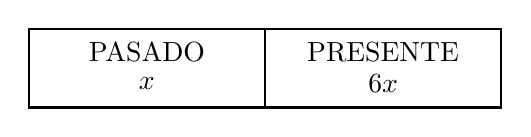
\begin{tikzpicture}
		\draw[thick] (0,0) rectangle (3,1);
		\draw[thick] (3,0) rectangle (6,1);
		\node at (1.5,0.7) {PASADO};
		\node at (4.5,0.7) {PRESENTE};
		\node at (1.5,0.3) {$x$};
		\node at (4.5,0.3) {$6x$};
	\end{tikzpicture}
	
	Se dan los datos
	
	$x+55=6x$
	
	$55=5x$
	
	$x=11$
	
	La edad actual es:
	
	\fbox{$6x=6(11)=66$}
	
	Si hubiese nacido 15 años después:
	
	$66-15=51$ años.
	
	\vspace{6mm}
	
	\item Si se sube una escalera de 4 en 4 escalones, se da 3 pasos más que subiendo de 5 en 5 escalones. ¿Cuántos escalones tiene la escalera?
	\begin{enumerate}[label=\alph*)]
		\item 40
		\item 60
		\item 56
		\item 62
		\item 80
	\end{enumerate}
	\textbf{Respuesta correcta:} b)
	
	\vspace{2mm}
	\textbf{Solucionario:}\\[1mm]
	
	\begin{tikzpicture}[scale=0.6]
		% escalera 4
		\draw[thick] (0,0) -- (4,0) -- (4,3);
		\draw[thick] (0,0)
		-- (0.3,0.3) -- (0.6,0.3) -- (0.6,0.6)
		-- (0.9,0.6) -- (0.9,0.9) -- (1.2,0.9)
		-- (1.2,1.2) -- (1.5,1.2) -- (1.5,1.5)
		-- (1.8,1.5) -- (1.8,1.8) -- (2.1,1.8)
		-- (2.1,2.1) -- (2.4,2.1) -- (2.4,2.4)
		-- (2.7,2.4) -- (2.7,2.7) -- (3,2.7)
		-- (3,3);
		\node at (2,-0.4) {$x$ escalones};

		\node at (2.7,3.1) {4 esc.};
		
	\node at (2,-1.4) {\# pasos $=\dfrac{x}{4}$};
		
		% escalera 5
		\begin{scope}[xshift=7cm]
			\draw[thick] (0,0) -- (4,0) -- (4,3);
			\draw[thick] (0,0)
			-- (0.25,0.25) -- (0.5,0.25) -- (0.5,0.5)
			-- (0.75,0.5) -- (0.75,0.75) -- (1,0.75)
			-- (1,1) -- (1.25,1) -- (1.25,1.25)
			-- (1.5,1.25) -- (1.5,1.5) -- (1.75,1.5)
			-- (1.75,1.75) -- (2,1.75) -- (2,2)
			-- (2.25,2) -- (2.25,2.25) -- (2.5,2.25)
			-- (2.5,2.5) -- (2.75,2.5) -- (2.75,2.75)
			-- (3,2.75) -- (3,3);
			\node at (2,-0.4) {$x$ escalones};
				\node at (2.6,3.1) {5 esc.};
			\node at (2,-1.4) {\# pasos $=\dfrac{x}{5}$};
		\end{scope}
	\end{tikzpicture}
	
	
	$\dfrac{x}{4}-\dfrac{x}{5}=3$
	
	\fbox{$x=60$ escalones.}
	
	\vspace{6mm}
	
	\item ¿Cuál es el número de 5 cifras que, multiplicado por 22, da un producto cuyas cifras son todas 8? Dé como respuesta la suma de cifras del número.
	\begin{enumerate}[label=\alph*)]
		\item 14
		\item 12
		\item 16
		\item 10
		\item 8
	\end{enumerate}
	\textbf{Respuesta correcta:} b)
	
	\vspace{2mm}
	\textbf{Solucionario:}\\[1mm]
	
	Sea un número de 5 cifras $\overline{abcde}$
	
	$\overline{abcde}\times 22=88\ldots 88$
	
	
	$\overline{abcde}=\dfrac{88\ldots 88}{22}$
	
	\begin{center}
		\(
		\Rightarrow \overline{abcde}=40404
		\)
	\end{center}
	
	
\fbox{	$4+0+4+0+4=12$}
	
	\vspace{6mm}
	
	\item Si se sabe que Manuel es mayor que Sara y Arturo, pero éste último es mayor que Vanesa y Sara. ¿Cuál de las siguientes afirmaciones no es verdadera?
	\begin{enumerate}[label=\alph*)]
		\item Sara es menor que Arturo
		\item Vanesa es menor que Arturo
		\item Manuel es menor que Arturo
		\item Sara es menor que Manuel
		\item Vanesa es menor que Manuel
	\end{enumerate}
	\textbf{Respuesta correcta:} c)
	
	\vspace{2mm}
	\textbf{Solucionario:}\\[1mm]
	
	\textit{i)} menor
	
	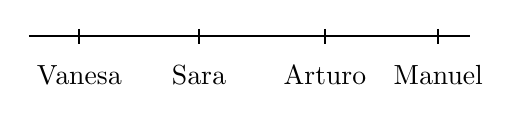
\begin{tikzpicture}[scale=0.8]
		\draw[thick] (0,0) -- (7,0);
		\foreach \x/\n in {0.8/Vanesa,2.7/Sara,4.7/Arturo,6.5/Manuel}
		\draw[thick] (\x,0.12) -- (\x,-0.12) node[below=4pt] {\n};
	\end{tikzpicture}
	
	De ahí:
	
	A. es verdadero
	
	B. es verdadero
	
	C. es falso
	
	D. es verdadero
	
	E. es verdadero
	
	\vspace{6mm}
	
	\item Se define los operadores:
	
	$a\%b=a+ab+b$
	
	$a\Delta b=a^2+ab-b^2$
	
	Calcule: $(2\%4)\%(3\Delta2)$
	
	\begin{enumerate}[label=\alph*)]
		\item 179
		\item 169
		\item 160
		\item 168
		\item 178
	\end{enumerate}
	\textbf{Respuesta correcta:} a)
	
	\vspace{2mm}
	\textbf{Solucionario:}\\[1mm]
	
	\textit{i)} $2\%4=2+2(4)+4=14$
	
	\textit{ii)} $3\Delta2=3^2+3(2)-2^2=11$
	
	\textit{iii)} $14\%11=14+14(11)+11=14+154+11$
	
	\fbox{$=179$}
	
	\vspace{6mm}
	
	\item Calcule la suma
	
	$S=1+2+3+\ldots+120$
	
	\begin{enumerate}[label=\alph*)]
		\item 7360
		\item 6260
		\item 6360
		\item 5360
		\item 7260
	\end{enumerate}
	\textbf{Respuesta correcta:} e)
	
	\vspace{2mm}
	\textbf{Solucionario:}\\[1mm]
	
	$S=\sum_{i=1}^{n} i=\sum_{i=1}^{120} i=\dfrac{n(n+1)}{2}$
	
	$=\dfrac{120(121)}{2}=60(121)$
	
	\fbox{$=7260$}
	
	\vspace{6mm}
	
\end{enumerate}



\subsection*{Razonamiento Verbal}

\begin{enumerate}[resume]

	
	\item Según la RAE, la palabra alumno proviene del latín alumnus, que significa; persona …
	\begin{enumerate}[label=\alph*)]
		\item Nueva en algún sitio o principiante en cualquier actividad u oficio.
		\item Con atraso intelectual
		\item Que recibe enseñanza, de un profesor o de la escuela
		\item Que carece de instrucción o conocimiento
		\item Que pretende alcanzar un empleo, cargo o distinción
	\end{enumerate}
	\textbf{Respuesta correcta:} c)
	
	\vspace{2mm}
	\textbf{Solucionario:}\\[1mm]
	Alumno es la persona \textbf{que recibe enseñanza} de un profesor o institución educativa.
	
	\vspace{6mm}
	
	\item El congreso de la República acaba de aprobar el retorno a la bicameralidad, \rule{2cm}{0.4pt} que la población había rechazado en el referéndum del 2018; \rule{2cm}{0.4pt}, no se ha respetado la voluntad popular.
	\begin{enumerate}[label=\alph*)]
		\item A pesar - es decir
		\item No obstante - por lo tanto
		\item Mientras tanto - mejor dicho
		\item Es decir - no obstante
		\item Mientras - ya que
	\end{enumerate}
	\textbf{Respuesta correcta:} a)
	
	\vspace{2mm}
	\textbf{Solucionario:}\\[1mm]
	La secuencia marcada es \textbf{A pesar - es decir}, que enlaza concesión y explicación según el ejercicio.
	
	\vspace{6mm}
	
	\item El antónimo de DISPLICENCIA es:
	\begin{enumerate}[label=\alph*)]
		\item Licencia
		\item Acato
		\item Deferencia
		\item Jocosidad
		\item Probidad
	\end{enumerate}
	\textbf{Respuesta correcta:} c)
	
	\vspace{2mm}
	\textbf{Solucionario:}\\[1mm]
	“Displicencia” implica desdén o falta de consideración; su antónimo es \textbf{deferencia}.
	
	\vspace{6mm}
	
	\item Encuentre la oración donde se comete anfibología.
	\begin{enumerate}[label=\alph*)]
		\item Mañana tendrá lugar el reencuentro ¡Mejor!
		\item Encontraron una jauría de perros.
		\item Recomendé a Rosa a mi jefe
		\item Ella se lima las uñas con una lima.
		\item La dama, da el dado a David
	\end{enumerate}
	\textbf{Respuesta correcta:} c)
	
	\vspace{2mm}
	\textbf{Solucionario:}\\[1mm]
	“Recomendé a Rosa a mi jefe” es ambigua, por eso presenta \textbf{anfibología}.
	
	\vspace{6mm}
	
	\item PLAN DE REDACCIÓN\\
	El diccionario de sinónimos\\
	I. El diccionario de sinónimos presenta palabras en orden alfabético, con la particularidad de agruparlas según su semejanza significativa.\\
	II. Otras veces debemos buscar una palabra que se adecúe mejor a las circunstancias.\\
	III. Un diccionario general explica los significados y usos de las palabras de un idioma, alfabéticamente ordenadas.\\
	IV. Existen, por otro lado, diccionarios específicos como el de sinónimos.\\
	V. Un ejemplo de su uso lo tenemos cuando al escribir requerimos de un término que evite la repetición monótona de otro ya expresado anteriormente.
	\begin{enumerate}[label=\alph*)]
		\item V – IV – III – I – II.
		\item III – IV – V – IV – I.
		\item I – II – V – IV – III.
		\item I – III – IV – V – II.
		\item III – IV – I – V – II.
	\end{enumerate}
	\textbf{Respuesta correcta:} e)
	
	\vspace{2mm}
	\textbf{Solucionario:}\\[1mm]
	El orden lógico parte del diccionario general, pasa al específico y luego explica su uso: \textbf{III – IV – I – V – II}.
	
	\vspace{6mm}
	
	\item Lain Estralgo, ex director de la Real Academia, señalada: “el neologismo es ineludible, pero se deben tener en cuenta la necesidad, la adecuación y el buen linaje, o lo que es lo mismo, las raíces del griego, el latín y el buen castellano”, Feijoo sostenía: “para introducir una voz nueva, a falta absoluta de otra que signifique lo mismo, basta que la nueva tenga o más propiedad, o más hermosura, o más gracia”.\\
	Wenceslao Ortega.\\
	Tanto Lain Estralgo como Feijoo se pronuncian sobre:
	\begin{enumerate}[label=\alph*)]
		\item La importancia del neologismo en la estética del lenguaje.
		\item Las raíces griegas y latinas de todos los neologismos.
		\item La gran variedad de neologismos propios del castellano.
		\item Los factores que determinan la aceptación del neologismo.
		\item El neologismo y sus diferentes utilidades para los artistas.
	\end{enumerate}
	\textbf{Respuesta correcta:} d)
	
	\vspace{2mm}
	\textbf{Solucionario:}\\[1mm]
	Ambos autores tratan sobre los criterios o \textbf{factores de aceptación del neologismo}.
	
	\vspace{6mm}
	
\end{enumerate}

\subsection*{Inglés}

\begin{enumerate}[resume]

	
	\item Complete the conversation.\\
	A: \rule{6cm}{0.4pt}\\
	B: No, they’re not accountants. They’re matematics.
	\begin{enumerate}[label=\alph*)]
		\item Are they accountants?
		\item Are you accountants?
		\item Is he accountant?
		\item Are they matematics?
		\item Does he matematic?
	\end{enumerate}
	\textbf{Respuesta correcta:} a)
	
	\vspace{2mm}
	\textbf{Solucionario:}\\[1mm]
	The correct question is: \textbf{Are they accountants?} because the answer says: “No, they’re not accountants.”
	
	\vspace{6mm}
	
	\item The last year was:
	\begin{enumerate}[label=\alph*)]
		\item Two thousand twenty four
		\item Two thousand fifty three
		\item Two thousand twenty three
		\item Two thousand ninety nine
		\item Two thousand sixty one
	\end{enumerate}
	\textbf{Respuesta correcta:} c)
	
	\vspace{2mm}
	\textbf{Solucionario:}\\[1mm]
	The marked correct option is \textbf{Two thousand twenty three}.
	
	\vspace{6mm}
	
\end{enumerate}

\subsection*{Quechua y Aimara}

\begin{enumerate}[resume]

	
	\item ¿Hayk’a p’unchaykunataq huk watapiri kan?/¿Qawqha urunisa ma maraxa?
	\begin{enumerate}[label=\alph*)]
		\item Kimsa pachaq suqta chunka pichqayuq p’unchaykuna/ kimsa pataka suxta tunka phisqani urunaka.
		\item Kimsa pachaq suqta chunka tawayuq p’unchaykuna/kimsa pataka suxta tunka pusini urunaka
		\item Kimsa pachaq suqta chunka iskayniyuq p’unchaykuna/kimsa pataka suxta tunka kimsani urunaka.
		\item Kimsa pachaq suqta chunka iskayniyuq p’unchaykuna/kimsa pataka suxta tunka payani urunaka.
		\item Kimsa pachaq suqta chunka qanchisniyuq p’unchaykuna/kimsa pataka suxta tunka paqallquni urunaka.
	\end{enumerate}
	\textbf{Respuesta correcta:} a)
	
	\vspace{2mm}
	\textbf{Solucionario:}\\[1mm]
	La opción marcada como correcta es la alternativa \textbf{a)}.
	
	\vspace{6mm}
	
	\item ¿Imatataq wakakunari mikhunku?/¿Kunsa wakanakaxa manq’apxi?
	\begin{enumerate}[label=\alph*)]
		\item Allpata/Laq’a
		\item Q’achuta/Chuxlla
		\item Unuta/uma
		\item Kachita/Jayu
		\item Rumita/Qala
	\end{enumerate}
	\textbf{Respuesta correcta:} b)
	
	\vspace{2mm}
	\textbf{Solucionario:}\\[1mm]
	La vaca come pasto o hierba, por ello la respuesta marcada es \textbf{Q’achuta/Chuxlla}.
	
	\vspace{6mm}
	
\end{enumerate}





